\documentclass[final,5p,times,twocolumn]{elsarticle}
\usepackage[T1]{fontenc}
\renewcommand{\ttdefault}{lmtt}
\usepackage{microtype,graphicx,booktabs,amsmath,amssymb,amsthm,array,tabularx,longtable,multirow}
\usepackage{xcolor,tikz,pgfplots,enumitem,placeins,xurl,needspace,etoolbox,balance}
\geometry{reset,a4paper,left=23mm,right=18mm,top=20mm,bottom=21mm,columnsep=6mm,footskip=10mm}
\usetikzlibrary{arrows.meta,positioning,calc,fit,matrix,backgrounds,patterns}
\pgfplotsset{compat=1.18}
\usepgfplotslibrary{groupplots}
\usepackage[hypertexnames=false,bookmarksnumbered=true,bookmarksopen=false]{hyperref}
\urlstyle{same}
\definecolor{linkblue}{HTML}{204D8B}
\hypersetup{colorlinks=true,linkcolor=linkblue,citecolor=linkblue,urlcolor=linkblue,pdfauthor={Chengzhan Li},pdftitle={Phase-Scoped Query Layouts for Reference-Preserving Speculative Decoding},pdfsubject={Complete article and supplement; final scope/state revision 2026-11-01}}
\definecolor{target}{HTML}{426B8B}
\definecolor{draft}{HTML}{936027}
\definecolor{qualified}{HTML}{3E725E}
\definecolor{aux}{HTML}{6B7075}
\definecolor{light}{HTML}{EDF1F3}
\newcommand{\QB}{\mathrm{QB}}
\newcommand{\PQ}{\mathrm{PQ}}
\newcommand{\GS}{\mathrm{GS}}
\newcommand{\MQ}{\mathrm{MQ}}
\newcommand{\kw}[1]{\texttt{#1}}
\newcommand{\same}{\textcolor{qualified}{\ensuremath{=}}}
\newcommand{\diff}{\textcolor{draft}{\ensuremath{\ne}}}
\newcommand{\sref}[1]{Supplement~\ref{#1}}
\newtheorem{proposition}{Proposition}
\newcolumntype{Y}{>{\raggedright\arraybackslash}X}
\setlength{\emergencystretch}{2em}
\setlength{\tabcolsep}{4pt}
\renewcommand{\arraystretch}{1.14}
\renewcommand{\bibfont}{\small\setlength{\baselineskip}{10.3pt}\raggedright\interlinepenalty=10000}
\setlist{nosep,leftmargin=*}
\setlength{\textfloatsep}{13pt plus 3pt minus 2pt}
\setlength{\dbltextfloatsep}{14pt plus 3pt minus 2pt}
\setlength{\floatsep}{11pt plus 2pt minus 2pt}
\setlength{\dblfloatsep}{12pt plus 2pt minus 2pt}
\setlength{\intextsep}{11pt plus 2pt minus 2pt}
\renewcommand{\topfraction}{0.9}
\renewcommand{\dbltopfraction}{0.9}
\renewcommand{\textfraction}{0.07}
\renewcommand{\floatpagefraction}{0.7}
\renewcommand{\dblfloatpagefraction}{0.7}
\setcounter{topnumber}{3}
\setcounter{dbltopnumber}{3}
\clubpenalty=8000
\widowpenalty=8000
\displaywidowpenalty=8000
\raggedbottom
\makeatletter
\def\ps@pprintTitle{\let\@oddhead\@empty\let\@evenhead\@empty\def\@oddfoot{\hfil\thepage\hfil}\let\@evenfoot\@oddfoot}
\makeatother
\tikzset{box/.style={draw=aux,rounded corners=1pt,align=center,inner sep=5pt,font=\small},flow/.style={-{Latex[length=2mm]},line width=.55pt,draw=aux}}

% Stable build metadata; no shell escape or external programs are needed.
\pdfinfoomitdate=1
\pdftrailerid{}
\pdfsuppressptexinfo=15

% Robust balancing with full-width floats at article and supplement ends.
% The balance package also balances the bibliography before the appendix clearpage.

\begin{document}
\begin{frontmatter}
\title{Phase-Scoped Query Layouts for Reference-Preserving Speculative Decoding}
\author{Chengzhan Li}
\address{University of Electronic Science and Technology of China, Chengdu, China\\[2pt]
{\normalfont\ttfamily\href{mailto:chengzhan.li@std.uestc.edu.cn}{chengzhan.li@std.uestc.edu.cn}}}
\begin{abstract}Preserving a deployed quantized model's output can change the economic case for speculative decoding. We present phase-scoped query-to-batch (QB) attention, which expresses independent queries through paired query/mask views and shared K/V storage while retaining batched projections and feed-forward computation. Phase-aware dispatch and layout-sensitive graph reuse integrate the transformation with the native speculative transaction. A registered seven-arm study measures repair scope and drafting on two fixed twelve-input panels across three dates. On Qwen3, the draft-on/off speed ratio rises from 0.835 under global serialization to 1.188 under QB; SmolLM2 remains faster without drafting, with a QB ratio of 0.805. The corresponding QB/GS changes in draft value are 1.424 and 1.176, positive on every date mean. These are complete-request effects; SmolLM2's recorded logical work also changes with scope. Separate three-family experiments find 2.83--6.17\% lower speculative request latency than explicit per-query attention (PQ), with bitwise PQ/QB correspondence in 72 attention contexts. A matched Qwen3 study retains the layout benefit with fresh contexts. On Vulkan, an eight-input producer--consumer experiment finds two cases where changing the producer state switches PQ/QB from divergence to preservation of an unchanged serial reference. A separate Llama counterexample retains PQ/QB agreement while both depart from that reference. The results establish an implementable local repair and show why its deployment requires joint evaluation of repair scope, producer state and complete-request cost.
\end{abstract}
\begin{keyword}
speculative decoding \sep execution geometry \sep numerical consistency \sep runtime graph transformation \sep state composition
\end{keyword}
\end{frontmatter}
\section{Introduction}
Speculative decoding reduces sequential target invocations by verifying several draft tokens together~\cite{leviathan2023,chen2023}. Verification changes the target's execution geometry. In a quantized deployment, that change can alter finite-precision evaluation and the resulting greedy response. For applications tied to an existing regression baseline, the cost of preserving that baseline enters the draft decision.

Where the numerical constraint is imposed matters. Global serialization (GS) processes target rows individually through projections, attention and feed-forward layers. Per-query attention (PQ) confines the separation to attention and retains batching around it, but constructs an attention subgraph for each query. We study the effect of this repair scope on draft profitability and provide a lower-cost representation of local attention repair.

Phase-scoped query-to-batch attention (QB) views Q as $(d,1,h,q)$ instead of $(d,q,h,1)$ and transforms the mask in parallel. Existing attention operators process each query as a separate batch instance while K/V storage remains shared within one sequence. Head mapping and ordered recombination retain the native attention semantics. Role/phase guards and a layout-sensitive graph cache keep the selected organization consistent with the speculative transaction.

Query independence is established attention structure. Batch-invariant kernels constrain reductions~\cite{thinkingmachines}; CoRun controls prefill and decode shapes~\cite{corun}; LLM-42 verifies a fast path against fixed-shape execution~\cite{llm42}. QB integrates the query view with the runtime using existing non-flash operators. Its evidence concerns agreement with a specified deployed numerical stack and the complete cost of qualified implementations.

The principal cost result comes from a registered GS/PQ/QB by draft-on/off study on the already-exposed Qwen3 and SmolLM2 transfer panels, using seven-arm input blocks on three dates. Qwen3's draft value rises from 0.835 under GS to 1.122 under PQ and 1.188 under QB; local repair changes its draft decision on every date. SmolLM2 remains faster without drafting under every scope. Its positive scope interaction reduces the drafting penalty without reversing the decision. The request-level estimate includes changes in logical work (Section~\ref{sec:scopefinal}). The earlier three-family comparison and six-session E2 study also measure local implementation cost: QB reduces speculative request latency over PQ by 2.83--6.17\%, and 72 fixed attention contexts establish bitwise PQ/QB correspondence.

The state supplied to a local repair also determines its reference behavior. In a controlled Vulkan experiment, two of eight inputs retain the same serial-reference endpoint under both prefill producers, yet PQ/QB preserve that reference under one producer and depart from it under the other. Both local consumers agree throughout. This result ties eligibility to the complete producer boundary state within the validated clean receiver. A Llama input-transfer counterexample and its separate diagnostic provide a distinct case where PQ/QB agree but neither preserves the reference. Qualification must cover both producer and consumer.

The contributions are:
\begin{enumerate}[label=(\arabic*),itemsep=2pt]
\item A phase-scoped attention transformation with paired Q/mask views, shared-KV and head semantics, ordered output recovery and layout-sensitive graph reuse.
\item Matched evidence that repair scope changes draft profitability, including a preregistered three-date transfer study and separate measurements of QB's PQ-relative cost.
\item Producer--consumer and backend interventions that establish concrete reference-qualification requirements, supported by complete request and native replay records.
\end{enumerate}
A matched Qwen3 deployment study additionally finds practical QB benefits at $k=3$ with both resident and fresh contexts~\cite{rtxnativebridge}. Cost comparisons use qualified combinations under a declared workload and service window. Its source package supplies reported-data reconstruction; native source kits, fixtures and reference archives have separate, authenticated access instructions~\cite{studyrecords,rtxnativedelivery,b570nativedelivery}.

\section{Reference contract and execution model}
\label{sec:contract}
\subsection{Output qualification}
Let $\rho$ identify the reference model and tokenizer bytes, prompt construction, numerical runtime, ordinary execution recipe, sampler and stopping rule. For input $x$, its endpoint is
\begin{equation}
\mathcal O_\rho(x)=(\mathbf y,\mathbf e,n,y_{\mathrm{last}},s),
\label{eq:endpoint}
\end{equation}
where $\mathbf y$ is the full native token-ID array, $\mathbf e$ its end-of-generation (EOG) flags, $n$ its length and $s$ the stop reason. The principal campaigns stop at native EOG or 128 generated tokens. A candidate qualifies on a registered panel $X$ when every required pair has $\mathcal O_c(x)=\mathcal O_\rho(x)$, the reference is stable and all required records are present. Latency comparisons use these qualified, complete responses.

We distinguish exact-arithmetic equivalence, bitwise operator correspondence and endpoint agreement. The tests address different parts of the execution contract. Backend acceptance and actual operator placement are additional execution prerequisites. Qualification refers to the stated configuration, panel and output window.

\subsection{Workload qualification and use}
The study selects implementations for declared, replayable workloads under a fixed reference. Three domains have distinct roles. The \emph{backend-admitted domain} comprises configurations accepted by the source and operator guards. The \emph{validated domain} comprises the inputs and output windows that pass complete-reference comparison under those configurations. The \emph{use domain} is the workload for which an implementation is selected after qualification. Admission alone does not certify numerical correspondence; the later Llama counterexample lies within the admitted configuration (Section~\ref{sec:transfer}).

For a workload requiring the deployed reference, the decision rule retains $R$ for inputs outside the validated domain and compares qualified candidates within it. Extending that domain requires fresh reference checks. This is an offline selection rule: the evaluated implementation has phase and configuration guards, but no online detector or recovery guarantee for arbitrary new inputs.

\subsection{The stateful transaction}
A target context owns KV values, sequence positions, a pending sampled token or available logits, and relevant sampler state. The draft has separate state. It proposes up to $k$ tokens; the target evaluates the pending token and proposal positions; acceptance, correction and any bonus determine the committed prefix. Rejected positions are reconciled before the next cycle. A visible token may still be pending evaluation into KV and must be consumed exactly once.

QB changes attention representation within the ordinary speculative verification and reconciliation transaction. Microbatch capacity $U$, occupied query count $q$, caller width and output reservation remain distinct. We write UB$n$ for a configured capacity of $n$. A caller containing $k+1$ rows can execute as several physical micrographs, so caller counts alone do not describe parallel work.

\subsection{Local repair and state composition}
The design objective is to minimize complete request time over tested implementations, subject to endpoint qualification. Write a request fragment as $D_g(P_g(x))$, where $P_g$ forms the state consumed by $D_g$ under execution organization $g$. Correspondence of $D_{\QB}$ and the reference on one input state $s_\rho$ does not establish correspondence on the different state $P_g(x)$.

For full stateful composition, a relation between candidate and reference states must hold initially, preserve the committed output at each transaction, and hold again after reconciliation. The experiments test these sufficient-condition premises empirically. Section~\ref{sec:state} examines two simpler assumptions often used in local reasoning: that endpoint-equivalent states have interchangeable components, and that enlarging a sufficient replacement preserves its effect.

\section{Phase-scoped query-layout design}
\label{sec:method}
\subsection{Separating attention from target-wide batching}
Figure~\ref{fig:design} contrasts the three repair organizations. GS processes target rows one at a time throughout projection, attention and the feed-forward network. PQ retains batched surrounding work but explicitly constructs an attention subgraph for each query and concatenates the results. QB retains that local one-column organization through a view: queries become separate batch instances of the existing attention operators. It does not serialize the surrounding layers or construct a distinct attention subgraph per query.

\begin{figure*}[t]
\centering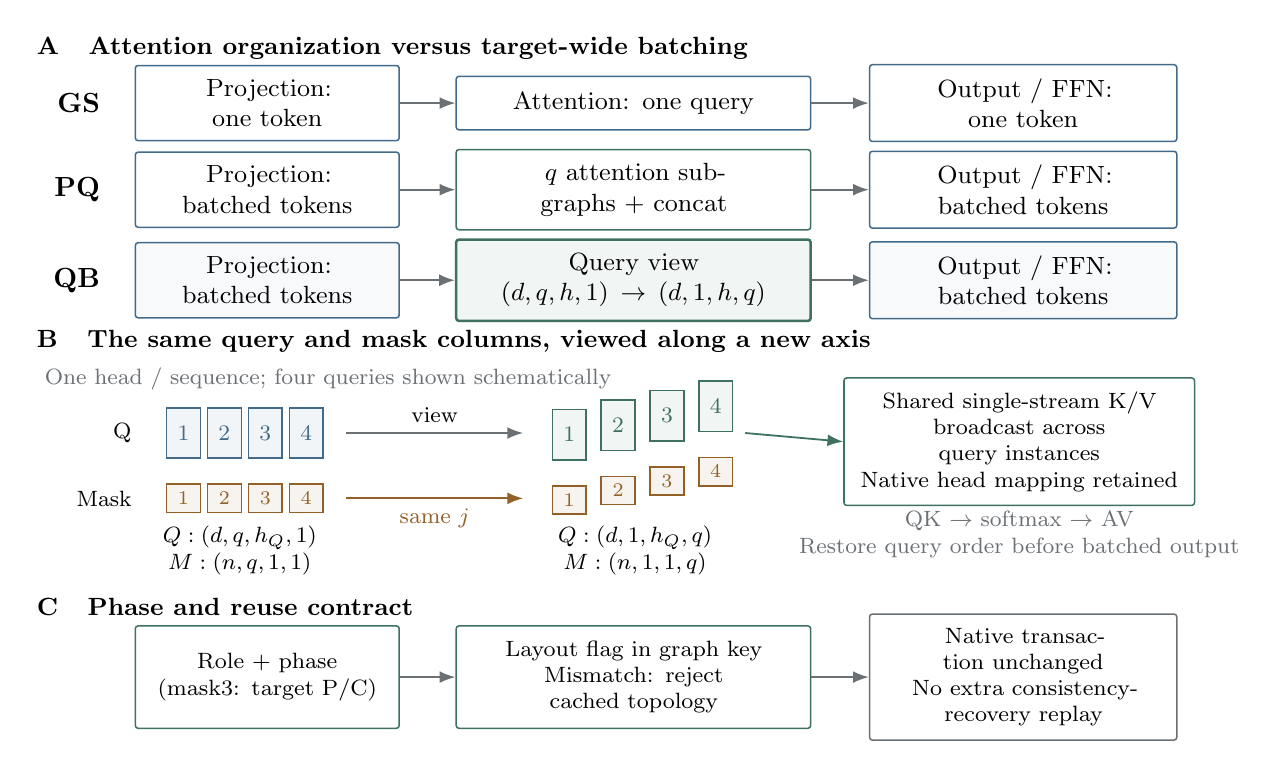
\begin{tikzpicture}[x=1cm,y=1cm,font=\small,
box/.append style={minimum height=.68cm,line width=.55pt},
flow/.append style={line width=.65pt}]
\node[anchor=west,font=\bfseries\small] at (0,4.05) {A\quad Attention organization versus target-wide batching};
\foreach \y/\lab in {3.35/GS,2.25/PQ,1.10/QB} {\node[anchor=east,font=\bfseries] at (1.05,\y) {\lab};}
\node[box,draw=target,text width=3cm] (g1) at (3.05,3.35) {Projection: one token};
\node[box,draw=target,text width=4.15cm] (g2) at (7.70,3.35) {Attention: one query};
\node[box,draw=target,text width=3.55cm] (g3) at (12.65,3.35) {Output / FFN: one token};
\node[box,draw=target,text width=3cm] (p1) at (3.05,2.25) {Projection:\\batched tokens};
\node[box,draw=qualified,text width=4.15cm] (p2) at (7.70,2.25) {$q$ attention subgraphs + concat};
\node[box,draw=target,text width=3.55cm] (p3) at (12.65,2.25) {Output / FFN:\\batched tokens};
\node[box,draw=target,fill=target!4,text width=3cm] (b1) at (3.05,1.10) {Projection:\\batched tokens};
\node[box,draw=qualified,fill=qualified!7,line width=.9pt,text width=4.15cm] (b2) at (7.70,1.10) {Query view\\$(d,q,h,1)\to(d,1,h,q)$};
\node[box,draw=target,fill=target!4,text width=3.55cm] (b3) at (12.65,1.10) {Output / FFN:\\batched tokens};
\foreach \a/\b in {g1/g2,g2/g3,p1/p2,p2/p3,b1/b2,b2/b3}\draw[flow] (\a)--(\b);
\node[anchor=west,font=\bfseries\small] at (0,.33) {B\quad The same query and mask columns, viewed along a new axis};
\node[anchor=west,font=\footnotesize,text=aux] at (.1,-.15) {One head / sequence; four queries shown schematically};
\foreach \j in {1,2,3,4} {
 \pgfmathsetmacro{\xx}{1.25+.52*\j}
 \draw[target,fill=target!7,line width=.55pt] (\xx,-1.16) rectangle ++(.43,.64);
 \node[font=\footnotesize,text=target] at (\xx+.215,-.84) {$\j$};
 \draw[draft,fill=draft!7,line width=.55pt] (\xx,-1.85) rectangle ++(.43,.36);
 \node[font=\scriptsize,text=draft] at (\xx+.215,-1.67) {$\j$};
 \pgfmathsetmacro{\bx}{6.05+.62*\j}\pgfmathsetmacro{\by}{-.98+.12*\j}
 \draw[qualified,fill=qualified!7,line width=.55pt] (\bx,\by-.32) rectangle ++(.43,.64);
 \node[font=\footnotesize,text=qualified] at (\bx+.215,\by) {$\j$};
 \draw[draft,fill=draft!7,line width=.55pt] (\bx,\by-1.01) rectangle ++(.43,.36);
 \node[font=\scriptsize,text=draft] at (\bx+.215,\by-.83) {$\j$};
}
\node[anchor=east,font=\footnotesize] at (1.45,-.84) {Q};
\node[anchor=east,font=\footnotesize] at (1.45,-1.67) {Mask};
\draw[flow] (4.05,-.84)--node[above,font=\footnotesize]{view} (6.3,-.84);
\draw[flow,draft] (4.05,-1.67)--node[below,font=\footnotesize]{same $j$} (6.3,-1.67);
\node[align=center,font=\footnotesize] at (2.70,-2.33) {$Q:(d,q,h_Q,1)$\\$M:(n,q,1,1)$};
\node[align=center,font=\footnotesize] at (7.72,-2.33) {$Q:(d,1,h_Q,q)$\\$M:(n,1,1,q)$};
\node[box,draw=qualified,text width=4.1cm,font=\footnotesize,minimum height=1.2cm] (sem) at (12.60,-.95) {Shared single-stream K/V\\broadcast across query instances\\Native head mapping retained};
\node[align=center,font=\footnotesize,text=aux] at (12.60,-2.13) {QK $\to$ softmax $\to$ AV\\Restore query order before batched output};
\draw[flow,qualified] (9.12,-.84)--(sem.west);
\node[anchor=west,font=\bfseries\small] at (0,-3.05) {C\quad Phase and reuse contract};
\node[box,draw=qualified,text width=3cm,font=\footnotesize,minimum height=1.3cm] (phase) at (3.05,-3.94) {Role + phase\\(mask3: target P/C)};
\node[box,draw=qualified,text width=4.15cm,font=\footnotesize,minimum height=1.3cm] (cache) at (7.7,-3.94) {Layout flag in graph key\\Mismatch: reject cached topology};
\node[box,draw=aux,text width=3.55cm,font=\footnotesize,minimum height=1.3cm] (native) at (12.65,-3.94) {Native transaction unchanged\\No extra consistency-recovery replay};
\draw[flow] (phase)--(cache);\draw[flow] (cache)--(native);
\end{tikzpicture}

\caption{Three same-reference implementation alternatives. Boxes show logical graph organization, not measured kernel occupancy. QB changes attention representation while keeping surrounding target computation batched. Numbered query and mask tiles depict logical indexing, not copied K/V or independent sequences. Phase selection is part of graph construction and reuse; the speculative transaction is unchanged.}
\label{fig:design}
\end{figure*}

We label the ordinary graph with multiple query positions MQ; this denotes execution geometry, not the multi-query attention (MQA) architecture with one shared K/V head. The intervention point follows the native Q/K/V permutations in the non-flash attention builder. Let $d$ be the query/key channel dimension, $q$ the number of occupied queries, $h_Q$ the query-head count, and $n$ the key extent. Using the runtime's axis order, the input query has shape $(d,q,h_Q, 1)$. QB creates a four-dimensional view with shape $(d, 1,h_Q,q)$ and preserves the original query-column stride as the new fourth-axis stride. The view retains the projected input values and token encoding.

\subsection{Address, mask and head semantics}
Write the original byte strides as $s_0,s_1,s_2,s_3$ and the base pointer as $b_Q$. For channel $i$, head $a$ and logical query $j$, the original address is
\begin{equation}
\operatorname{addr}_{\MQ}(i,j,a, 0)=b_Q+i s_0+j s_1+a s_2.
\end{equation}
The transformed view satisfies
\begin{equation}
\operatorname{addr}_{\QB}(i, 0,a,j)=b_Q+i s_0+a s_2+j s_1,
\label{eq:address}
\end{equation}
so it selects the same scalar. The singleton query-column stride is immaterial for access, but the implementation still supplies a valid native view descriptor. A strided source retains its actual strides.

The mask is transformed in parallel from $(n,q, 1,1)$ to $(n, 1,1,q)$. For original mask strides $m_0,m_1$, query $j$ still reads $b_M+t m_0+j m_1$ for key index $t$. The original mask values, including padded or disallowed positions, are retained. Changing the view must not replace a query-dependent causal mask by a single shared column. Logical token positions are unchanged: the new batch coordinate labels queries in one sequence, not independently positioned sequences.

Let $\kappa(a)$ denote the native grouped-query head mapping from query head $a$ to a K/V head. Under an integral grouped-query ratio, the same mapping is used by all three organizations. K and V retain their native values, strides and single-stream ownership and broadcast over the new query-batch coordinate. In mathematical notation, for the already implemented scaling $\alpha$ and admissible mask $m$,
\begin{align}
 z_{tja}&=\alpha\sum_i K_{it\kappa(a)}Q_{ija}+m_{tj},\\
 p_{tja}&=\frac{\exp(z_{tja})}{\sum_u\exp(z_{uja})},\\
 O_{vja}&=\sum_t V_{vt\kappa(a)}p_{tja}.
\label{eq:attn}
\end{align}
These equations describe logical indices; the actual runtime may store or permute V differently. QB must retain that implementation's mapping rather than reinterpret V by this notation alone.

\begin{proposition}[Mathematical view equivalence]
For a supported single-stream attention graph, suppose Equation~\eqref{eq:address} and the corresponding mask mapping hold, K/V broadcasting preserves $\kappa$, operator parameters are unchanged, and output recombination restores query order. In exact arithmetic, QB and the original attention graph compute the same logical $O$ in Equation~\eqref{eq:attn}.
\end{proposition}
\begin{proof}
For each fixed $(j,a)$, both representations select identical Q, K, V and mask values. The sums range over the same channel and key indices, and softmax is normalized over the same keys. The batch label in QB separates query instances but changes neither their operands nor their logical dependence. Recombination restores $(v,j,a)$ order. Thus every logical output value agrees in exact arithmetic. Finite-precision correspondence is established separately by the operator and complete-output experiments.
\end{proof}

After QK, softmax and AV, the native contiguous recombination restores the target's expected query/head order before its batched output projection. PQ realizes the same mathematical separation by slicing one query and its mask column per subgraph. The numerical and cost experiments test whether QB reproduces PQ's observed execution while avoiding its repeated subgraph structure.

\subsection{Admission conditions are part of the method}
The evaluated build admits one sequence/KV stream, non-flash attention, supported Qwen3 or dense Llama-family graph paths, compatible head dimensions, an integral GQA ratio, F32 query/mask values and F16 K/V. At most four queries are occupied in the current QB study. Attention bias, sinks and MLA value projections are excluded by the relevant source guards; other positional-bias schemes or unsupported strides require separate handling and validation. The mask may contain padded columns, but its first $q$ logical query columns and original key extent must be represented correctly.

These conditions preserve distinct meanings for sequence ownership, query indexing and head grouping. Additional streams need their own batch coordinate; biases and sinks need their own broadcasting rules. The source guards enforce the supported feature set, and each backend validates operator admission. Wider-geometry and fused-attention paths have separate numerical and execution contracts (\sref{supp:implementation}).

\subsection{Phase binding and graph-cache consistency}
The transformation is selected by a process-fixed four-bit mask: target prefill, target continuation, draft prefill and draft continuation have bits 1, 2, 4 and 8. Mask 3 enables the two target phases. A scoped guard derives the active flag from the current role and phase, places that flag in graph parameters, and restores its prior value on exit. New requests reset the phase to prefill. The guard executes before the observation-disabled fast path returns to native decoding; turning off a diagnostic callback must not disable the repair.

Graph reuse must preserve the selected layout. Two calls can share nominal capacity and tensor extents yet require different attention layouts. The reuse check includes the active-layout flag. A mismatch rejects reuse and requires an appropriate graph. The original campaigns fix the implementation choice (QB, PQ or GS) within each process. The later matched native bridge uses separate contexts for each layout within a process (Section~\ref{sec:matchedbridge}). Both keep the implementation fixed within a context; they do not validate dynamic PQ/QB switching under one cached graph. Table~\ref{alg:scope} summarizes the dispatch and reuse checks.

\begin{table}[t]
\caption{Phase-scoped dispatch and reuse obligations.}
\label{alg:scope}
\begin{tabularx}{\columnwidth}{@{}rX@{}}\toprule
1 & On request reset, establish target/draft ownership and set phase to prefill.\\
2 & Compute the role/phase bit and save the previous scope flag.\\
3 & Set the active flag before both observed and unobserved decode paths.\\
4 & If cached topology's layout flag differs, reject reuse.\\
5 & For an active supported attention graph, apply Q/mask views, native QK--softmax--AV and ordered recombination.\\
6 & Otherwise retain the declared untransformed graph or reject an unsupported active case.\\
7 & Complete native acceptance/state updates and restore the prior scope flag.\\\bottomrule
\end{tabularx}
\end{table}

Complete-output qualification covers the surrounding batched operators and the state they produce. The Vulkan projection interventions in Section~\ref{sec:state} locate this producer-side dependency.

\subsection{Selecting the active phases}
A prior four-switch experiment tested all 16 masks on four exposed HumanEval inputs at $k=3$, UB4 and cap128. Masks 3, 7, 11 and 15 passed both repetitions; mask3 was inclusion-minimal within that finite mask family. It was then fixed for the later model-family tests. The complete pattern and the separate mask3/mask15 cost comparison appear in \sref{supp:implementation}; that comparison did not pass its practical speed threshold.

\section{Experimental design}
\label{sec:experiments}
\subsection{Systems, panels and distinct evidence roles}
The implementation uses pinned llama.cpp/GGML sources~\cite{llamacpp,studyrecords}. CUDA experiments run on an RTX~5070~Ti Laptop GPU with Q8\_0 target/draft pairs: Qwen3-8B/0.6B~\cite{qwen3}, SmolLM2-1.7B-Instruct/135M-Instruct, and Llama-3.1-8B-Instruct/3.2-1B-Instruct. The models share a backend but include different head dimensions and attention-head mappings. Weight files and runtime libraries are byte-pinned, with exact versions recorded in the ancillary source manifest.

The ordinary CUDA reference uses physical UB1. Repaired execution uses target caller UB4, draft UB1, $k=3$, F16 KV, non-flash attention and context size 1024. The requested logical batch of 2048 is clamped to 1024; the frontend uses 24 host threads. One request is active at a time and prompt-cache reuse is disabled. The original Vulkan state studies instead use an Arc~B570 and Llama-3.1-8B-Instruct Q6\_K, with F16 KV, context 1024 and ten host threads. They are state and portability experiments, not a controlled comparison of GPU speed.

The core CUDA panels use sanitized MBPP and GSM8K inputs~\cite{mbpp,gsm8k}; HumanEval supplies engineering and Vulkan service probes~\cite{humaneval}. The transfer panel adds CodeContests programming tasks~\cite{rtxtransferrecords}. Outcomes are response preservation and runtime; Table~\ref{tab:campaigns} maps evidence to research questions.

\begin{table*}[t]\centering\small
\caption{Evidence organized by research question. Full panel identities, qualification counts and historical dispositions are retained in the supplement and ancillary inventory. Repeats are not independent tasks.}\label{tab:campaigns}
\begin{tabularx}{\textwidth}{@{}p{2.7cm}YY@{}}\toprule
Question & Principal evidence & Comparator and replication unit\\\midrule
Repair scope and draft value & Two exposed 12-input panels; 1,008 measurements over three dates & Seven arms; equal input, session and date log weights\\
Local representation cost & Three-family E2; six sessions and 864 local-arm measurements & PQ/QB, with target-only and speculative paths separate\\
Numerical correspondence & 72 captured contexts across families, layers, phases and widths & Same-input MQ/PQ/QB stage replay\\
Service deployment & Qwen3 $k=1,3$ by resident/fresh; six process sessions & Two identical PQ controls and QB under one timer\\
Reference transfer & 33/36 planned new-input cells reached; eight-input B570 state matrix & Strict $R$, own-producer C1 and local consumers\\
Composition and mapping & Whole-state/subset crosses and qualified backend/representation studies & Explicit receiver and complete transaction contracts\\\bottomrule
\end{tabularx}
\end{table*}

The 24-input output-confirmation panel was frozen after exclusion against accessible project execution history. The repair comparison and E2 reuse 12 exposed texts, six from each domain; the matched deployment study retains the Qwen3 panel. E1 selects one exposed prompt per family before capture. The new-input transfer panel is frozen separately after exclusion against project history. The three-date study reuses its Qwen3/SmolLM2 inputs after exposure; the B570 boundary panel is selected separately before forwards. Vulkan state interventions use two known divergent inputs, two stable controls and separately labelled synthetic prefixes. Each panel supports the claim listed in Table~\ref{tab:campaigns}.

\subsection{Matched alternatives and complete-request timing}
The seven repair-comparison arms are $R$, $M_{\QB}$, $C_{\QB}$, $M_{\PQ}$, $C_{\PQ}$, $M_{\GS}$ and $C_{\GS}$. $M$ is target-only; $C$ adds the same draft protocol. GS physically serializes active target rows without changing the registered draft or stopping rule. PQ and QB retain surrounding batching. The original campaign uses arm-specific workers and reverses their order in its second session. E2 retains $R$ and the four PQ/QB arms, using two serial-reference endpoints for each task/session.

The paid CUDA interval is a complete nonstreaming resident-process HTTP request, including encoding/submission, generation, response parsing and endpoint validation. Model loading, artifact writes, hashes and registered warmups are outside it. The counts channel adds no heavy tensor readback or observation synchronization. Diagnostic times are separate and are not subtracted from request measurements.

For task $i$, session $s$ and arms $a,b$, let $t_{i,s,a}$ be the registered request measurement, or the within-session median where repetitions are specified. We use equal task and session log weights:
\begin{equation}
S_{a/b}=\exp\!\left(\frac{1}{|\mathcal S|}\sum_s\frac{1}{|X|}\sum_i\log\frac{t_{i,s,a}}{t_{i,s,b}}\right).
\label{eq:ratio}
\end{equation}
Values above one favor the denominator. Full required pairs must qualify; missing and divergent records are retained without imputation. On a common paired panel, ratio products obey algebraic identities, but they do not decompose operator time.

E2 uses fresh processes, short PQ/QB blocks and counterbalanced order. Six sessions span 24.45 hours from first to last start, with at least one hour between a completion and the next start. The primary interval is the registered pointwise 95\% percentile bootstrap of six session-level log contrasts, using 10,000 resamples. Its sampling unit is the session and its target is the fixed 12-input panel on one host. The practical ratio threshold is 1.02: for PQ/QB, this corresponds to a QB latency reduction of $1-1/1.02\approx1.96\%$. The later service studies register a 2\% reduction relative to their PQ control mean. No request-level bootstrap, outlier trimming or significance-dependent stopping is used.

A secondary sensitivity analysis applies a two-sided Student $t_5$ interval to the same six session mean log contrasts and recomputes the estimate after omitting each session. The $t$ interval assumes independent, approximately normal session log means. It checks dependence on the interval method and individual sessions while retaining the registered bootstrap as primary.

The retrospective E2 draft-on/off analysis pairs the four local arms within each family/task/session. It applies the same equal log weights to $M_L/C_L$ and reports exploratory pointwise $t_5$ intervals across six session means. These contrasts were not preregistered, and their intervals provide no simultaneous-coverage guarantee. They use no additional requests and leave the registered PQ/QB estimands and intervals unchanged.

\subsection{Numerical and state controls}
E1 freezes actual Q/K/V/mask bytes, shapes, strides, head maps and parameters. Native MQ capture/replay correspondence, within-arm repeatability and capture-on/off endpoint equality precede PQ/QB comparison. Each of 72 fresh workers runs a counts warmup, a heavy capture and a counts observer control; MQ, PQ and QB are then replayed twice per context. A failed control withholds the corresponding numerical claim.

Vulkan interventions reconstruct a declared continuation boundary: complete sequence KV and positions, initial full FP32 logits consumed by the native greedy sampler, an empty generated prefix and correct pending-token ownership. Sixteen own-path shams precede whole-KV crosses. Subset tests retain recipient initial logits and verify actual imported bytes. Subsequent four-cell analyses compare full logits only at a shared consumed prefix.

The service and mapping studies specify their own reference and cost windows (Sections~\ref{sec:service} and \ref{sec:mappingcosts}); the matched deployment design changes $k$ and lifecycle within a common runtime (Section~\ref{sec:matchedbridge}). Campaign identities, amendments and execution dispositions are indexed in the supplement. The resident HTTP comparisons retain their stated $k=3$ policy, timer and task weights.


\subsection{Final scope-transfer and producer-boundary studies}
The three-date study prospectively registers $I=\log D_{\QB}-\log D_{\GS}$ for each of two families. Seven-arm blocks are contiguous within input; a frozen rotation balances arm positions to within one occurrence across the 72 blocks per family. The two session means receive equal weight within each date, and three date means receive equal weight overall. Complete qualification precedes timing. Shared binaries within each family remove the historical PQ executable-route difference from this cohort. The primary display shows all date means; the registered Bonferroni-adjusted $t_2$ intervals are secondary sensitivity summaries (\sref{supp:finaltransfer}).

The B570 boundary study uses an independent strict UB1/output1 reference for each input, natural producer C1 continuations and actual post-import readback. Historical controls include consumer-specific natural/resumed PQ and QB comparisons, rather than relying only on C1 restoration. Strict-reference equality and equality with each producer's own C1 are computed separately. The 152 requests are diagnostic and provide no formal performance estimate (Section~\ref{sec:producerfinal}).

\section{Repair scope and query-layout cost}
\label{sec:results}
\subsection{Three-date scope--draft transfer}
\label{sec:scopefinal}
For repair layout $L$, let $M_L$ denote target-only execution and $C_L$ the same layout with drafting. The draft value $D_L=T(M_L)/T(C_L)$ exceeds one when drafting reduces complete-request time. The scope interaction is $\Gamma=D_{\QB}/D_{\GS}$; it measures how the draft increment changes with repair scope. PQ provides the local-repair comparator needed to distinguish that change from QB's representation benefit.

The registered study uses all twelve Qwen3 and all twelve SmolLM2 inputs from the completed transfer panel~\cite{rtxscopetransfer}. These inputs were previously unused when selected for that earlier study and are exposed here. Within each family, the same executable, core, numerical libraries and model bytes supply $R$ and the six GS/PQ/QB by draft-on/off arms. Contexts are resident, kept separate by scope and cleared between requests; target UB4, draft UB1, $k=3$, F16 KV, non-flash attention and cap128/native EOG remain fixed. GS executes physical target width one while local repair retains surrounding multirow computation.

All 196 qualification requests pass before their family's timing. Twelve independently loaded family-session processes collect 1,008 measurements and 84 warmups over October 30, October 31 and November 1. Each input forms a contiguous seven-arm block with a frozen rotation; every date contains two sessions per family. The service timer charges reset/setup, both prefills, generation, transaction/state work, synchronization and result assembly. Model loading, context provisioning and post-request comparison/file writes are separate. This is a complete resident-service window, distinct from the original HTTP timer.

Figure~\ref{fig:scopefinal} shows every date mean. Qwen3 has $D_{\GS}=0.835$, $D_{\PQ}=1.122$ and $D_{\QB}=1.188$. Its draft decision crosses parity under both local repairs on all three dates. SmolLM2 has corresponding ratios 0.684, 0.805 and 0.805: target-only remains cheaper in every scope on every date. The QB/GS interactions are 1.424 and 1.176. A positive scope interaction does not require profitable drafting.

\begin{figure*}[t]\centering
% Generated from immutable session logs; ranges are observed date ranges.
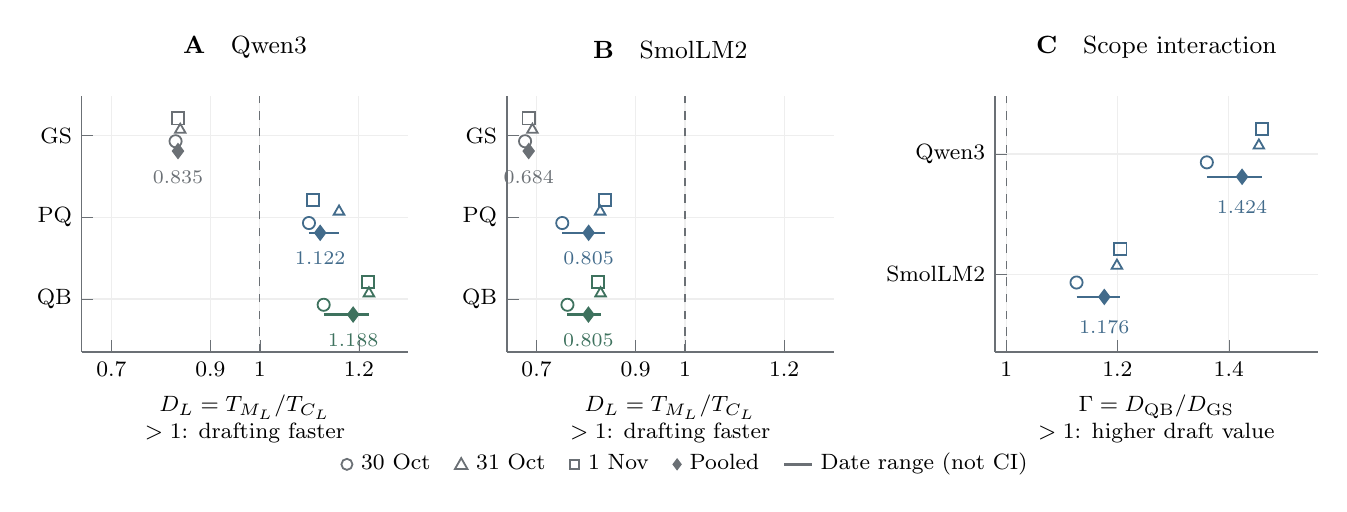
\begin{tikzpicture}
\begin{axis}[at={(0.6cm,0cm)},anchor=south west,scale only axis,
width=4.15cm,height=3.25cm,xmin=0.64,xmax=1.3,
ymin=.35,ymax=3.48,ytick={1,2,3},yticklabels={QB,PQ,GS},xtick={.7,.9,1,1.2},
axis lines*=left,axis line style={aux,line width=.5pt},tick style={aux},
tick label style={font=\footnotesize},grid=major,grid style={gray!13},
title={\textbf{A}\quad Qwen3},title style={font=\small,yshift=4pt},
xlabel={$D_L=T_{M_L}/T_{C_L}$\\$>1$: drafting faster},xlabel style={font=\footnotesize,align=center},clip=false]
\addplot[aux,dashed,forget plot] coordinates {(1,.35)(1,3.48)};
\addplot[aux,line width=.9pt,forget plot] coordinates {(0.829731004118,2.81)(0.839247877433,2.81)};
\addplot[only marks,mark=o,mark size=2.2pt,line width=.65pt,aux,forget plot] coordinates {(0.829731004118,2.93)};
\addplot[only marks,mark=triangle,mark size=2.2pt,line width=.65pt,aux,forget plot] coordinates {(0.839247877433,3.07)};
\addplot[only marks,mark=square,mark size=2.2pt,line width=.65pt,aux,forget plot] coordinates {(0.835003346314,3.21)};
\addplot[only marks,mark=diamond*,mark size=2.7pt,aux,forget plot] coordinates {(0.834651660975,2.81)};
\node[font=\scriptsize,text=aux,anchor=north] at (axis cs:0.834651660975,2.69){0.835};
\addplot[target,line width=.9pt,forget plot] coordinates {(1.099220287892,1.81)(1.159930527291,1.81)};
\addplot[only marks,mark=o,mark size=2.2pt,line width=.65pt,target,forget plot] coordinates {(1.099220287892,1.93)};
\addplot[only marks,mark=triangle,mark size=2.2pt,line width=.65pt,target,forget plot] coordinates {(1.159930527291,2.07)};
\addplot[only marks,mark=square,mark size=2.2pt,line width=.65pt,target,forget plot] coordinates {(1.107396324397,2.21)};
\addplot[only marks,mark=diamond*,mark size=2.7pt,target,forget plot] coordinates {(1.121863272924,1.81)};
\node[font=\scriptsize,text=target,anchor=north] at (axis cs:1.121863272924,1.69){1.122};
\addplot[qualified,line width=.9pt,forget plot] coordinates {(1.128912764045,0.81)(1.220335090837,0.81)};
\addplot[only marks,mark=o,mark size=2.2pt,line width=.65pt,qualified,forget plot] coordinates {(1.128912764045,0.93)};
\addplot[only marks,mark=triangle,mark size=2.2pt,line width=.65pt,qualified,forget plot] coordinates {(1.220335090837,1.07)};
\addplot[only marks,mark=square,mark size=2.2pt,line width=.65pt,qualified,forget plot] coordinates {(1.218401922887,1.21)};
\addplot[only marks,mark=diamond*,mark size=2.7pt,qualified,forget plot] coordinates {(1.188438428122,0.81)};
\node[font=\scriptsize,text=qualified,anchor=north] at (axis cs:1.188438428122,0.69){1.188};
\end{axis}
\begin{axis}[at={(6.0cm,0cm)},anchor=south west,scale only axis,
width=4.15cm,height=3.25cm,xmin=0.64,xmax=1.3,
ymin=.35,ymax=3.48,ytick={1,2,3},yticklabels={QB,PQ,GS},xtick={.7,.9,1,1.2},
axis lines*=left,axis line style={aux,line width=.5pt},tick style={aux},
tick label style={font=\footnotesize},grid=major,grid style={gray!13},
title={\textbf{B}\quad SmolLM2},title style={font=\small,yshift=4pt},
xlabel={$D_L=T_{M_L}/T_{C_L}$\\$>1$: drafting faster},xlabel style={font=\footnotesize,align=center},clip=false]
\addplot[aux,dashed,forget plot] coordinates {(1,.35)(1,3.48)};
\addplot[aux,line width=.9pt,forget plot] coordinates {(0.676863315065,2.81)(0.691715651785,2.81)};
\addplot[only marks,mark=o,mark size=2.2pt,line width=.65pt,aux,forget plot] coordinates {(0.676863315065,2.93)};
\addplot[only marks,mark=triangle,mark size=2.2pt,line width=.65pt,aux,forget plot] coordinates {(0.691715651785,3.07)};
\addplot[only marks,mark=square,mark size=2.2pt,line width=.65pt,aux,forget plot] coordinates {(0.684117166690,3.21)};
\addplot[only marks,mark=diamond*,mark size=2.7pt,aux,forget plot] coordinates {(0.684205177029,2.81)};
\node[font=\scriptsize,text=aux,anchor=north] at (axis cs:0.684205177029,2.69){0.684};
\addplot[target,line width=.9pt,forget plot] coordinates {(0.751980461104,1.81)(0.838157410742,1.81)};
\addplot[only marks,mark=o,mark size=2.2pt,line width=.65pt,target,forget plot] coordinates {(0.751980461104,1.93)};
\addplot[only marks,mark=triangle,mark size=2.2pt,line width=.65pt,target,forget plot] coordinates {(0.828542225334,2.07)};
\addplot[only marks,mark=square,mark size=2.2pt,line width=.65pt,target,forget plot] coordinates {(0.838157410742,2.21)};
\addplot[only marks,mark=diamond*,mark size=2.7pt,target,forget plot] coordinates {(0.805283741164,1.81)};
\node[font=\scriptsize,text=target,anchor=north] at (axis cs:0.805283741164,1.69){0.805};
\addplot[qualified,line width=.9pt,forget plot] coordinates {(0.762480613719,0.81)(0.829418625217,0.81)};
\addplot[only marks,mark=o,mark size=2.2pt,line width=.65pt,qualified,forget plot] coordinates {(0.762480613719,0.93)};
\addplot[only marks,mark=triangle,mark size=2.2pt,line width=.65pt,qualified,forget plot] coordinates {(0.829418625217,1.07)};
\addplot[only marks,mark=square,mark size=2.2pt,line width=.65pt,qualified,forget plot] coordinates {(0.824490025340,1.21)};
\addplot[only marks,mark=diamond*,mark size=2.7pt,qualified,forget plot] coordinates {(0.804876656398,0.81)};
\node[font=\scriptsize,text=qualified,anchor=north] at (axis cs:0.804876656398,0.69){0.805};
\end{axis}
\begin{axis}[at={(12.2cm,0cm)},anchor=south west,scale only axis,
width=4.1cm,height=3.25cm,xmin=0.98,xmax=1.56,
ymin=.35,ymax=2.48,ytick={1,2},yticklabels={SmolLM2,Qwen3},xtick={1,1.2,1.4},
axis lines*=left,axis line style={aux,line width=.5pt},tick style={aux},
tick label style={font=\footnotesize},grid=major,grid style={gray!13},
title={\textbf{C}\quad Scope interaction},title style={font=\small,yshift=4pt},
xlabel={$\Gamma=D_{\QB}/D_{\GS}$\\$>1$: higher draft value},xlabel style={font=\footnotesize,align=center},clip=false]
\addplot[aux,dashed,forget plot] coordinates {(1,.35)(1,2.48)};
\addplot[target,line width=.9pt,forget plot] coordinates {(1.360576811570,1.81)(1.459158131838,1.81)};
\addplot[only marks,mark=o,mark size=2.2pt,line width=.65pt,target,forget plot] coordinates {(1.360576811570,1.93)};
\addplot[only marks,mark=triangle,mark size=2.2pt,line width=.65pt,target,forget plot] coordinates {(1.454081831663,2.07)};
\addplot[only marks,mark=square,mark size=2.2pt,line width=.65pt,target,forget plot] coordinates {(1.459158131838,2.21)};
\addplot[only marks,mark=diamond*,mark size=2.7pt,target,forget plot] coordinates {(1.423873555506,1.81)};
\node[font=\scriptsize,text=target,anchor=north] at (axis cs:1.423873555506,1.69){1.424};
\addplot[target,line width=.9pt,forget plot] coordinates {(1.126491267510,0.81)(1.205188329550,0.81)};
\addplot[only marks,mark=o,mark size=2.2pt,line width=.65pt,target,forget plot] coordinates {(1.126491267510,0.93)};
\addplot[only marks,mark=triangle,mark size=2.2pt,line width=.65pt,target,forget plot] coordinates {(1.199074537459,1.07)};
\addplot[only marks,mark=square,mark size=2.2pt,line width=.65pt,target,forget plot] coordinates {(1.205188329550,1.21)};
\addplot[only marks,mark=diamond*,mark size=2.7pt,target,forget plot] coordinates {(1.176367387182,0.81)};
\node[font=\scriptsize,text=target,anchor=north] at (axis cs:1.176367387182,0.69){1.176};
\end{axis}
\node[anchor=north,font=\footnotesize] at (8.25,-1.15) {\tikz[baseline=-.5ex]\draw[aux,line width=.65pt] (0,0) circle (2pt);\ 30 Oct\quad \tikz[baseline=-.5ex]\draw[aux,line width=.65pt] (0,.08)--(.08,-.06)--(-.08,-.06)--cycle;\ 31 Oct\quad \tikz[baseline=-.5ex]\draw[aux,line width=.65pt] (-.06,-.06) rectangle (.06,.06);\ 1 Nov\quad \tikz[baseline=-.5ex]\fill[aux] (0,.08)--(.06,0)--(0,-.08)--(-.06,0)--cycle;\ Pooled\quad \tikz[baseline=-.5ex]\draw[aux,line width=.9pt] (0,0)--(.35,0);\ Date range (not CI)};
\end{tikzpicture}

\caption{Repair scope and draft value on the fixed two-family panel. A/B: same-layout target-only/speculative ratios, with a shared scale; values above one favor drafting. C: the complete-request interaction $\Gamma=D_{\QB}/D_{\GS}$, shown separately from profitability. Each open symbol is one of three actual date means; filled diamonds pool the dates with equal log weights. Segments span the observed date values, not confidence intervals; vertical offsets separate marks. Qwen3 crosses parity under local repair on all three dates. SmolLM2 has positive interaction but remains below draft parity.}
\label{fig:scopefinal}
\end{figure*}

Input log contrasts receive equal weight within session, sessions within date and dates overall. Every date and session mean has a positive interaction. Individual input/session reversals remain: 5/72 for Qwen3 and 27/72 for SmolLM2. The audit finds matched observed logical work across Qwen3's scopes. SmolLM2's work differs, so its estimate identifies a joint request-path effect rather than an execution-cost-only effect. No kernel-time decomposition follows from either ratio.

The three date interaction ranges are 1.361--1.459 for Qwen3 and 1.126--1.205 for SmolLM2. They provide evidence of direction stability over these dates on one host. The registered $t_2$ summaries are retained as weak, assumption-dependent sensitivity checks in \sref{supp:finaltransfer}, alongside all session points, secondary ratios and the execution amendment. The request count is not an independent date sample size.

\subsection{Original three-family comparison}
\label{sec:economics}
The original seven-arm study qualifies 96/96 endpoints per arm and family on a separate twelve-input panel. Its complete contrasts and Figure~\ref{fig:cost} remain in \sref{supp:cost}. Speculative GS/QB ratios of 2.144, 1.463 and 2.176 contrast global with local repair; PQ/QB ratios of 1.044, 1.068 and 1.022 measure QB's smaller representation increment. The original HTTP timer and two-session estimates remain separate from the three-date resident-service study.

A retrospective audit of all 2,016 measured responses reconstructs 288 matched seven-arm groups. All 1,728 within-path pairings agree in recorded logical-work counters and all 1,728 non-reference endpoints match paired $R$. Physical batching differs as intended. The groups match records across 42 arm-specific workers, not adjacent randomized execution blocks; their work agreement does not remove temporal drift (\sref{supp:sevenarmwork}).

The common-panel draft contrasts obey
\begin{equation}
D_L=\frac{S_{M_L/M_{\QB}}}{S_{C_L/C_{\QB}}}\,D_{\QB},\qquad D_{\QB}=S_{M_{\QB}/C_{\QB}},
\label{eq:draft}
\end{equation}
and the scope interaction is
\begin{equation}
\Gamma_{\QB\leftarrow\GS}=\frac{D_{\QB}}{D_{\GS}}
=\frac{S_{C_{\GS}/C_{\QB}}}{S_{M_{\GS}/M_{\QB}}}.
\label{eq:repairinteraction}
\end{equation}
Both PQ and QB make drafting profitable for Qwen3 and Llama on this original panel; SmolLM2 remains faster without drafting. The corresponding retrospective scope interactions are 1.612, 1.071 and 1.542. They describe common-panel request costs, not operator-time shares.

Target-only QB also preserves the reference at lower cost: $R/M_{\QB}=1.334051,1.369890,1.426161$, with every task favoring QB. Target-only QB is useful when drafting adds cost. These requests include prefill; target-only continuation uses the common one-query path. The larger-$k$ counterexample and all task regressions remain in Supplements~\ref{supp:implementation} and \ref{supp:cost}.

\subsection{Local draft decisions across E2 sessions}
\label{sec:e2draft}
A retrospective analysis pairs the 864 local-arm E2 measurements into 216 task/session quartets. Qwen3 and Llama favor drafting, while SmolLM2 favors target-only execution under both PQ and QB, in each of six sessions. Under QB, the pooled draft values are 1.084, 0.597 and 1.105. These estimates use the original exposed panel and separately scheduled local-arm blocks. E2 has no GS arm and therefore does not independently repeat the scope interaction. Full exploratory $t_5$ intervals and all original weights remain in \sref{supp:e2draft}.

\subsection{QB's independent implementation benefit}
\label{sec:e2}
The registered E2 comparison isolates representation cost within local repair. It completes 1,620 requests in 324 fresh workers, including 324 warmups and 432 serial-reference measurements. There are no request failures, output mismatches, workload errors or heavy-observer flags. The six-session speculative ratios $C_{\PQ}/C_{\QB}$ are 1.031614, 1.065803 and 1.029114, corresponding to 3.06\%, 6.17\% and 2.83\% lower QB request latency. Figure~\ref{fig:e2} shows both paths and their session-level uncertainty.

Table~\ref{tab:e2absolute} gives absolute costs from the source-verified requests, using the same task/session log weights.
\begin{table}[t]\centering\small
\caption{Absolute E2 request costs (ms), with equal task and session weights in the geometric mean. Registered warmups are excluded; the paid interval includes submission, full-response parsing and endpoint validation.}\label{tab:e2absolute}
\begin{tabular*}{\columnwidth}{@{\extracolsep{\fill}}lrrrr@{}}
\toprule
Family & $M_{\mathrm{PQ}}$ & $M_{\mathrm{QB}}$ & $C_{\mathrm{PQ}}$ & $C_{\mathrm{QB}}$ \\
\midrule
Qwen3 & 2130.4 & 2087.5 & 1987.2 & 1926.3 \\
SmolLM2 & 713.1 & 693.8 & 1238.8 & 1162.3 \\
Llama & 2574.7 & 2535.1 & 2360.9 & 2294.2 \\
\bottomrule
\end{tabular*}

\end{table}

\begin{figure*}[t]\centering
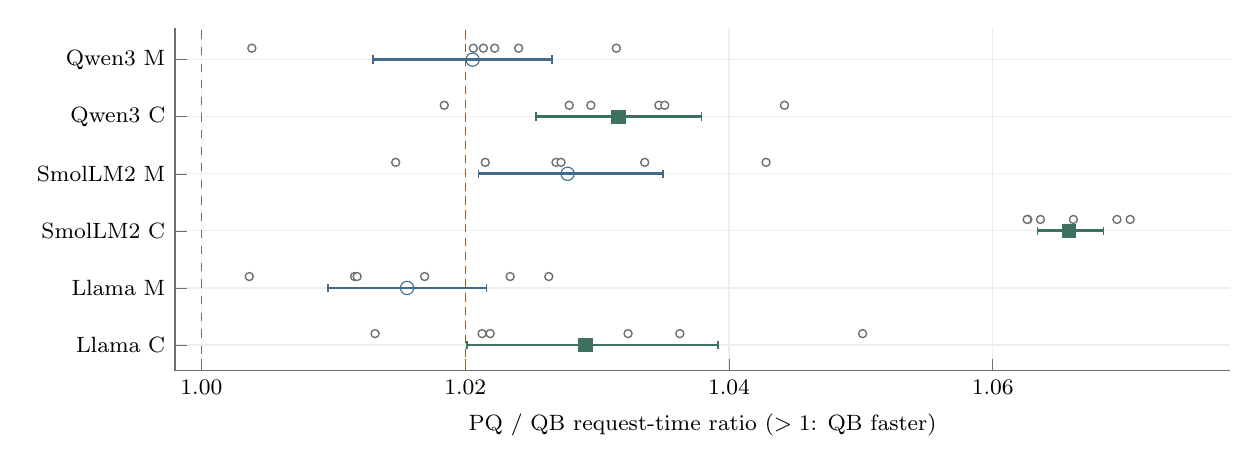
\begin{tikzpicture}[font=\footnotesize]
\begin{axis}[name=sess,scale only axis,width=13.4cm,height=4.35cm,
xmin=.998,xmax=1.078,xtick={1,1.02,1.04,1.06},xticklabels={1.00,1.02,1.04,1.06},
ymin=.55,ymax=6.55,ytick={6,5,4,3,2,1},yticklabels={Qwen3 M,Qwen3 C,SmolLM2 M,SmolLM2 C,Llama M,Llama C},
xlabel={PQ / QB request-time ratio ($>1$: QB faster)},xlabel style={font=\footnotesize},tick label style={font=\footnotesize},
axis lines*=left,axis line style={aux},tick style={aux},grid=major,grid style={gray!13}]
\draw[aux,dashed] (axis cs:1,.55)--(axis cs:1,6.55);
\draw[draft,densely dashed] (axis cs:1.02,.55)--(axis cs:1.02,6.55);
\addplot[only marks,mark=*,mark size=1.45pt,mark options={draw=aux,fill=white,line width=.5pt},color=aux] coordinates {(1.022241155,6.2) (1.003825879,6.2) (1.024056173,6.2) (1.031462696,6.2) (1.020617513,6.2) (1.021379783,6.2)};
\addplot[only marks,mark=*,mark size=1.45pt,mark options={draw=aux,fill=white,line width=.5pt},color=aux] coordinates {(1.018417206,5.2) (1.034686907,5.2) (1.029528424,5.2) (1.027889260,5.2) (1.044209114,5.2) (1.035132037,5.2)};
\addplot[only marks,mark=*,mark size=1.45pt,mark options={draw=aux,fill=white,line width=.5pt},color=aux] coordinates {(1.021523343,4.2) (1.042811401,4.2) (1.026887696,4.2) (1.027267920,4.2) (1.014728654,4.2) (1.033614105,4.2)};
\addplot[only marks,mark=*,mark size=1.45pt,mark options={draw=aux,fill=white,line width=.5pt},color=aux] coordinates {(1.062659839,3.2) (1.069420131,3.2) (1.066117550,3.2) (1.070418529,3.2) (1.063618892,3.2) (1.062610884,3.2)};
\addplot[only marks,mark=*,mark size=1.45pt,mark options={draw=aux,fill=white,line width=.5pt},color=aux] coordinates {(1.011619881,2.2) (1.003629727,2.2) (1.026339325,2.2) (1.016926078,2.2) (1.023407939,2.2) (1.011808397,2.2)};
\addplot[only marks,mark=*,mark size=1.45pt,mark options={draw=aux,fill=white,line width=.5pt},color=aux] coordinates {(1.013167868,1.2) (1.050133956,1.2) (1.021893776,1.2) (1.036275997,1.2) (1.032350688,1.2) (1.021280772,1.2)};
% Asymmetric percentile intervals and point estimates are generated from the frozen table.
\draw[target,line width=1pt] (axis cs:1.013022800003,6)--(axis cs:1.026553489035,6);
\draw[target,line width=.65pt] (axis cs:1.013022800003,5.925)--(axis cs:1.013022800003,6.075);
\draw[target,line width=.65pt] (axis cs:1.026553489035,5.925)--(axis cs:1.026553489035,6.075);
\addplot[only marks,mark=o,mark size=2.4pt,target] coordinates {(1.020563161899,6)};
\draw[qualified,line width=1pt] (axis cs:1.025392736138,5)--(axis cs:1.037925690306,5);
\draw[qualified,line width=.65pt] (axis cs:1.025392736138,4.925)--(axis cs:1.025392736138,5.075);
\draw[qualified,line width=.65pt] (axis cs:1.037925690306,4.925)--(axis cs:1.037925690306,5.075);
\addplot[only marks,mark=square*,mark size=2.4pt,qualified] coordinates {(1.031613690048,5)};
\draw[target,line width=1pt] (axis cs:1.021009792824,4)--(axis cs:1.035016679387,4);
\draw[target,line width=.65pt] (axis cs:1.021009792824,3.925)--(axis cs:1.021009792824,4.075);
\draw[target,line width=.65pt] (axis cs:1.035016679387,3.925)--(axis cs:1.035016679387,4.075);
\addplot[only marks,mark=o,mark size=2.4pt,target] coordinates {(1.027767425686,4)};
\draw[qualified,line width=1pt] (axis cs:1.063387048182,3)--(axis cs:1.068398798323,3);
\draw[qualified,line width=.65pt] (axis cs:1.063387048182,2.925)--(axis cs:1.063387048182,3.075);
\draw[qualified,line width=.65pt] (axis cs:1.068398798323,2.925)--(axis cs:1.068398798323,3.075);
\addplot[only marks,mark=square*,mark size=2.4pt,qualified] coordinates {(1.065803002589,3)};
\draw[target,line width=1pt] (axis cs:1.009627059351,2)--(axis cs:1.021621860041,2);
\draw[target,line width=.65pt] (axis cs:1.009627059351,1.925)--(axis cs:1.009627059351,2.075);
\draw[target,line width=.65pt] (axis cs:1.021621860041,1.925)--(axis cs:1.021621860041,2.075);
\addplot[only marks,mark=o,mark size=2.4pt,target] coordinates {(1.015593036909,2)};
\draw[qualified,line width=1pt] (axis cs:1.020125595877,1)--(axis cs:1.039148610748,1);
\draw[qualified,line width=.65pt] (axis cs:1.020125595877,0.925)--(axis cs:1.020125595877,1.075);
\draw[qualified,line width=.65pt] (axis cs:1.039148610748,0.925)--(axis cs:1.039148610748,1.075);
\addplot[only marks,mark=square*,mark size=2.4pt,qualified] coordinates {(1.029113522487,1)};
\end{axis}
\end{tikzpicture}

\caption{Independent-block E2 replication. Small marks are the six session estimates; large markers and horizontal bars are the equal-weight estimate and its registered 95\% six-session percentile interval. Dashed lines mark parity and the 1.02 practical threshold. $M$ is target-only and $C$ speculative. The fixed exposed panel and single host limit statistical scope.}
\label{fig:e2}
\end{figure*}

All 36 family/path/session contrasts favor QB; 9 of the 72 family/path/task aggregates regress. The primary pointwise speculative intervals are [1.025393,1.037926], [1.063387,1.068399] and [1.020126,1.039149], each above the predeclared 1.02 threshold under the registered percentile method. Target-only effects are smaller: Llama's estimate is 1.015593, below the threshold, while Qwen3's interval overlaps it.

The secondary $t_5$ intervals remain above 1.02 for speculative Qwen3 and SmolLM2. Llama's interval is [1.015387,1.043026], above parity but crossing 1.02; its six leave-one-session-out estimates range from 1.024960 to 1.032333. QB's advantage is stable in these checks. Whether the Llama effect exceeds the practical threshold depends on the interval method. \sref{supp:cuda} reports both analyses and all task regressions.

E2 establishes endpoint and recorded-counter correspondence across all 216 speculative PQ/QB task/session pairs: acceptance, rollback and logical-workload counters agree. This supports an implementation-cost comparison under matched recorded work. The original two-session estimates and their target-only direction reversals are reported in \sref{supp:cost}; E2's recorded-counter scope is detailed in \sref{supp:cuda}.

The recovered E2 records do not report actual CUDA Graph capture, replay or fallback counts. The request-cost estimate measures the implementation effect without isolating those mechanisms. The controlled QB/QH replay study in Section~\ref{sec:mappingcosts} has its own execution evidence and comparator.


\subsection{Same-input correspondence across layers and phases}
\label{sec:numeric}
The initial 24-context replay established PQ/QB correspondence at sampled layer-0 attention boundaries. E1 expands the test to three layer positions, prefill and continuation, and $q=1,2,3,4$ in each family. All 72 contexts pass observation, native-MQ own-path and repeatability checks. PQ and QB are bitwise equal at QK, softmax and AV in every context, with zero maximum error and ULP distance (Figure~\ref{fig:numeric}).

\begin{figure}[t]\centering
\resizebox{\columnwidth}{!}{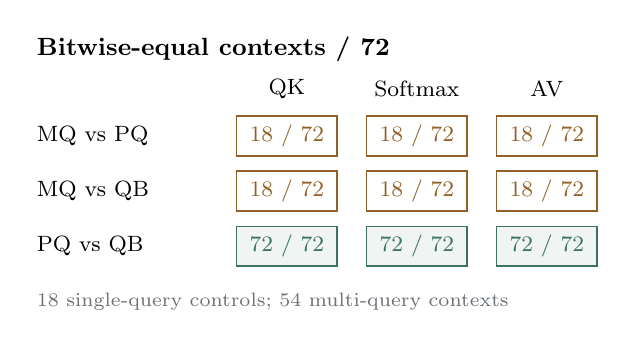
\begin{tikzpicture}[x=1cm,y=1cm,font=\footnotesize]
\node[anchor=west,font=\bfseries\small] at (0,2.65) {Bitwise-equal contexts / 72};
\foreach \x/\t in {3.30/QK,4.95/Softmax,6.60/AV}\node at (\x,2.15) {\t};
\foreach \y/\t in {1.55/MQ vs PQ,.85/MQ vs QB,.15/PQ vs QB}\node[anchor=west] at (0,\y) {\t};
\foreach \y in {1.55,.85}{\foreach \x in {3.30,4.95,6.60}{
 \draw[draft,line width=.65pt] (\x-.64,\y-.25) rectangle (\x+.64,\y+.25);
 \node[text=draft] at (\x,\y) {18 / 72};}}
\foreach \x in {3.30,4.95,6.60}{\draw[qualified,line width=.65pt,fill=qualified!8] (\x-.64,-.10) rectangle (\x+.64,.40);\node[text=qualified] at (\x,.15) {72 / 72};}
\node[anchor=west,text=aux,font=\scriptsize] at (0,-.55) {18 single-query controls; 54 multi-query contexts};
\end{tikzpicture}
}
\caption{Completed 72-context CUDA replay. The 18 agreements between MQ and either repair are exactly the $q=1$ common-path controls. The 54 multi-query cases first differ at QK. All PQ/QB stage outputs agree bitwise.}
\label{fig:numeric}
\end{figure}

The sampled target layers are $0/18/35$ for Qwen3, $0/12/23$ for SmolLM2 and $0/16/31$ for Llama. Qwen3 and Llama use head dimension 128 with 32 query heads and 8 KV heads; SmolLM2 uses dimension 64 with 32/32 heads. Thus the observed correspondence spans both ordinary and grouped-query attention and more than one head dimension.

MQ agrees with either repaired path only in the 18 single-query controls. Across the other 54 contexts, its first difference is at QK; maximum finite absolute differences are 0.078583 at QK, 0.000917 at softmax and 0.010433 at AV. These are operator differences on identical operands, not model-logit bounds.

All snapshots have tensor key extent 256, including masked padding. The maximum number of visible keys is 109, 130 and 127 by family; prefill captures include early query positions with only one to four visible keys. The experiment covers layers, phases and query widths at these short visible contexts, using one exposed prompt per family. Complete coordinates and operator comparisons appear in \sref{supp:cuda}.

\section{Complete-service deployment cost}
\label{sec:deployment}
\subsection{Matched deployment: k3 gains survive fresh contexts}
\label{sec:matchedbridge}
A new matched study separates the effects of speculative depth and context lifecycle within one runtime~\cite{rtxnativebridge}. It uses the original twelve exposed Qwen3 inputs, unchanged model/tokenizer bytes, context1024, target UB4, draft UB1 and cap128/native EOG. One executable supplies all four $k=1,3$ by resident/fresh cells and the PQ\_A/PQ\_B/QB arms. All 204 qualification requests preserve complete outputs and speculative state; corresponding PQ/QB decision vectors agree, and every output also matches the historical E2 reference.

Six independently loaded process sessions complete 864 measurements and 72 warmups. The order balances cells and arms within input/session blocks. Both models remain loaded. Resident requests clear their existing contexts; fresh requests create and destroy contexts inside the service timer. The shared timer includes prefill, generation, sampling, synchronization and result construction. Heavy capture and additional backend counters are disabled.

\begin{table*}[t]\centering\small
\caption{Matched Qwen3 deployment bridge. Ratios compare QB with the arithmetic mean of identical PQ controls; aggregation gives equal weight to inputs and process sessions. Intervals use the registered Bonferroni-adjusted bootstrap of six process sessions, with nominal 95\% family coverage across the four cells. The practical screen also requires reduction above the A/A threshold and improvement in every session.}
\label{tab:nativebridge}
\begin{tabular}{@{}rlll@{}}\toprule
$k$ & Lifecycle & QB/dual-PQ [adjusted interval] & Practical gain\\\midrule
1 & Resident & 0.986617 [0.965043, 1.006956] & Not established\\
3 & Resident & 0.937404 [0.922603, 0.949354] & Established\\
1 & Fresh & 0.973534 [0.955904, 0.996512] & Not established\\
3 & Fresh & 0.946409 [0.940517, 0.953312] & Established\\
\bottomrule\end{tabular}
\end{table*}


QB reduces service time by 6.26\% at resident $k=3$ and 5.36\% at fresh $k=3$ (Table~\ref{tab:nativebridge}). Both pass the registered practical screen; neither $k=1$ cell passes. The $k=3$ point reductions exceed their respective 4.125\% and 4.388\% input-aggregate A/A imbalances and favor QB in every session. The four primary intervals resample whole process sessions and use a Bonferroni adjustment; the twelve inputs remain a fixed panel.

The layout benefit survives fresh-context service at $k=3$. Secondary paired contrasts favor a stronger layout effect at $k=3$ in both lifecycles, while each individual lifecycle contrast includes parity. Changing $k$ changes the speculative transaction as well as query width. These comparisons identify a deployment-dependent layout effect, not a pure width intervention or a CUDA Graph mechanism. The new driver also does not reconstruct every difference between the older HTTP E2 and fresh-service contracts.


\subsection{Historical k1 service controls}
\label{sec:service}
The earlier RTX and B570 studies place the matched result in context. Both use Qwen3-8B/0.6B Q8\_0, $k=1$, F16 KV, non-flash attention and four exposed inputs. Their request formats, stopping windows, prefill policies and drivers differ. Each timer charges fresh-context creation, graph reservation, prefill, generation, synchronization and destruction, with model loading separate. Full contracts and all blocks appear in \sref{supp:service}~\cite{b570servicerecords,rtxservicerecords}.

The paired layout estimator uses two identical PQ controls:
\begin{equation}
\bar T_{is,\PQ}=\tfrac12(T_{is,\PQ_A}+T_{is,\PQ_B}),\qquad
r_{is}=T_{is,\QB}/\bar T_{is,\PQ}.
\label{eq:servicepair}
\end{equation}
Input/session ratios are combined with equal log weights. The finite-panel screen requires a reduction above both 2\% and the largest input-aggregate A/A imbalance, with improvement in every session. Both original panels fail this practical layout screen: QB/dual-PQ is 0.995144 on B570 and 0.989284 on RTX. The corresponding point reductions are 0.486\% and 1.072\%, against A/A imbalances of 0.754\% and 5.208\%; two of four RTX sessions favor PQ.

The speculative policy has a different outcome. On RTX, QB/R=0.582325 and dual-PQ/R=0.588633, so PQ already obtains most of the 41.8\% service-time reduction. On B570, QB/R=2.619763 under its separate two-model Vulkan contract. Its qualified R/PQ/QB requests match complete endpoints, 346 PQ/QB full-logit pairs and cycle traces, while costly draft work dominates the request. Changing the draft thread parameter produces DRAFT1/dual-baseline=1.003994~\cite{b570policyrecords}. The later CPU-draft prefill-submission study gives SUBMIT/dual-baseline=0.999161 and also fails its practical screen~\cite{b570prefillrecords}.

These controls distinguish the speculative policy's value from QB's incremental layout value. The common-runtime study above tests draft length and lifecycle directly; the original panels retain their separate references and timers. Their complete qualification, phase intervals, warmups and execution records remain in \sref{supp:service}.

\section{Reference transfer across inputs and backends}
\label{sec:state}
\subsection{Transfer to previously unexposed inputs}
\label{sec:transfer}
A separate study retains the three-family $k=3$ resident HTTP contract and preregisters twelve previously unexposed natural inputs per family~\cite{rtxtransferrecords}. The frozen panel covers formatted prompt-length strata 64--192, 256--448 and 640--832 within context1024. Short inputs are GSM8K mathematics; longer inputs are CodeContests code. Length and domain therefore vary together.

\begin{table*}[t]\centering\small
\caption{Transfer to previously unexposed inputs within context1024. Each family has a registered 12-input panel. Qwen3 and SmolLM2 complete all inputs; the Llama reference failure stops that family before cost measurement. The layout screen uses a 2\% floor, input-aggregate A/A and every-session direction; no population interval is assigned.}
\label{tab:heldouttransfer}
\begin{tabular}{@{}llll@{}}\toprule
Family & Reference qualification & QB/dual-PQ (screen) & QB/R\\\midrule
Qwen3 & 12/12 inputs pass & 0.967781 (not established) & 0.560577\\
SmolLM2 & 12/12 inputs pass & 0.930056 (pass) & 1.007007\\
Llama & PQ and QB both depart from R & Not run & Not run\\
\bottomrule\end{tabular}
\end{table*}


Qwen3 and SmolLM2 pass all twelve inputs. Four sessions per family supply 384 measurements and 384 warmups in total. SmolLM2's 6.99\% QB layout reduction passes the finite-panel practical screen, yet QB/R is 1.007007: the complete speculative request remains slightly slower than its serial reference. Qwen3's 3.22\% reduction is smaller than its 4.78\% A/A threshold. This distinguishes a PQ-relative layout saving from a gain over the serial reference.

Llama provides a reference-transfer counterexample. On CodeContests/valid/108, with 737 formatted prompt tokens, PQ and QB agree with each other in outputs, full decision vectors and causal trace, but both depart from deployed R at zero-based output index81. The remaining three Llama inputs and all Llama timing slots stay unexecuted. PQ/QB correspondence therefore does not establish reference preservation on a new input. The tested native-fast comparator also fails reference qualification in all three families; no qualified timing victory over that route is claimed. \sref{supp:followup} gives accounting and source access.


A separately registered 54-request diagnostic reproduces the known Llama failure and preserves two passing controls. For both P1 and P4\_NATIVE producer recipes, the known case's target-only C1 path matches historical $R$, while speculative PQ/QB agree with each other and depart from $R$. Observer-off/heavy comparisons preserve the same outcomes. These executions compare bundled natural recipes rather than importing a common state; the earliest internal operator divergence remains unresolved. Their clocks are excluded from performance results (\sref{supp:finaldiagnostic}).


\begin{figure*}[t]\centering
\resizebox{\textwidth}{!}{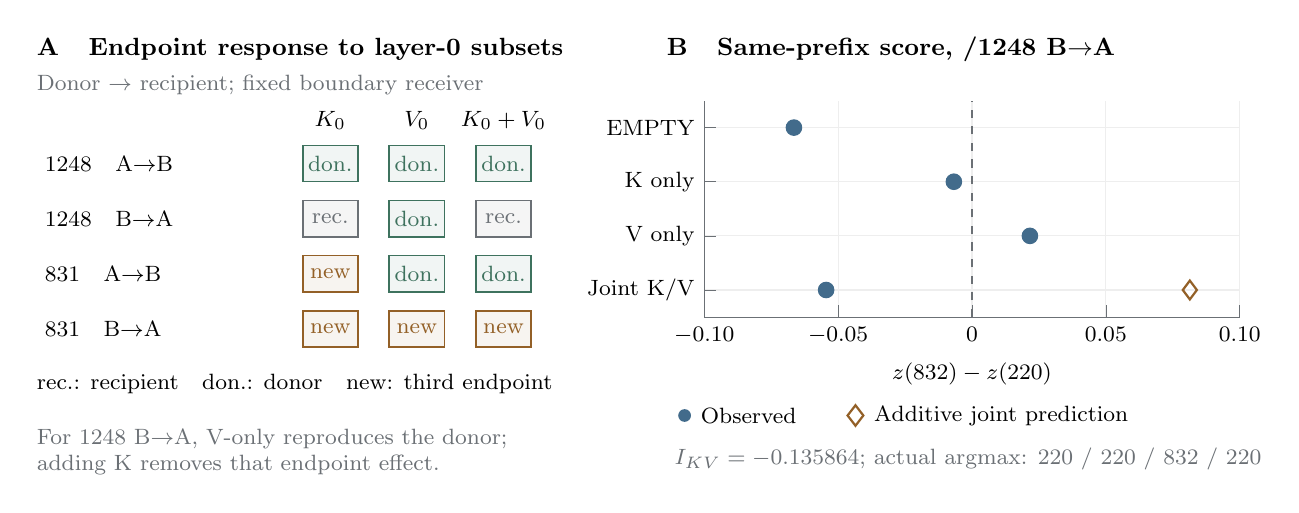
\begin{tikzpicture}[font=\footnotesize,x=1cm,y=1cm]
\node[anchor=west,font=\small\bfseries] at (0,4.4) {A\quad Endpoint response to layer-0 subsets};
\node[anchor=west,text=aux] at (0,3.95) {Donor $\to$ recipient; fixed boundary receiver};
\node at (3.85,3.5) {$K_0$};\node at (4.95,3.5) {$V_0$};\node at (6.05,3.5) {$K_0+V_0$};
\foreach \y/\lab in {2.95/{1248\quad A$\to$B},2.25/{1248\quad B$\to$A},1.55/{831\quad A$\to$B},.85/{831\quad B$\to$A}} {
 \node[anchor=west] at (.1,\y) {\lab};}
\foreach \x/\y/\v/\col in {3.85/2.95/B/qualified,4.95/2.95/B/qualified,6.05/2.95/B/qualified,3.85/2.25/D/aux,4.95/2.25/B/qualified,6.05/2.25/D/aux,3.85/1.55/C/draft,4.95/1.55/B/qualified,6.05/1.55/B/qualified,3.85/.85/C/draft,4.95/.85/C/draft,6.05/.85/C/draft}{
 \draw[\col,fill=\col!7,line width=.6pt] (\x-.35,\y-.23) rectangle ++(.7,.46);
 \if\v D\def\endpoint{rec.}\else\if\v B\def\endpoint{don.}\else\def\endpoint{new}\fi\fi
 \node[text=\col] at (\x,\y) {\endpoint};}
\node[anchor=west] at (0,.15) {rec.: recipient\quad don.: donor\quad new: third endpoint};
\node[anchor=north west,align=left,text=aux] at (0,-.3) {For 1248 B$\to$A, V-only reproduces the donor;\\adding K removes that endpoint effect.};
\node[anchor=west,font=\small\bfseries] at (8.0,4.4) {B\quad Same-prefix score, /1248 B$\to$A};
\begin{axis}[at={(8.6cm,1cm)},anchor=south west,scale only axis,width=6.8cm,height=2.75cm,
xmin=-.10,xmax=.10,xtick={-.10,-.05,0,.05,.10},xticklabels={$-0.10$,$-0.05$,0,0.05,0.10},
ymin=.5,ymax=4.5,ytick={4,3,2,1},yticklabels={EMPTY,K only,V only,Joint K/V},
axis lines*=left,axis line style={aux},tick style={aux},tick label style={font=\footnotesize},
xlabel={$z(832)-z(220)$},xlabel style={font=\footnotesize},grid=major,grid style={gray!13}]
\draw[aux,dashed] (axis cs:0,.5)--(axis cs:0,4.5);
\addplot[only marks,mark=*,mark size=2.8pt,target] coordinates {(-.06651496887207031,4)(-.006771087646484375,3)(.021633148193359375,2)(-.05448722839355469,1)};
\addplot[only marks,mark=diamond,mark size=3.4pt,draft,line width=.8pt] coordinates {(.08137702941894531,1)};
\end{axis}
\fill[target] (8.35,-.25) circle[radius=2.3pt];
\node[anchor=west,inner sep=0pt] at (8.55,-.25) {Observed};
\draw[draft,line width=.8pt] (10.42,-.25)--(10.52,-.12)--(10.62,-.25)--(10.52,-.38)--cycle;
\node[anchor=west,inner sep=0pt] at (10.75,-.25) {Additive joint prediction};
\node[anchor=west,text=aux] at (8.1,-.8) {$I_{KV}=-0.135864$; actual argmax: 220 / 220 / 832 / 220};
\end{tikzpicture}
}
\caption{State composition at two levels. A: layer-0 endpoint classes; rec. retains the recipient, don. reproduces a distinguishable donor and new is a third trajectory. Each cell has two agreeing process repeats. B: full-logit comparison for /1248, B$\to$A, at output 47 after a common consumed prefix. The hollow diamond is the additive prediction, not a fifth execution.}
\label{fig:composition}
\end{figure*}

\subsection{Qualify the producer state}
A local attention repair consumes state produced upstream. The B570 studies test whether prefill partitioning changes that state and the resulting single-query continuation. With target context UB512 and output capacity one, arm A submits the whole prompt; B splits it into 128 tokens and a remainder. Arm C uses UB128 with internal partitioning. All arms request final-position logits and then continue naturally.

For two exposed inputs of 161 and 133 prompt tokens, B reproduces C's complete endpoint, initial FP32 logits and sequence-KV bytes. A diverges at generated indices 47 and 81. Two longer controls have unequal A/B states but equal endpoints. A partition sweep yields several endpoint classes, including a third trajectory for the 133-token input split as $132+1$: smaller chunks are not monotonically closer to the reference (\sref{supp:b570}).

The differences begin before attention: first-layer K/V projections differ for the 161-token input, and Q/K/V differ for the 133-token input. Fixed-operand replay qualifies 32 of 40 calls and reproduces projection sensitivity. Eight scale/MUL calls are excluded because an in-place consumer overwrote their captured operands. The partition sweep is diagnostic because its driver body was authenticated after execution; the later replay has an authenticated admission record (\sref{supp:b570}).

A common UB512 receiver isolates the state link. It imports sequence KV and positions, samples the selected complete initial logits, and restores pending-token semantics. Sixteen own-path shams reproduce natural endpoints; 40 crosses then vary KV and logit sources. For the two affected tasks,
\begin{align}
Y(KV_A,L_A)=Y(KV_A,L_B)&=Y_A,\\
Y(KV_B,L_A)=Y(KV_B,L_B)&=Y_B.
\label{eq:cross}
\end{align}
All initial vectors choose token 1271, making the logit swap a first-decision negative control. The suffix follows the KV source; the stable controls retain their endpoint despite unequal KV. Local consumer qualification alone cannot certify the producer state. Transfer requires qualification of both.

\subsection{Endpoint agreement and state substitution}
\label{sec:composition}
The subset study tests ten selectors on four exposed inputs in both donor directions. After 32 EMPTY/ALL controls, 80 coordinates each run in two independent processes, with agreement at every coordinate. Of the 160 requests, 30 reproduce a distinguishable donor endpoint, 54 produce a third trajectory and 76 retain the recipient endpoint despite changed bytes (\sref{supp:composition}).

A layer-0 K-only or V-only replacement selects $1/64$ of total K/V value storage and can reproduce a donor endpoint. This sufficiency is nonmonotone. For /1248 B$\to$A, layer-0 V reproduces the donor, but adding K removes that effect. In the reverse direction, layer-0 V works while replacing V at every layer does not.

Endpoint equality also fails as a cache-substitution criterion. Natural A/B states for /1011 and /1249 have equal endpoints but unequal KV. On /1011, 16 of 20 subset/direction coordinates produce a third trajectory; all 20 retain the endpoint on /1249. These interventions refute arbitrary component interchangeability; they do not establish natural reachability of mixed states.

To distinguish additive changes crossing an argmax threshold from a nonadditive score response, we compare full FP32 logits at the first divergence after a common consumed prefix. For fixed tokens $(r,u)$, write $d_S=z_S(u)-z_S(r)$ and
\begin{equation}
I_{KV}=d_{KV}-d_K-d_V+d_\emptyset.
\label{eq:interaction}
\end{equation}
For /1248 B$\to$A at output 47, $(r,u)=(220,832)$. EMPTY/K/V/KV scores are $-0.066515$, $-0.006771$, $+0.021633$ and $-0.054487$. The additive prediction is $+0.081377$, opposite in sign to the observed joint score; $I_{KV}=-0.135864$. Full-vocabulary argmax tokens are 220/220/832/220. The result establishes a nonadditive response through subsequent computation, without localizing it to one kernel.

\sref{supp:composition} records the 44 complete contrasts among 112 planned repeat-level contrasts, canonical token coordinates and missing vectors.

\subsection{Qualify backend execution}
\label{sec:backend}
The original Vulkan pilot combines reference-like or bulk prefill with MQ, PQ or QB continuation. Reference monitoring fails the declared sampling schedule: 48 of 49 attempted requests complete, one is interrupted and 31 coordinates remain unstarted. Speculative QB also changes the /831 and /1011 outputs. The pilot fails qualification; \sref{supp:pilot} retains its full record.

Independent address and scalar oracles pass 432 synthetic fixtures over 72 geometries. Yet the original $q=2$ QB graph violates a necessary condition of the frozen Vulkan matrix-multiplication backend:
\begin{equation}
b_3(\mathrm{src}_0)=b_3(\mathrm{src}_1),
\label{eq:backend}
\end{equation}
where $b_3$ is the fourth tensor extent. QK pairs K at extent 1 with lifted Q at extent 2; AV pairs V at extent 1 with probabilities at extent 2. Both are rejected. MQ and each PQ slice satisfy this check with $(1,1)$.

The frozen backend rejects these lifted QK and AV descriptors because their fourth source extents differ. Actual placement and fallback transfers were not observed in the failed pilot; the later port addresses the source-level admission requirement directly.

\subsection{Preserving the AV path in a scoped GQA port}
A scoped port targets F16/F32, $d=128$, 32-query-head/8-KV-head layouts, physical key extents 256/512 and $q=2,4$. Its packed route matches PQ at QK and softmax but differs in 7,160 of 8,192 AV values at key512/$q=2$, with maximum absolute difference $1.22236\times10^{-9}$. That route fails the exact reference~\cite{b570gqarecords}.

The successful route reuses the existing noncontiguous AV shader with zero V batch stride, real probability/output strides and independent query workgroups. All six key256/512 by $q=1,2,4$ coordinates match byte-for-byte at QK, softmax, AV and final output; all 20 earlier PQ stage files remain unchanged. The port retains per-output evaluation while exposing parallel work across queries. Section~\ref{sec:service} qualifies this fixed-layout port in real requests; the earlier Llama Q6\_K pilot remains failed.


\subsection{Producer-conditioned reference eligibility}
\label{sec:producerfinal}
The successful port permits a controlled test of how producer state affects a local consumer. Eight natural mathematical inputs are selected by a frozen hash rule before new forwards: four GSM8K inputs of 64--192 tokens and four MATH-500 inputs of 256--352 tokens. A pre-forward source amendment and the original input strings are preserved in the evidence record~\cite{b570producer}.

The target producer uses PQ in both conditions. P1 submits one prompt ID per caller; P4T submits four, with a fixed three-token tail split into two plus one. Both request logits at the final prompt position only. The experiment saves the complete boundary state, including serialized sequence KV and initial FP32 logits, and restores it into a clean receiver. C1 continues target-only; PQ and QB consumers use the existing $k=1$ speculative transaction. Draft prefill is independently reconstructed under the same unchanged recipe. This isolates the defined target boundary-state intervention within the receiver contract.

All 32 historical observer and own-path controls pass before the 120 new-input requests. The full audit checks 96 actual restored boundaries and 88 observer/own-path comparisons. All eight P1+C1 endpoints match an independently executed strict $R$. Producer changes alter KV and initial logits on every input; PQ and QB agree in endpoints, cycles and captured full-vocabulary vectors in all sixteen input--producer pairs.

Figure~\ref{fig:producerfinal} retains the complete six-cell outcome for every input. On prealgebra/1865 and /1804, both natural C1 endpoints preserve the same $R$. Yet PQ/QB depart from $R$ after P1 and preserve it after P4T. Their first P1 departures are outputs 5 and 25, respectively (one-based). The supplied state changes local reference eligibility while the natural serial endpoint stays fixed. GSM8K/1184 is a distinct case: its natural C1 endpoint changes too, and local consumers depart from their own C1 under both producers. The remaining five inputs retain $R$ in all six cells.

\begin{figure*}[t]\centering
\resizebox{\textwidth}{!}{% Full 48-cell matrix in original input order; two fixed-R cases annotated.
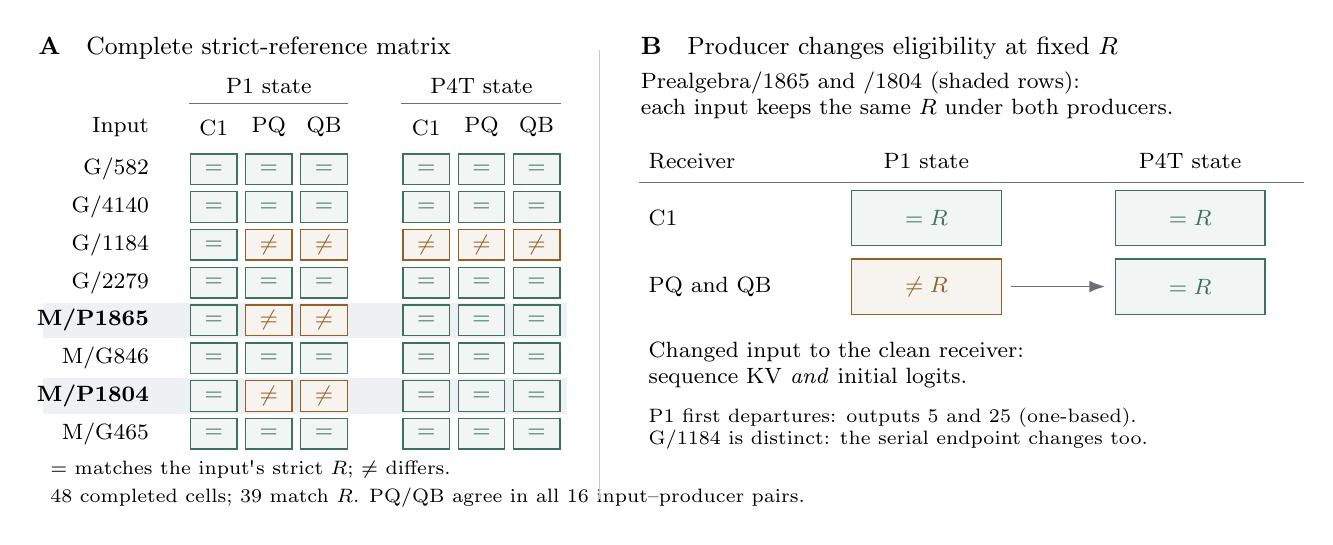
\begin{tikzpicture}[x=1cm,y=1cm,font=\footnotesize]
\node[anchor=west,font=\small] at (0,1.28) {\textbf{A}\quad Complete strict-reference matrix};
\node at (3.05,.80) {P1 state};
\node at (5.75,.80) {P4T state};
\draw[aux,line width=.45pt] (2.03,.57)--(4.06,.57);
\draw[aux,line width=.45pt] (4.73,.57)--(6.76,.57);
\node[anchor=east] at (1.65,.27) {Input};
\node at (2.35,.27){C1};
\node at (3.05,.27){PQ};
\node at (3.75,.27){QB};
\node at (5.05,.27){C1};
\node at (5.75,.27){PQ};
\node at (6.45,.27){QB};
\node[anchor=east] at (1.65,-0.260){G/582};
\node[draw=qualified,fill=qualified!7,line width=.5pt,minimum width=5.9mm,minimum height=3.9mm,inner sep=0pt,text=qualified] at (2.35,-0.260){$=$};
\node[draw=qualified,fill=qualified!7,line width=.5pt,minimum width=5.9mm,minimum height=3.9mm,inner sep=0pt,text=qualified] at (3.05,-0.260){$=$};
\node[draw=qualified,fill=qualified!7,line width=.5pt,minimum width=5.9mm,minimum height=3.9mm,inner sep=0pt,text=qualified] at (3.75,-0.260){$=$};
\node[draw=qualified,fill=qualified!7,line width=.5pt,minimum width=5.9mm,minimum height=3.9mm,inner sep=0pt,text=qualified] at (5.05,-0.260){$=$};
\node[draw=qualified,fill=qualified!7,line width=.5pt,minimum width=5.9mm,minimum height=3.9mm,inner sep=0pt,text=qualified] at (5.75,-0.260){$=$};
\node[draw=qualified,fill=qualified!7,line width=.5pt,minimum width=5.9mm,minimum height=3.9mm,inner sep=0pt,text=qualified] at (6.45,-0.260){$=$};
\node[anchor=east] at (1.65,-0.740){G/4140};
\node[draw=qualified,fill=qualified!7,line width=.5pt,minimum width=5.9mm,minimum height=3.9mm,inner sep=0pt,text=qualified] at (2.35,-0.740){$=$};
\node[draw=qualified,fill=qualified!7,line width=.5pt,minimum width=5.9mm,minimum height=3.9mm,inner sep=0pt,text=qualified] at (3.05,-0.740){$=$};
\node[draw=qualified,fill=qualified!7,line width=.5pt,minimum width=5.9mm,minimum height=3.9mm,inner sep=0pt,text=qualified] at (3.75,-0.740){$=$};
\node[draw=qualified,fill=qualified!7,line width=.5pt,minimum width=5.9mm,minimum height=3.9mm,inner sep=0pt,text=qualified] at (5.05,-0.740){$=$};
\node[draw=qualified,fill=qualified!7,line width=.5pt,minimum width=5.9mm,minimum height=3.9mm,inner sep=0pt,text=qualified] at (5.75,-0.740){$=$};
\node[draw=qualified,fill=qualified!7,line width=.5pt,minimum width=5.9mm,minimum height=3.9mm,inner sep=0pt,text=qualified] at (6.45,-0.740){$=$};
\node[anchor=east] at (1.65,-1.220){G/1184};
\node[draw=qualified,fill=qualified!7,line width=.5pt,minimum width=5.9mm,minimum height=3.9mm,inner sep=0pt,text=qualified] at (2.35,-1.220){$=$};
\node[draw=draft,fill=draft!7,line width=.5pt,minimum width=5.9mm,minimum height=3.9mm,inner sep=0pt,text=draft] at (3.05,-1.220){$\ne$};
\node[draw=draft,fill=draft!7,line width=.5pt,minimum width=5.9mm,minimum height=3.9mm,inner sep=0pt,text=draft] at (3.75,-1.220){$\ne$};
\node[draw=draft,fill=draft!7,line width=.5pt,minimum width=5.9mm,minimum height=3.9mm,inner sep=0pt,text=draft] at (5.05,-1.220){$\ne$};
\node[draw=draft,fill=draft!7,line width=.5pt,minimum width=5.9mm,minimum height=3.9mm,inner sep=0pt,text=draft] at (5.75,-1.220){$\ne$};
\node[draw=draft,fill=draft!7,line width=.5pt,minimum width=5.9mm,minimum height=3.9mm,inner sep=0pt,text=draft] at (6.45,-1.220){$\ne$};
\node[anchor=east] at (1.65,-1.700){G/2279};
\node[draw=qualified,fill=qualified!7,line width=.5pt,minimum width=5.9mm,minimum height=3.9mm,inner sep=0pt,text=qualified] at (2.35,-1.700){$=$};
\node[draw=qualified,fill=qualified!7,line width=.5pt,minimum width=5.9mm,minimum height=3.9mm,inner sep=0pt,text=qualified] at (3.05,-1.700){$=$};
\node[draw=qualified,fill=qualified!7,line width=.5pt,minimum width=5.9mm,minimum height=3.9mm,inner sep=0pt,text=qualified] at (3.75,-1.700){$=$};
\node[draw=qualified,fill=qualified!7,line width=.5pt,minimum width=5.9mm,minimum height=3.9mm,inner sep=0pt,text=qualified] at (5.05,-1.700){$=$};
\node[draw=qualified,fill=qualified!7,line width=.5pt,minimum width=5.9mm,minimum height=3.9mm,inner sep=0pt,text=qualified] at (5.75,-1.700){$=$};
\node[draw=qualified,fill=qualified!7,line width=.5pt,minimum width=5.9mm,minimum height=3.9mm,inner sep=0pt,text=qualified] at (6.45,-1.700){$=$};
\fill[light] (.18,-2.405) rectangle (6.84,-1.955);
\node[anchor=east,font=\footnotesize\bfseries] at (1.65,-2.180){M/P1865};
\node[draw=qualified,fill=qualified!7,line width=.5pt,minimum width=5.9mm,minimum height=3.9mm,inner sep=0pt,text=qualified] at (2.35,-2.180){$=$};
\node[draw=draft,fill=draft!7,line width=.5pt,minimum width=5.9mm,minimum height=3.9mm,inner sep=0pt,text=draft] at (3.05,-2.180){$\ne$};
\node[draw=draft,fill=draft!7,line width=.5pt,minimum width=5.9mm,minimum height=3.9mm,inner sep=0pt,text=draft] at (3.75,-2.180){$\ne$};
\node[draw=qualified,fill=qualified!7,line width=.5pt,minimum width=5.9mm,minimum height=3.9mm,inner sep=0pt,text=qualified] at (5.05,-2.180){$=$};
\node[draw=qualified,fill=qualified!7,line width=.5pt,minimum width=5.9mm,minimum height=3.9mm,inner sep=0pt,text=qualified] at (5.75,-2.180){$=$};
\node[draw=qualified,fill=qualified!7,line width=.5pt,minimum width=5.9mm,minimum height=3.9mm,inner sep=0pt,text=qualified] at (6.45,-2.180){$=$};
\node[anchor=east] at (1.65,-2.660){M/G846};
\node[draw=qualified,fill=qualified!7,line width=.5pt,minimum width=5.9mm,minimum height=3.9mm,inner sep=0pt,text=qualified] at (2.35,-2.660){$=$};
\node[draw=qualified,fill=qualified!7,line width=.5pt,minimum width=5.9mm,minimum height=3.9mm,inner sep=0pt,text=qualified] at (3.05,-2.660){$=$};
\node[draw=qualified,fill=qualified!7,line width=.5pt,minimum width=5.9mm,minimum height=3.9mm,inner sep=0pt,text=qualified] at (3.75,-2.660){$=$};
\node[draw=qualified,fill=qualified!7,line width=.5pt,minimum width=5.9mm,minimum height=3.9mm,inner sep=0pt,text=qualified] at (5.05,-2.660){$=$};
\node[draw=qualified,fill=qualified!7,line width=.5pt,minimum width=5.9mm,minimum height=3.9mm,inner sep=0pt,text=qualified] at (5.75,-2.660){$=$};
\node[draw=qualified,fill=qualified!7,line width=.5pt,minimum width=5.9mm,minimum height=3.9mm,inner sep=0pt,text=qualified] at (6.45,-2.660){$=$};
\fill[light] (.18,-3.365) rectangle (6.84,-2.915);
\node[anchor=east,font=\footnotesize\bfseries] at (1.65,-3.140){M/P1804};
\node[draw=qualified,fill=qualified!7,line width=.5pt,minimum width=5.9mm,minimum height=3.9mm,inner sep=0pt,text=qualified] at (2.35,-3.140){$=$};
\node[draw=draft,fill=draft!7,line width=.5pt,minimum width=5.9mm,minimum height=3.9mm,inner sep=0pt,text=draft] at (3.05,-3.140){$\ne$};
\node[draw=draft,fill=draft!7,line width=.5pt,minimum width=5.9mm,minimum height=3.9mm,inner sep=0pt,text=draft] at (3.75,-3.140){$\ne$};
\node[draw=qualified,fill=qualified!7,line width=.5pt,minimum width=5.9mm,minimum height=3.9mm,inner sep=0pt,text=qualified] at (5.05,-3.140){$=$};
\node[draw=qualified,fill=qualified!7,line width=.5pt,minimum width=5.9mm,minimum height=3.9mm,inner sep=0pt,text=qualified] at (5.75,-3.140){$=$};
\node[draw=qualified,fill=qualified!7,line width=.5pt,minimum width=5.9mm,minimum height=3.9mm,inner sep=0pt,text=qualified] at (6.45,-3.140){$=$};
\node[anchor=east] at (1.65,-3.620){M/G465};
\node[draw=qualified,fill=qualified!7,line width=.5pt,minimum width=5.9mm,minimum height=3.9mm,inner sep=0pt,text=qualified] at (2.35,-3.620){$=$};
\node[draw=qualified,fill=qualified!7,line width=.5pt,minimum width=5.9mm,minimum height=3.9mm,inner sep=0pt,text=qualified] at (3.05,-3.620){$=$};
\node[draw=qualified,fill=qualified!7,line width=.5pt,minimum width=5.9mm,minimum height=3.9mm,inner sep=0pt,text=qualified] at (3.75,-3.620){$=$};
\node[draw=qualified,fill=qualified!7,line width=.5pt,minimum width=5.9mm,minimum height=3.9mm,inner sep=0pt,text=qualified] at (5.05,-3.620){$=$};
\node[draw=qualified,fill=qualified!7,line width=.5pt,minimum width=5.9mm,minimum height=3.9mm,inner sep=0pt,text=qualified] at (5.75,-3.620){$=$};
\node[draw=qualified,fill=qualified!7,line width=.5pt,minimum width=5.9mm,minimum height=3.9mm,inner sep=0pt,text=qualified] at (6.45,-3.620){$=$};
\node[anchor=west,font=\scriptsize] at (.15,-4.08) {$=$ matches the input\textquotesingle s strict $R$; $\ne$ differs.};
\node[anchor=west,font=\scriptsize] at (.15,-4.43) {48 completed cells; 39 match $R$. PQ/QB agree in all 16 input--producer pairs.};
\draw[aux!40,line width=.45pt] (7.25,1.25)--(7.25,-4.45);
\node[anchor=west,font=\small] at (7.65,1.28) {\textbf{B}\quad Producer changes eligibility at fixed $R$};
\node[anchor=west,align=left] at (7.65,.68) {Prealgebra/1865 and /1804 (shaded rows):\\each input keeps the same $R$ under both producers.};
\node[anchor=west] at (7.75,-.15) {Receiver};
\node at (11.40,-.15) {P1 state};
\node at (14.75,-.15) {P4T state};
\draw[aux,line width=.45pt] (7.75,-.43)--(16.20,-.43);
\node[anchor=west] at (7.75,-.88) {C1};
\node[draw=qualified,fill=qualified!7,text=qualified,minimum width=19mm,minimum height=7mm] at (11.40,-.88) {$=R$};
\node[draw=qualified,fill=qualified!7,text=qualified,minimum width=19mm,minimum height=7mm] at (14.75,-.88) {$=R$};
\node[anchor=west] at (7.75,-1.75) {PQ and QB};
\node[draw=draft,fill=draft!7,text=draft,minimum width=19mm,minimum height=7mm] at (11.40,-1.75) {$\ne R$};
\node[draw=qualified,fill=qualified!7,text=qualified,minimum width=19mm,minimum height=7mm] at (14.75,-1.75) {$=R$};
\draw[flow] (12.47,-1.75)--(13.67,-1.75);
\node[anchor=west,align=left] at (7.75,-2.75) {Changed input to the clean receiver:\\sequence KV \emph{and} initial logits.};
\node[anchor=west,align=left,font=\scriptsize] at (7.75,-3.56) {P1 first departures: outputs 5 and 25 (one-based).\\G/1184 is distinct: the serial endpoint changes too.};
\end{tikzpicture}
}
\caption{Producer state and reference eligibility in the clean receiver. A: all 48 scientific cells in the original input order; symbols compare each endpoint with its input's fixed strict $R$. G is GSM8K; M/P and M/G are MATH-500 prealgebra and geometry. Shading identifies the two prealgebra cases expanded in B. Their serial C1 endpoints retain the same $R$, while PQ/QB switch from divergence to preservation. The intervention includes KV and initial logits; the arrow compares producer conditions, not temporal recovery. All 48 cells satisfy the evidence contract, and 39 match $R$.}\label{fig:producerfinal}
\end{figure*}

The intervention changes the complete producer boundary state, including initial logits; it does not identify KV alone as the cause. The tested boundary is the validated boundary0 clean receiver. Natural integrated P4T speculative execution and a specific earliest failing operator were not tested. Detailed schedules, all endpoint comparisons and access records are in \sref{supp:finalproducer}.

\subsection{Representation and execution-mode boundaries}
\label{sec:mappingcosts}
A local representation must also satisfy the reference after backend path selection and repay its conversion costs. Query-to-head mapping (QH) places independent queries in a head-like dimension and restores native output order. Balanced operator studies compare it with two identical QB controls under fixed inputs and execution windows~\cite{mappingrecords,b570compactrecords}.

On the RTX core panel, QB\_A/QH=0.900826. A frozen selector predicts all twelve held-out synthetic mean orderings, but its charged lookup raises the offline selector/fixed-QB estimate to 1.010298. CUDA Graph ON/OFF intervention reduces QB completed-graph cost to 0.615--0.849 of OFF and narrows four QH-minus-QB gaps from 12.056--12.975 to 0.735--1.627\,$\mu$s. These measurements establish execution-mode sensitivity of QB versus QH; the PQ/QB request comparison has a different comparator and lacks corresponding capture/replay counts.

Reference admission can exclude an otherwise faster execution path. RTX physical key extents 1023/1024/1025 select 8/3/8 kernels. Padding the same logical length-1023 operands and mask to extent1024 reaches three kernels on the first call but fails all four reference qualifications. Padding to1025 qualifies, retains eight kernels and costs about 1.5\% more than native QB (Figure~\ref{fig:mappingboundary}).

\begin{figure*}[t]
\centering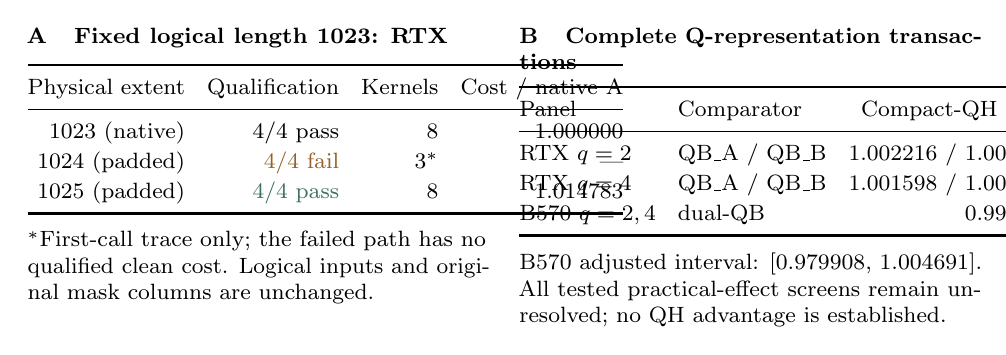
\begin{tikzpicture}[font=\footnotesize]
\node[anchor=north west,inner sep=0] at (0,0) {\begin{minipage}[t]{.48\textwidth}
\textbf{A\quad Fixed logical length 1023: RTX}\par\vspace{5pt}
\begin{tabular}{@{}rrrr@{}}\toprule
Physical extent & Qualification & Kernels & Cost / native A\\\midrule
1023 (native) & 4/4 pass & 8 & 1.000000\\
1024 (padded) & \textcolor{draft}{4/4 fail} & 3$^\ast$ & ---\\
1025 (padded) & \textcolor{qualified}{4/4 pass} & 8 & 1.014783\\\bottomrule
\end{tabular}\par\vspace{5pt}
$^\ast$First-call trace only; the failed path has no qualified clean cost. Logical inputs and original mask columns are unchanged.
\end{minipage}};
\node[anchor=north west,inner sep=0] at (.515\textwidth,0) {\begin{minipage}[t]{.48\textwidth}
\textbf{B\quad Complete Q-representation transactions}\par\vspace{5pt}
\begin{tabular}{@{}llr@{}}\toprule
Panel & Comparator & Compact-QH ratio\\\midrule
RTX $q=2$ & QB\_A / QB\_B & 1.002216 / 1.008295\\
RTX $q=4$ & QB\_A / QB\_B & 1.001598 / 1.004167\\
B570 $q=2,4$ & dual-QB & 0.992244\\\bottomrule
\end{tabular}\par\vspace{5pt}
B570 adjusted interval: [0.979908, 1.004691]. All tested practical-effect screens remain unresolved; no QH advantage is established.
\end{minipage}};
\end{tikzpicture}

\caption{Reference and transaction constraints on representation choice. A: padding the same logical length-1023 input to extent1024 selects a three-kernel path but fails all four reference checks. B: complete Q-representation transactions, with conversion and transfer charged. RTX and B570 use distinct geometries and execution modes; the B570 interval is descriptive and family-adjusted.}
\label{fig:mappingboundary}
\end{figure*}

Charging copy/transpose, upload, completed graph execution and ordinary-output readback removes the apparent compact-QH advantage. RTX compact-QH/QB\_A ratios are 1.002216 and 1.001598 at $q=2,4$, and neither passes the practical screen against both QB controls. The separate B570 transaction gives 0.992244 [0.979908,1.004691], also below the evidence required for a practical improvement. Fixed QB remains the selected baseline in these domains. Input-lifetime controls, continuous timer boundaries and all alternative mappings are detailed in \sref{supp:followupmapping}.

\section{Design implications}
\label{sec:decisionrule}
Repair scope, local representation and draft policy determine the cost of a reference-qualified combination. For a fixed experimental panel $X$, let $\mathcal A_\rho(X)$ contain the tested combinations that pass its complete-reference checks. A candidate with the lowest observed cost in that set is
\begin{equation}
a^\star=\arg\min_{a\in\mathcal A_\rho(X)} \widehat T_a(X),
\label{eq:policyselection}
\end{equation}
where $\widehat T_a$ uses the same service window and weights for every candidate. The objective compares the measured candidates. It supplies neither a classifier for new requests nor an online policy evaluated here. Qualification and deployment have the distinct roles defined in Section~\ref{sec:qualificationuse}.

\begin{table*}[t]\centering\small
\caption{Comparisons among tested execution combinations under one declared reference and service contract. The rows define evidence and estimands, not an online selection algorithm.}
\label{tab:deploymentrule}
\begin{tabularx}{\textwidth}{@{}>{\raggedright\arraybackslash}p{2.6cm}YY@{}}\toprule
Comparison & Evidence required & Interpretation\\\midrule
Reference eligibility & Supported layout, actual producer state and complete-output checks against $R$ & Identify the passing input/configuration pairs; source admission alone is insufficient.\\
Draft on or off & Target-only and speculative requests with the same repair, reference and timer & Measure the draft increment. Both local repairs make Qwen3 drafting profitable in the three-date panel; SmolLM2 favors target-only execution.\\
PQ or QB & Paired complete-request costs with the registered A/A and session controls & Measure the local representation increment. Matched Qwen3 $k=3$ passes under both lifecycles; $k=1$ remains unresolved.\\\bottomrule
\end{tabularx}
\end{table*}

\paragraph{Keep the three baselines distinct}
$R$ defines the behavior to preserve, same-layout $M_L$ measures the opportunity cost of enabling draft, and PQ isolates QB's representation increment. On the three-date SmolLM2 panel, $C_{\QB}$ costs 0.694295 of $R$, yet 1.242426 of $M_{\QB}$. A path can improve on the serial reference while remaining the more expensive draft decision. Table~\ref{tab:normalizedcosts} reports the common-panel ratios; its lowest point estimate is not a future-request policy.

\paragraph{Validate the producer--consumer relation}
Paired Q/mask views preserve query and head semantics; phase and layout flags preserve them during graph reuse. The Vulkan port retains the AV evaluation path while exposing independent query workgroups~\cite{b570gqarecords}. Its two fixed-$R$ cases show why a producer and a consumer passing separate tests does not qualify their combination. Validation must cover the state relation at their interface. Earlier component interventions further show that endpoint-equivalent states need not have interchangeable parts.

\paragraph{Charge the intended service transaction}
Matched Qwen3 $k=3$ requests retain practical QB benefits under resident and fresh contexts~\cite{rtxnativebridge}. The original $k=1$ panels, compact-QH transactions and B570 prefill-submission study retain distinct negative or unresolved outcomes. Their service windows include preparation and state costs omitted by local kernel or API-count comparisons.

These interfaces complement batch-invariant kernels~\cite{thinkingmachines}, reproducible accumulation~\cite{reproblas} and phase-aware tiled execution~\cite{spectra}. A hardware extension would preserve the declared per-query evaluation, including matrix-instruction behavior beyond dtype~\cite{ptx}, while sharing resources across queries. Establishing its benefit would require an equal-resource comparison on the request-critical path; the archived AV model supplies a same-policy parity control~\cite{studyrecords}.

\section{Related work and evidence scope}
\label{sec:related}
\subsection{Where numerical consistency is enforced}
Query-axis parallelism is established attention structure. FlashAttention uses tiled attention to reduce memory traffic~\cite{flashattention}; FlashAttention-2 distributes query rows across thread blocks and warps while sharing K/V~\cite{flashattention2}. These methods optimize fused evaluation and work partitioning. QB instead expresses independent queries through views of existing non-flash operators and integrates their one-query organization with phase selection, graph reuse and speculative state. Its qualification target is the output of a specified deployed numerical stack.

Table~\ref{tab:relatedmechanisms} compares the closest control points. Batch-invariant inference stabilizes reductions in normalization, matrix multiplication and attention~\cite{thinkingmachines}. CoRun combines isolated prefill, fixed-shape decode and selective kernel constraints~\cite{corun}. LLM-42 verifies fixed-shape windows and replaces decoded KV entries with verified entries even when token verification succeeds~\cite{llm42}. Vosti links canonical prefix-based KV state to relational kernel contracts and proves system-level determinism under its assumptions~\cite{vosti}. These guarantees apply to each system's execution contract. Compatibility with a separately chosen deployed quantized reference requires its own argument.

\begin{table*}[t]\centering\small
\caption{Numerical-consistency control points and guarantee scope. Performance comparisons here use GS and PQ in the same runtime; no common-contract speed ranking of these external systems is measured.}\label{tab:relatedmechanisms}
\begin{tabularx}{\textwidth}{@{}>{\raggedright\arraybackslash}p{2.3cm}>{\raggedright\arraybackslash}p{3.3cm}YY@{}}\toprule
Approach & Consistency target & Constraint and arithmetic & State and verification\\\midrule
Batch-invariant kernels~\cite{thinkingmachines}
& Each token's result is invariant to batching and slicing
& Stable reduction/tiling rules in kernels, including attention split size
& Consistent KV layout before attention; no added verify--rollback loop\\
CoRun~\cite{corun}
& Stable token sequence across co-runners, batch positions and arrival orders in a fixed stack
& Isolated prefill and fixed-shape CUDA-Graph decode; disable decode Split-KV and constrain collectives
& Request-local cache and RNG state; shape control supplies the execution contract\\
LLM-42~\cite{llm42}
& Tokens agree with a fixed-shape verification schedule
& Dynamic fast path plus fixed-shape replay; mostly existing kernels
& Verify--rollback; replace decoded KV with verified entries on acceptance as well as rollback\\
Vosti~\cite{vosti}
& Bitwise logits at corresponding positions across executions of a fixed configuration
& Runtime-independent kernel choices; verified relational contracts for selected kernels
& Canonical prefix-based KV invariant and an inductive engine proof under stated assumptions\\
Phase-scoped QB
& Complete output agrees with the specified ordinary reference on the qualified panel
& Q/mask views preserve local one-query attention; surrounding computation remains batched
& Finite producer--consumer qualification and native speculative reconciliation; no added online consistency verifier\\\bottomrule
\end{tabularx}
\end{table*}

QB's method is the integrated graph/runtime transformation. It reuses attention operators while changing query/mask representation, preserving head semantics and binding the layout to phases and graph identity. The Vulkan AV-preserving port shows that backend admission can still require an implementation change. Local numerical correspondence and stateful endpoint qualification test different parts of this contract.

Other approaches act at different boundaries. LayerCast separates storage and computation precision~\cite{layercast}; TBIK aligns reductions across tensor-parallel configurations~\cite{tbik}; MarginGate selects verification using decision margins~\cite{margingate}. The logical mapping proof, runtime guards, operator replay and endpoint tests in this work establish finite qualification against the specified reference.

\subsection{State and request cost}
Stage-Replay demonstrates suffix sensitivity to KV transplantation~\cite{stagereplay}, and cache-dependent divergence is reported in quantized serving~\cite{cachestate}. Our fixed-precision interventions add component-substitution counterexamples, common-prefix scores and a producer-conditioned eligibility test on the successfully ported Qwen3 consumer. Activation-patching studies establish the importance of intervention metrics and nonadditive component effects~\cite{patching,mediators}; our four-cell score contrast tests nonadditivity beyond an endpoint pattern caused only by thresholding.

Ragged-batch synchronization errors supply a separate source of speculative failures~\cite{forensics}. We check semantic indexing, finite-precision correspondence and backend admission separately. Work on verification cost and actual execution behavior~\cite{illusion,lossless} also motivates complete-request measurement. Our matched comparisons add the repair--draft interaction and isolate QB's incremental cost relative to PQ.

\subsection{Scope of the empirical results}
The CUDA request results cover one sequence, non-flash attention, $q\leq4$, Q8\_0 weights, F16 KV and context1024. E2 estimates variation across six sessions on one host for a fixed 12-input panel; E1 samples one prompt per family at physical key extent 256 and short visible contexts. The new-input study extends formatted prompts to 811 tokens and observed continuation visibility to 938 keys. Its short mathematical and longer programming inputs vary domain and length together~\cite{rtxtransferrecords}. The Llama counterexample in Section~\ref{sec:transfer} bounds reference transfer. All three families reject the tested native-fast comparator, so qualified cost comparisons remain against the declared serial and repaired paths.

The historical Vulkan state interventions concern four exposed inputs and finite greedy continuations. The final producer--consumer study adds eight mathematical inputs selected before forwards; the two source pools occupy different length bands. Its effect concerns complete boundary state under a clean receiver, with no KV-only or natural integrated P4T claim. The stopped Llama Q6\_K pilot remains unqualified. The Qwen3 Q8\_0 port has its own reference and runtime; native replay covers four complete requests, a real layer-0/key512/$q=2$ fixture and its first-query $q=1$ slice~\cite{b570nativereproduction}. The historical $k=1$ service and prefill-submission screens, including the latter's incomplete helper-process accounting, are retained in \sref{supp:service}.

The matched Qwen3 study estimates a joint draft-length/lifecycle contrast on twelve exposed inputs. Its six process sessions occur on one date; the four cluster-bootstrap intervals have nominal family coverage and quantify process-session variation on that host~\cite{rtxnativebridge}. Individual lifecycle contrasts include parity. The service estimates include the full declared request window, while CUDA Graph capture/replay mechanisms and the remaining differences between historical drivers are unidentified. Contexts beyond 1024, concurrent throughput, energy and hardware efficiency are unmeasured. Native rebuild/replay establishes source-host execution; external access to bulk tensors and pinned numerical dependencies is specified separately from saved-data reconstruction and CPU checks in \sref{supp:reproduction}.


The scope-transfer study adds three actual dates on one RTX host and reuses two now-exposed twelve-input panels. Short mathematical and longer programming inputs confound length with domain. Every date and session is retained, including all input-level reversals. Qwen3 has matched observed logical work across scopes; SmolLM2's changed work makes its interaction a joint request-path effect. Three dates support a bounded stability statement, not robust date-population variance estimation. The separate Llama diagnostic reproduces its known failure without identifying the earliest internal operator divergence.

\section{Conclusion}
Phase-scoped QB expresses one-query attention through paired query/mask views while retaining surrounding batching. Its phase dispatch, head mapping, output recovery and graph-cache conditions integrate the representation with a stateful speculative decoder. The original three-family experiments establish bitwise local correspondence and 2.83--6.17\% lower speculative request latency than PQ. A matched Qwen3 study retains the practical benefit at $k=3$ with both resident and fresh contexts.

The registered three-date study measures the repair-scope trade-off. Qwen3 moves from a draft value of 0.835 under GS to 1.188 under QB, while SmolLM2 remains faster without drafting at 0.805. Both scope interactions are positive on every date mean. Repair scope changes the full-request trade-off, and the resulting draft decision remains model- and workload-dependent.

Reference eligibility also depends on the state supplied to local computation. Two controlled Vulkan cases retain the same natural serial endpoint while a producer-state change switches PQ/QB from reference divergence to preservation. The two fixed-reference cases require a producer--consumer qualification relation that independent component pass labels cannot express. Together with the matched cost studies, they separate reference eligibility, QB's representation benefit and the decision to enable drafting on the tested workloads.

\section*{Data and code availability}
The manuscript package includes reported data, analysis scripts, editable figures and CPU interface tests. The companion repository provides native source kits, real fixtures and complete request-reference bundles through authenticated access. RTX rebuilds the core/frontend with pinned numerical binaries; B570 rebuilds its numerical libraries and shaders. Exact model acquisition and runtime preparation are documented. \sref{supp:reproduction} and \texttt{REPRODUCTION\_ACCESS.md} identify the fixed materials, download checks and execution requirements.
\section*{Declaration of AI-assisted work}
OpenAI ChatGPT and Codex assisted implementation, analysis code, figures and writing. Measurements come from recorded executions. The author is responsible for verifying the results, interpretations and references and approving the final text.
% Start balancing within the first column of the last bibliography page.
% This reference-index trigger is presentation only; update after a major reflow.
\newcounter{hsbibitem}
\let\hsoriginalbibitem\bibitem
\renewcommand{\bibitem}{\stepcounter{hsbibitem}\ifnum\value{hsbibitem}=25\balance\fi\hsoriginalbibitem}
\setlength{\bibsep}{0pt plus .2pt minus .2pt}
\bibliographystyle{psql-num}
\bibliography{references}
\clearpage
\nobalance
\setcounter{section}{0}
\setcounter{table}{0}
\setcounter{figure}{0}
\setcounter{equation}{0}
\renewcommand{\thesection}{S\arabic{section}}
\renewcommand{\thetable}{S\arabic{table}}
\renewcommand{\thefigure}{S\arabic{figure}}
\renewcommand{\theequation}{S\arabic{equation}}
\renewcommand{\theHsection}{supp.\arabic{section}}
\renewcommand{\theHtable}{supp.\arabic{table}}
\renewcommand{\theHfigure}{supp.\arabic{figure}}
\renewcommand{\theHequation}{supp.\arabic{equation}}
\twocolumn[{
\phantomsection\label{supp:start}
\pdfbookmark[0]{Supplementary material}{supplement-title}
\begin{center}
{\Large\bfseries Supplementary material}\par\vspace{5pt}
{\normalsize Phase-Scoped Query Layouts for Reference-Preserving Speculative Decoding}
\end{center}
\noindent Complete comparison tables and reproduction details. Section, figure, table and equation numbers use an S prefix; pages and citations continue from the article. Development history and detailed audit logs are indexed in the ancillary files.\par\vspace{7pt}
\noindent\small\hyperref[supp:implementation]{\ref*{supp:implementation}: implementation}\quad
\hyperref[supp:confirmation]{\ref*{supp:confirmation}--\ref*{supp:cuda}: CUDA evidence}\quad
\hyperref[supp:b570]{\ref*{supp:b570}--\ref*{supp:pilot}: Vulkan evidence}\quad
\hyperref[supp:followupmapping]{\ref*{supp:followupmapping}: mapping}\quad
\hyperref[supp:service]{\ref*{supp:service}: service}\quad
\hyperref[supp:followup]{\ref*{supp:followup}: deployment and transfer}\quad
\hyperref[supp:finaltransfer]{\ref*{supp:finaltransfer}: final scope/state studies}\quad
\hyperref[supp:reproduction]{\ref*{supp:reproduction}: reproduction}\par
\vspace{9pt}\hrule\vspace{11pt}
}]

\section{Implementation and reference contracts}
\label{supp:implementation}\label{supp:contracts}
The CUDA target/draft pairs use Q8\_0 conversions and F16 KV; the original B570 state-study target uses Q6\_K and the historical draft Q4\_K\_M. Model families, converted files and reference recipes remain distinct between campaigns. Native endpoint checks retain IDs, EOG flags, length, last token and stop reason. Older first-EOG or re-tokenized-text comparisons have their original scope in the ancillary history; they do not qualify newer full-array comparisons.

\subsection{Implementation checks}
Query views must fit the allocated source span, preserve alignment and nonoverlapping logical coordinates, and maintain the original mask column and GQA mapping. K/V ownership and the output permutation are checked explicitly. The role/phase flag enters graph parameters before the observation-disabled branch, participates in topology reuse and resets on a new request. PQ slices identical operands and masks; GS actually changes physical target microbatching. Neither baseline changes the draft, reconciliation or stopping rule to create a cost difference.

\subsection{Complete phase-selection experiment}
The four-bit experiment tests four HumanEval probes, two repeats, $k=3$, UB4 and cap128: 128 native requests. Table~\ref{tab:masks} preserves every mask. Mask3 is inclusion-minimal within this tested family and is fixed in the later campaigns. A separate 19-task/six-repeat comparison against all-phase mask15 gave only 1.003569 generation speed, below its registered 1.03 threshold, with an interval including parity. Removing constraints was not itself an established efficiency improvement.
\begin{table}[t]\centering\small
\setlength{\tabcolsep}{2.8pt}
\caption{Historical finite four-switch pattern. TP/TC/DP/DC are target/draft prefill/continuation bits. ``Y'' means full-reference match on that probe in the tested repeats.}
\label{tab:masks}
\begin{tabular}{@{}rccccccccc@{}}\toprule
Mask&TP&TC&DP&DC&HE15&HE18&HE25&HE31&Panel\\\midrule
0&0&0&0&0&Y&N&N&Y&N\\
1&1&0&0&0&Y&N&Y&Y&N\\
2&0&1&0&0&Y&N&Y&Y&N\\
3&1&1&0&0&Y&Y&Y&Y&Y\\
4&0&0&1&0&Y&N&N&Y&N\\
5&1&0&1&0&Y&N&Y&Y&N\\
6&0&1&1&0&Y&N&Y&Y&N\\
7&1&1&1&0&Y&Y&Y&Y&Y\\
8&0&0&0&1&Y&N&N&Y&N\\
9&1&0&0&1&Y&N&Y&Y&N\\
10&0&1&0&1&Y&N&Y&Y&N\\
11&1&1&0&1&Y&Y&Y&Y&Y\\
12&0&0&1&1&Y&N&N&Y&N\\
13&1&0&1&1&Y&N&Y&Y&N\\
14&0&1&1&1&Y&N&Y&Y&N\\
15&1&1&1&1&Y&Y&Y&Y&Y\\\bottomrule
\end{tabular}
\end{table}
\subsection{Width and runtime boundaries}
The earlier joint $(k,U)$ sweep tested $(1,2),(3,4),(5,6),(7,8)$ at caps 128/256/512 on 11 inputs. MBPP229 failed in the two wider geometries; a separate HumanEval18 failure retained its own denominator. The maximum observed reference length was 261, so requesting cap512 did not establish a 512-token complete trajectory. In a fixed-UB4 study, widening $k$ to 7 preserved endpoints but yielded generation/request ratios of 0.829442/0.889868 versus $k=3$. Draft proposals increased from 3,528 to 5,392 while accepted draft tokens increased from 2,772 to 3,192. Different captured sessions showed caller counts falling from 305 to 199 and micrographs rising from 305 to 397; these are not additive component timings.

Four engineering PQ warm requests failed when graph metadata capacity was insufficient. A resource-only correction scaled metadata reservation by the already declared maximum $q=4$ without changing numerical operators or the formal panel. SmolLM2/Llama PQ arms use that registered executable; the other arms retain the original route with identical numerical DLLs. Alias-admission and packaging corrections remain in the archive. They are not additional scientific replications.

\section{Complete output and repair-cost results}
\label{supp:confirmation}\label{supp:cost}
\subsection{Larger confirmation}
The original $M_3/C_3$ arms use mask3, UB4 and the archived \texttt{query\_batch} mode label ($C_3$ also uses $k=3$). That label does not establish which later PQ/QB graph implementation it represents. The following qualification and cost results retain the historical arm names and are not assigned to QB.
The larger campaign has 3,600 complete required requests: three families, five arms, 24 tasks, two adjacent sessions and five repetitions, plus 150 excluded warmups. Its panel was frozen against accessible execution history. $M_3$ and $C_3$ each match 240/240 endpoints per family. $M_0$ differs on 5, 14 and 9 tasks; the Qwen3 failures are GSM8K141,443,562,660,722. The ordinary-production path qualifies for Qwen3 but fails 140 SmolLM2 and 80 Llama requests. Table~\ref{tab:largecost} keeps failed comparisons as dashes.
\begin{table}[t]\centering\small
\caption{Larger confirmation ratios. Numerator time / denominator time. Dashes preserve failed qualification.}
\label{tab:largecost}
\label{tab:confirmationratios}
\begin{tabular}{@{}lrrr@{}}\toprule
Comparison&Qwen3&SmolLM2&Llama\\\midrule
$R_{\rm prod}/C_3$&1.569566&---&---\\
$M_3/C_3$&1.134924&0.607389&1.072227\\
$R/C_3$&1.569977&0.877174&1.609468\\
$M_0/M_3$&---&---&---\\
$R/M_0$&---&---&---\\
$R/M_3$&1.383332&1.444173&1.501051\\
$R_{\rm prod}/M_3$&1.382970&---&---\\\bottomrule
\end{tabular}
\end{table}
For $M_3/C_3$, regressed tasks number 0/24, 24/24 and 4/24. Llama regressions are MBPP418,476,79,99. Failed $M_0/M_3$ comparisons have diagnostic ratios 0.968456, 0.948603 and 0.936943; failed SmolLM2/Llama $R_{\rm prod}/C_3$ comparisons are 0.512333 and 0.842790. They remain unqualified because the outputs differ. The 72 separate lite timing observations did not establish mutually exclusive completed GPU stages; their component model remains unavailable.

\begin{table}[t]\centering\small
\caption{Historical frozen-panel confirmation: matching endpoints out of 240 per arm/family. $M_3/C_3$ retain their original implementation identity; $M_0$ is unconstrained UB4 and $R_{\mathrm{prod}}$ an engineering-selected ordinary recipe.}
\label{tab:qualification}
\begin{tabular}{lrrr}\toprule
Arm & Qwen3 & SmolLM2 & Llama\\\midrule
$R$ &240&240&240\\
$M_0$ &190&100&150\\
$M_3$ &240&240&240\\
$C_3$ &240&240&240\\
$R_{\mathrm{prod}}$ &240&100&160\\\bottomrule
\end{tabular}
\end{table}

The ordinary $R_{\mathrm{prod}}$ recipe keeps UB1 for Qwen3 and uses UB512 for the other families. Its SmolLM2 and Llama failures prevent those comparisons from being reported as reference-preserving deployment gains. The archived mask3/UB4 implementation is not retrospectively assigned to PQ or QB; the explicitly labelled seven-arm and E2 studies supply that comparison.

\begin{figure*}[t]\centering
\resizebox{\textwidth}{!}{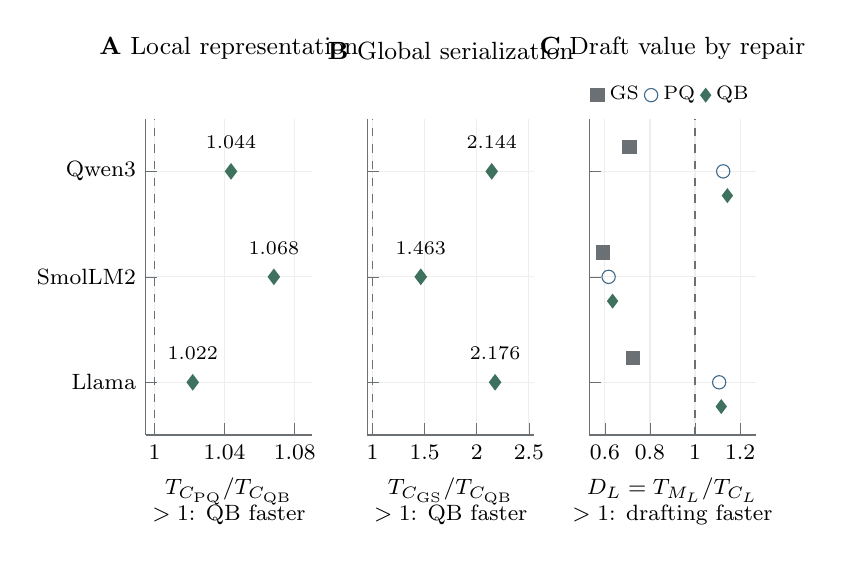
\begin{tikzpicture}
\begin{groupplot}[group style={group size=3 by 1,horizontal sep=.70cm},
width=.305\textwidth,height=5.6cm,ymin=.5,ymax=3.5,ytick={1,2,3},
tick label style={font=\footnotesize},title style={font=\small,yshift=12pt},label style={font=\footnotesize,align=center},
axis lines*=left,axis line style={aux,line width=.45pt},tick style={aux},grid=major,grid style={gray!13}]
\nextgroupplot[title={\textbf{A} Local representation},xlabel={$T_{C_{\PQ}}/T_{C_{\QB}}$\\$>1$: QB faster},xmin=.995,xmax=1.09,xtick={1,1.04,1.08},yticklabels={Llama,SmolLM2,Qwen3}]
\addplot[aux,dashed] coordinates {(1,.5)(1,3.5)};
\addplot[only marks,mark=diamond*,mark size=2.7pt,qualified] coordinates {(1.043676000000,3)};
\node[font=\scriptsize,anchor=south] at (axis cs:1.043676000000,3.12){1.044};
\addplot[only marks,mark=diamond*,mark size=2.7pt,qualified] coordinates {(1.068111000000,2)};
\node[font=\scriptsize,anchor=south] at (axis cs:1.068111000000,2.12){1.068};
\addplot[only marks,mark=diamond*,mark size=2.7pt,qualified] coordinates {(1.021848000000,1)};
\node[font=\scriptsize,anchor=south] at (axis cs:1.021848000000,1.12){1.022};
\nextgroupplot[title={\textbf{B} Global serialization},xlabel={$T_{C_{\GS}}/T_{C_{\QB}}$\\$>1$: QB faster},xmin=.95,xmax=2.55,xtick={1,1.5,2,2.5},yticklabels={,,}]
\addplot[aux,dashed] coordinates {(1,.5)(1,3.5)};
\addplot[only marks,mark=diamond*,mark size=2.7pt,qualified] coordinates {(2.143525000000,3)};
\node[font=\scriptsize,anchor=south] at (axis cs:2.143525000000,3.12){2.144};
\addplot[only marks,mark=diamond*,mark size=2.7pt,qualified] coordinates {(1.462530000000,2)};
\node[font=\scriptsize,anchor=south] at (axis cs:1.462530000000,2.12){1.463};
\addplot[only marks,mark=diamond*,mark size=2.7pt,qualified] coordinates {(2.175941000000,1)};
\node[font=\scriptsize,anchor=south] at (axis cs:2.175941000000,1.12){2.176};
\nextgroupplot[title={\textbf{C} Draft value by repair},xlabel={$D_L=T_{M_L}/T_{C_L}$\\$>1$: drafting faster},xmin=.53,xmax=1.27,xtick={.6,.8,1,1.2},yticklabels={,,},legend style={at={(.5,1.01)},anchor=south,draw=none,font=\scriptsize,fill=none},legend columns=3]
\addplot[aux,dashed,forget plot] coordinates {(1,.5)(1,3.5)};
\addplot[only marks,mark=square*,mark size=2.4pt,aux] coordinates {(0.709722260013,3.23) (0.592109590630,2.23) (0.724338602453,1.23)};
\addlegendentry{GS}
\addplot[only marks,mark=o,mark size=2.4pt,target] coordinates {(1.125118952936,3.00) (0.616360145288,2.00) (1.107396133613,1.00)};
\addlegendentry{PQ}
\addplot[only marks,mark=diamond*,mark size=2.4pt,qualified] coordinates {(1.143749000000,2.77) (0.633948000000,1.77) (1.116620000000,0.77)};
\addlegendentry{QB}
\end{groupplot}
\end{tikzpicture}
}
\caption{Matched repair and drafting choices in the original seven-arm campaign, separate from E2. A/B: speculative PQ and GS costs relative to QB. C: draft value under each repair organization, $D_L=T_{M_L}/T_{C_L}$; values above one favor drafting. Qwen3 and Llama cross parity under both local repairs, while SmolLM2 remains below it. GS/PQ values in C are reconstructed by Equation~\ref{eq:draft} from the common-panel ratios. All points are descriptive estimates; exact source ratios and every regression are retained in \sref{supp:cost}.}
\label{fig:cost}
\end{figure*}

\subsection{Seven-arm implementation comparison}
The 12-task panel comprises MBPP 123, 140, 255, 401, 413, 418 and GSM8K 111, 120, 1308, 141, 322, 443. Two adjacent sessions and four repetitions per arm/family give 2,016 formal requests and 96 qualified endpoints per arm/family. Table~\ref{tab:allcost} gives all 21 ratios. Figure~\ref{fig:taskcost} retains the task-level local-repair and draft comparisons.
\begin{table}[t]\centering\small
\caption{All 21 qualified implementation comparisons at reported six-decimal precision. Regressions count tasks on which the denominator is slower.}
\label{tab:allcost}
\begin{tabular}{@{}llrr@{}}\toprule
Family&Comparison&Ratio&Regressions\\\midrule
Qwen3 & $M_{\PQ}/M_{\QB}$ & 1.026676 & 2/12 \\
Qwen3 & $C_{\PQ}/C_{\QB}$ & 1.043676 & 0/12 \\
Qwen3 & $M_{\GS}/M_{\QB}$ & 1.330106 & 0/12 \\
Qwen3 & $C_{\GS}/C_{\QB}$ & 2.143525 & 0/12 \\
Qwen3 & $M_{\QB}/C_{\QB}$ & 1.143749 & 1/12 \\
Qwen3 & $R/M_{\QB}$ & 1.334051 & 0/12 \\
Qwen3 & $R/C_{\QB}$ & 1.525820 & 0/12 \\
SmolLM2 & $M_{\PQ}/M_{\QB}$ & 1.038478 & 0/12 \\
SmolLM2 & $C_{\PQ}/C_{\QB}$ & 1.068111 & 0/12 \\
SmolLM2 & $M_{\GS}/M_{\QB}$ & 1.366008 & 0/12 \\
SmolLM2 & $C_{\GS}/C_{\QB}$ & 1.462530 & 0/12 \\
SmolLM2 & $M_{\QB}/C_{\QB}$ & 0.633948 & 12/12 \\
SmolLM2 & $R/M_{\QB}$ & 1.369890 & 0/12 \\
SmolLM2 & $R/C_{\QB}$ & 0.868439 & 10/12 \\
Llama & $M_{\PQ}/M_{\QB}$ & 1.013407 & 1/12 \\
Llama & $C_{\PQ}/C_{\QB}$ & 1.021848 & 2/12 \\
Llama & $M_{\GS}/M_{\QB}$ & 1.411508 & 0/12 \\
Llama & $C_{\GS}/C_{\QB}$ & 2.175941 & 0/12 \\
Llama & $M_{\QB}/C_{\QB}$ & 1.116620 & 1/12 \\
Llama & $R/M_{\QB}$ & 1.426161 & 0/12 \\
Llama & $R/C_{\QB}$ & 1.592480 & 0/12 \\
\bottomrule\end{tabular}
\end{table}
\begin{figure*}[t]\centering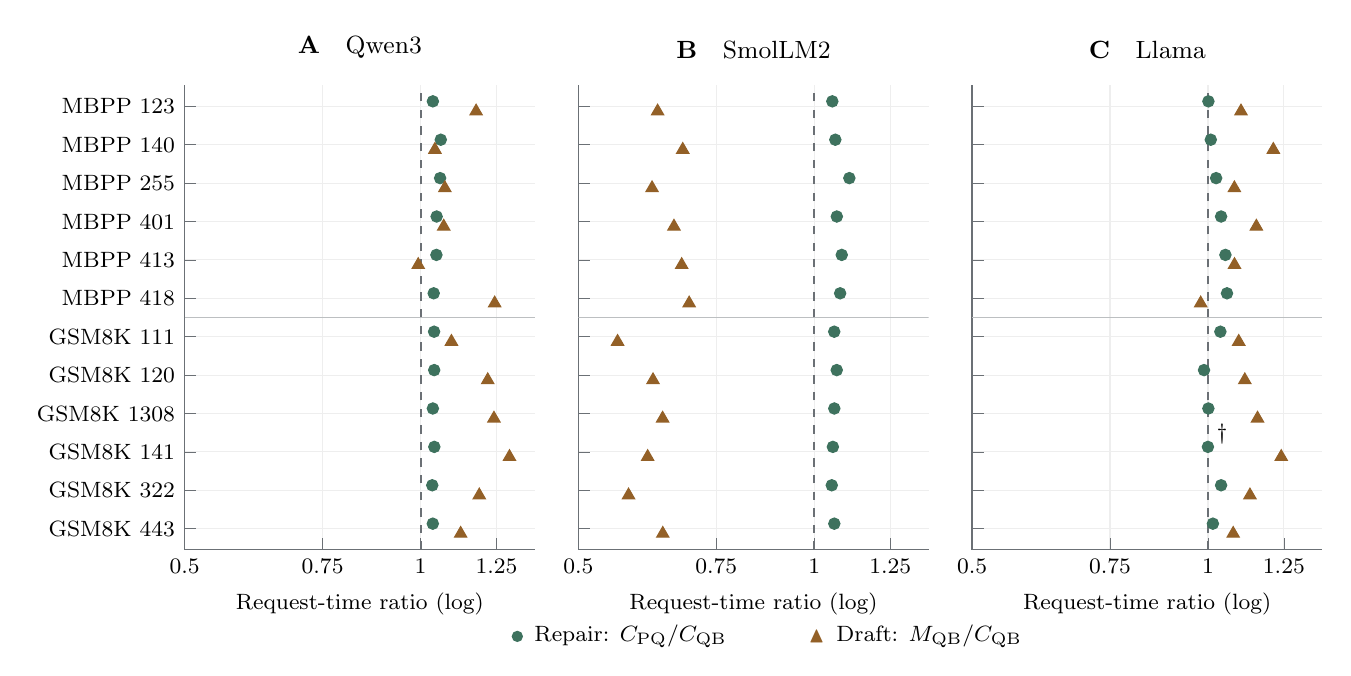
\begin{tikzpicture}[font=\footnotesize]
\pgfplotsset{tc/.style={scale only axis,width=4.45cm,height=5.9cm,
 xmin=.5,xmax=1.4,xtick={.5,.75,1,1.25},xticklabels={0.5,0.75,1,1.25},
 ymin=.45,ymax=12.55,ytick={12,11,10,9,8,7,6,5,4,3,2,1},
 tick label style={font=\footnotesize},title style={font=\small},
 xlabel={Request-time ratio (log)},xlabel style={font=\footnotesize},
 axis lines*=left,axis line style={aux,line width=.45pt},tick style={aux},grid=major,grid style={gray!13}}}
\begin{axis}[tc,xmode=log,log basis x=10,name=task0,title={\textbf{A}\quad Qwen3},yticklabels={{MBPP 123},{MBPP 140},{MBPP 255},{MBPP 401},{MBPP 413},{MBPP 418},{GSM8K 111},{GSM8K 120},{GSM8K 1308},{GSM8K 141},{GSM8K 322},{GSM8K 443}}]
\draw[aux!45,line width=.5pt] (axis cs:.5,6.5)--(axis cs:1.4,6.5);
\draw[aux,dashed,line width=.7pt] (axis cs:1,.45)--(axis cs:1,12.55);
\addplot[only marks,mark=*,mark size=2.05pt,qualified] coordinates {
(1.036885338768,12.13) % MBPP 123
(1.061278554900,11.13) % MBPP 140
(1.059180111967,10.13) % MBPP 255
(1.048438982047,9.13) % MBPP 401
(1.047751381369,8.13) % MBPP 413
(1.039442169125,7.13) % MBPP 418
(1.040676604660,6.13) % GSM8K 111
(1.040972953480,5.13) % GSM8K 120
(1.036854847813,4.13) % GSM8K 1308
(1.041304047650,3.13) % GSM8K 141
(1.035034462783,2.13) % GSM8K 322
(1.036689677369,1.13) % GSM8K 443
};
\addplot[only marks,mark=triangle*,mark size=2.55pt,draft] coordinates {
(1.177367374837,11.87) % MBPP 123
(1.043153552033,10.87) % MBPP 140
(1.074075758083,9.87) % MBPP 255
(1.070535881226,8.87) % MBPP 401
(0.993164444227,7.87) % MBPP 413
(1.243362773843,6.87) % MBPP 418
(1.095005490294,5.87) % GSM8K 111
(1.218256613173,4.87) % GSM8K 120
(1.240706906343,3.87) % GSM8K 1308
(1.298631817724,2.87) % GSM8K 141
(1.188324324823,1.87) % GSM8K 322
(1.125144610899,0.87) % GSM8K 443
};
\end{axis}
\begin{axis}[tc,xmode=log,log basis x=10,name=task1,title={\textbf{B}\quad SmolLM2},yticklabels={},at={(task0.east)},anchor=west,xshift=.55cm]
\draw[aux!45,line width=.5pt] (axis cs:.5,6.5)--(axis cs:1.4,6.5);
\draw[aux,dashed,line width=.7pt] (axis cs:1,.45)--(axis cs:1,12.55);
\addplot[only marks,mark=*,mark size=2.05pt,qualified] coordinates {
(1.054566083575,12.13) % MBPP 123
(1.063918529902,11.13) % MBPP 140
(1.108677458865,10.13) % MBPP 255
(1.068625097207,9.13) % MBPP 401
(1.084196407182,8.13) % MBPP 413
(1.079139647477,7.13) % MBPP 418
(1.060507704161,6.13) % GSM8K 111
(1.068385763399,5.13) % GSM8K 120
(1.060715564836,4.13) % GSM8K 1308
(1.056283852216,3.13) % GSM8K 141
(1.052871745769,2.13) % GSM8K 322
(1.060719024115,1.13) % GSM8K 443
};
\addplot[only marks,mark=triangle*,mark size=2.55pt,draft] coordinates {
(0.631103662893,11.87) % MBPP 123
(0.679553416367,10.87) % MBPP 140
(0.620910388381,9.87) % MBPP 255
(0.662221673125,8.87) % MBPP 401
(0.677409023433,7.87) % MBPP 413
(0.692464307030,6.87) % MBPP 418
(0.561083608097,5.87) % GSM8K 111
(0.622707419118,4.87) % GSM8K 120
(0.640490501227,3.87) % GSM8K 1308
(0.612980380488,2.87) % GSM8K 141
(0.579466032829,1.87) % GSM8K 322
(0.640824088900,0.87) % GSM8K 443
};
\end{axis}
\begin{axis}[tc,xmode=log,log basis x=10,name=task2,title={\textbf{C}\quad Llama},yticklabels={},at={(task1.east)},anchor=west,xshift=.55cm]
\draw[aux!45,line width=.5pt] (axis cs:.5,6.5)--(axis cs:1.4,6.5);
\draw[aux,dashed,line width=.7pt] (axis cs:1,.45)--(axis cs:1,12.55);
\addplot[only marks,mark=*,mark size=2.05pt,qualified] coordinates {
(1.001370147605,12.13) % MBPP 123
(1.008376337115,11.13) % MBPP 140
(1.024421134201,10.13) % MBPP 255
(1.039410861167,9.13) % MBPP 401
(1.052726772817,8.13) % MBPP 413
(1.057636679886,7.13) % MBPP 418
(1.037236647116,6.13) % GSM8K 111
(0.988542445882,5.13) % GSM8K 120
(1.001253575813,4.13) % GSM8K 1308
(0.999919059593,3.13) % GSM8K 141
(1.039432299111,2.13) % GSM8K 322
(1.014664677619,1.13) % GSM8K 443
};
\addplot[only marks,mark=triangle*,mark size=2.55pt,draft] coordinates {
(1.102019468994,11.87) % MBPP 123
(1.211831282673,10.87) % MBPP 140
(1.080833620771,9.87) % MBPP 255
(1.152939217798,8.87) % MBPP 401
(1.081181827097,7.87) % MBPP 413
(0.978890103612,6.87) % MBPP 418
(1.094724760208,5.87) % GSM8K 111
(1.114421752151,4.87) % GSM8K 120
(1.156852932560,3.87) % GSM8K 1308
(1.240381150408,2.87) % GSM8K 141
(1.131389453725,1.87) % GSM8K 322
(1.077053710346,0.87) % GSM8K 443
};
\node[anchor=south west,inner sep=0pt,xshift=3pt,yshift=1pt,font=\footnotesize] at (axis cs:0.999919059593,3.13) {$\dagger$};
\end{axis}
\coordinate (legend) at ($(task1.south)+(0,-1.10cm)$);
\fill[qualified] ($(legend)+(-3cm,0)$) circle[radius=2.05pt];
\node[anchor=west,inner sep=0pt,xshift=6pt] at ($(legend)+(-3cm,0)$) {Repair: $C_{\PQ}/C_{\QB}$};
\node[draft,inner sep=0pt] at ($(legend)+(.8cm,0)$) {$\blacktriangle$};
\node[anchor=west,inner sep=0pt,xshift=7pt] at ($(legend)+(.8cm,0)$) {Draft: $M_{\QB}/C_{\QB}$};
\end{tikzpicture}

\caption{Original repair campaign: task-level local-repair benefit $C_{\PQ}/C_{\QB}$ (circles) and draft increment $M_{\QB}/C_{\QB}$ (triangles). Session medians are combined geometrically. The dagger marks Llama GSM8K141, whose local-repair ratio is 0.999919. These are not E2 observations.}
\label{fig:taskcost}\end{figure*}

Qwen3 target-only local-repair regressions are GSM8K141 and 322. Llama regresses on MBPP418 for target-only and GSM8K120,141 for speculative local repair. SmolLM2 favors QB on all tasks in both local comparisons. Every GS/QB task favors QB. For the draft increment, Qwen3 regresses on MBPP413, Llama on MBPP418, and SmolLM2 on all 12 tasks. SmolLM2's ordinary-to-candidate comparison regresses on 10/12.

The original session-specific ratios are retained below. Target-only Qwen3 and Llama reverse direction; speculative comparisons favor QB in both adjacent sessions. E2 tests these small effects with a different, independently scheduled design and is reported separately.
\begin{table}[t]\centering\small
\caption{Original two-adjacent-session PQ/QB ratios.}\label{tab:oldsessions}
\begin{tabular}{llrr}\toprule
Family & Path & Session 0 & Session 1\\\midrule
Qwen3&M&0.971380&1.085118\\
Qwen3&C&1.041728&1.045626\\
SmolLM2&M&1.040019&1.036939\\
SmolLM2&C&1.066179&1.070046\\
Llama&M&0.994477&1.032698\\
Llama&C&1.016460&1.027264\\
\bottomrule\end{tabular}\end{table}
All original task-level and session values are retained in \texttt{anc/plot\_values.json}. The paired-ratio identities used for draft value assume the same complete panel and weights. They do not estimate attention, projection, feed-forward or synchronization shares of request time.

\begin{table}[t]\centering\small
\caption{Retrospective repair--draft contrasts reconstructed from Table~\ref{tab:allcost}. $D_L>1$ favors drafting; $\Gamma$ compares draft value under QB and GS. These are common-panel ratios, not operator-time fractions.}\label{tab:repairinteraction}
\setlength{\tabcolsep}{3pt}
\begin{tabular}{@{}lrrrr@{}}\toprule
Family & $D_{\GS}$ & $D_{\PQ}$ & $D_{\QB}$ & $\Gamma$\\\midrule
Qwen3 & 0.710 & 1.125 & 1.144 & 1.612\\
SmolLM2 & 0.592 & 0.616 & 0.634 & 1.071\\
Llama & 0.724 & 1.107 & 1.117 & 1.542\\
\bottomrule\end{tabular}
\end{table}


Table~\ref{tab:repairinteraction} makes the repair--draft comparison explicit using the existing common-panel estimates. The source values are reported to six decimal places. Propagating their rounding bounds leaves the displayed three-decimal contrasts and all draft-parity classifications unchanged. These numerical rounding bounds are separate from sampling uncertainty; the retrospective contrast adds neither requests nor a new confidence interval.

\subsection{Original-response audit of logical work}
\label{supp:sevenarmwork}
The retrospective audit reopens the original response records for all 2,016 formal requests and excludes 42 warmups. Matching family, input, session and repetition gives 288 matched seven-arm audit groups. Each group contributes one GS/PQ/QB triple for target-only execution and one for speculative execution: 576 triples and 1,728 within-path pairwise comparisons. The exported logical-work counters and acceptance/caller-width histograms agree in every comparison (Table~\ref{tab:sevenarmwork}). Complete native token-ID arrays, recorded EOG flags, length, terminal ID, stop reason, cache count and truncation flag also agree in all 1,728 non-reference-to-$R$ endpoint comparisons. Each original record's normalized IDs and workload are checked against its native response fields.

\begin{table*}[t]
\centering
\small
\begin{tabular}{lrrrr}
\toprule
Family & Matched groups & $M$ work triples & $C$ work triples & Endpoints vs. $R$ \\
\midrule
Qwen3 & 96 & 96/96 & 96/96 & 576/576 \\
SmolLM2 & 96 & 96/96 & 96/96 & 576/576 \\
Llama & 96 & 96/96 & 96/96 & 576/576 \\
\midrule
Total & 288 & 288/288 & 288/288 & 1728/1728 \\
\bottomrule
\end{tabular}
\caption{Retrospective audit of all 2,016 formal original seven-arm requests, excluding 42 warmups. Each audit group matches family, task, session and repeat across arm-specific workers; each work triple compares GS, PQ and QB within the target-only ($M$) or speculative ($C$) path. All three pairings per triple agree in the recorded logical-work counters and acceptance/width histograms (1,728 pairings total). Endpoint checks compare the complete native token IDs and recorded EOG flags, stop reason and terminal metadata with the paired $R$ request. Physical graph calls, widths and reuse are reported separately; aggregate counter equality does not establish bitwise state or per-cycle trace equality. This adds no sessions and changes no original timings or weights.}
\label{tab:sevenarmwork}
\end{table*}


The original execution has 42 family/session/arm workers, each with 48 formal requests; the second session reverses the arm order. The 288 audit groups are reconstructed by task and repetition across these workers, not collected as adjacent randomized seven-arm time blocks. Matching their recorded work does not remove between-worker temporal drift.

The counter definitions distinguish caller work from physical execution. Both GS/local contrasts change physical graph calls, graph reuse and target prefill widths in all 288 pairs per path; speculative execution also changes continuation physical-width histograms. The draft's physical counters remain equal. PQ/QB agree in every exported workload field. These are aggregate counts and histograms, not complete per-cycle trace or bitwise state comparisons. They establish matched recorded work without assigning the request-time difference to projection, attention, feed-forward computation or instrumentation.

The source manifest pins all archive parts. This audit retrieves and checks parts 001, 007 and 009 by their committed Git-blob and SHA256 identities, then verifies each selected original member against the archived index. It does not recompute the whole nine-part ZIP hash. The fixed P0 companion source at \texttt{a97f9792} includes a compressed field projection with complete endpoint arrays, original record hashes, the frozen plan, counter definitions and the original index. The present publication bundle retains the resulting table; those larger audit inputs are accessed through the pinned companion source. The reconstruction script recomputes all pairings and conservation identities from that projection. Its original-record and split-archive modes additionally reopen the archived bytes and reproduce the projection exactly. This adds no sessions and leaves all original timings and statistical weights unchanged.

Freeze versions and executable identities are distinct. The prospective v02 correction retained the 96 completed Qwen3 session-0 $R/M_{\QB}$ records under their initial freeze; the remaining 1,920 records carry v02. Actual worker commands use the metadata-capacity-corrected executable only for SmolLM2 and Llama PQ arms (384 formal requests), while the other 1,632 use the original executable. The correction enlarges PQ metadata reservation; all 21 numerical DLLs and the counter/observer sources retain identical hashes. GS/QB therefore share an executable, while the PQ comparison includes its recorded metadata-capacity correction. Exact routes and source differences remain in the audit receipt.

\section{RTX replication and numerical replay}
\label{supp:cuda}
\subsection{E2 design and complete estimates}
The replication retains the 12-task implementation panel and the original reference, models, sampler, timer and runtime routes. Each session has 54 fresh workers: short PQ/QB blocks and serial-reference blocks, with one registered warmup per worker. Across six sessions this gives 864 PQ/QB requests, 432 references and 324 warmups. Each task/session has two matching serial-reference endpoints. All required endpoints and observation checks pass; no latency is trimmed.

The fixed runtime routes use the original executable for every Qwen3 arm and all R/QB arms. SmolLM2 and Llama PQ arms use the recorded metadata4 correction; both builds retain identical hashes for all 21 numerical DLLs. The source/build manifests identify each route. The launcher clears inherited GGML/CUDA environment overrides, but neither that configuration nor GGML topology reuse establishes actual CUDA Graph replay. Per-request capture, replay and fallback counts are absent from the recovered E2 report records.

\texttt{E2\_REQUEST\_LATENCIES.csv} retains all 1,620 rows, including the 324 labelled warmups, with its original Git-blob identity. \texttt{generate\_e2\_absolute\_cost.py} checks the source and reconstructs Table~\ref{tab:e2absolute}. The per-arm geometric means use the same 12-task and six-session weights as Equation~\ref{eq:ratio}, so their quotients reproduce the paired ratios. The table's \texttt{latency\_ms} is the resident request interval; raw start/end nanosecond fields remain in the full request archive.

All consecutive session gaps exceed one hour; first-to-last start is 24.450801 hours. The original interpreter bytes were restored after a pre-start identity mismatch before the final session. The original freeze checks then passed without exception and the untouched scientific slots ran. The earlier stopped record remains part of the history.

Table~\ref{tab:e2full} gives the complete six-session estimates. The intervals use the original random seed 20261014, 10,000 bootstrap draws of six session log means, and linearly interpolated 2.5/97.5 percentiles. They quantify fixed-panel, single-host variation, not a date-level population or multiple-comparison guarantee. Table~\ref{tab:e2tasks} gives all 72 task aggregates; 9 regress. Full session contrasts and observed session times are in \texttt{anc/rtx104/}.
\begin{table*}[t]\centering\small
\caption{All completed E2 comparisons. Ratios favor QB above one; regressions count six-session task point estimates below one.}\label{tab:e2full}
\begin{tabular}{llrrrrl}\toprule
Family&Path&Ratio&Lower 95\%&Upper 95\%&Regressions&Practical threshold 1.02\\\midrule
Qwen3&M&1.020563&1.013023&1.026553&2/12&Point above; interval overlaps\\
Qwen3&C&1.031614&1.025393&1.037926&1/12&Interval above\\
SmolLM2&M&1.027767&1.021010&1.035017&2/12&Interval above\\
SmolLM2&C&1.065803&1.063387&1.068399&0/12&Interval above\\
Llama&M&1.015593&1.009627&1.021622&3/12&Point below; interval overlaps\\
Llama&C&1.029114&1.020126&1.039149&1/12&Interval above\\
\bottomrule\end{tabular}\end{table*}
\begin{table*}[t]\centering\small
\caption{E2 task-level PQ/QB ratios, geometrically averaged over six sessions. Values below one are italicized; these are descriptive task contrasts, not significance tests.}\label{tab:e2tasks}
\begin{tabular}{lrrrrrr}\toprule
&\multicolumn{2}{c}{Qwen3}&\multicolumn{2}{c}{SmolLM2}&\multicolumn{2}{c}{Llama}\\
\cmidrule(lr){2-3}\cmidrule(lr){4-5}\cmidrule(l){6-7}
Task & M & C & M & C & M & C\\\midrule
GSM8K 111&1.015305&1.028626&1.031259&1.064372&1.027335&1.029118\\
GSM8K 120&1.007356&1.073052&1.050246&1.073224&1.021427&1.026504\\
GSM8K 1308&1.018527&1.030064&1.057675&1.070511&1.020762&1.041848\\
GSM8K 141&\textit{0.992667}&1.035252&1.021013&1.051986&1.012332&1.028335\\
GSM8K 322&1.001169&1.033028&1.028420&1.059544&1.026791&\textit{0.993618}\\
GSM8K 443&1.003752&1.021251&1.033367&1.067165&1.024666&1.019558\\
MBPP 123&1.056908&1.037495&1.044148&1.058628&\textit{0.992752}&1.023365\\
MBPP 140&\textit{0.981806}&1.052058&1.041709&1.063535&\textit{0.978786}&1.048076\\
MBPP 255&1.079294&1.032638&\textit{0.972948}&1.090371&1.021555&1.054405\\
MBPP 401&1.001954&1.024979&1.044272&1.048708&1.026712&1.009394\\
MBPP 413&1.089971&\textit{0.967860}&\textit{0.978119}&1.089698&\textit{0.986121}&1.035206\\
MBPP 418&1.004440&1.046335&1.033875&1.052829&1.050112&1.041465\\
\bottomrule\end{tabular}\end{table*}

Recorded acceptance, rollback and logical-workload counters agree in all 216 speculative task/session pairs. This comparison is limited to the recorded counters and histograms, rather than complete control-trace identity. Model callers and physical micrographs remain distinct from hardware launches.

\subsection{Sensitivity to interval method and session omission}
The registered percentile bootstrap remains the primary analysis. Table~\ref{tab:e2sensitivity} adds a post-review $t$ interval,
\[
\exp\!\left(\bar z\pm t_{0.975,5}\frac{s_z}{\sqrt6}\right),
\qquad t_{0.975,5}=2.570581835636314,
\]
where $z_s$ is the session mean log contrast and $s_z$ its sample standard deviation. This analysis assumes independent, approximately normal session log means; it does not add inputs, dates or hosts. Six further point estimates omit one session each.

All speculative $t$ intervals remain above parity. Qwen3 and SmolLM2 also remain above the practical ratio threshold 1.02; Llama crosses it. Its omit-one estimates all exceed 1.02. Thus the direction of the Llama effect is stable across these checks, while its practical-threshold conclusion depends on the interval method. The source CSV is unchanged; \texttt{scripts/generate\_e2\_sensitivity.py} reconstructs the new table and the complete omit-one estimates.
\begin{table*}[t]\centering\small
\caption{E2 session sensitivity on the fixed 12-input panel. Ratios are PQ/QB; $M$ is target-only and $C$ is speculative. The registered bootstrap remains primary. Secondary $t_5$ intervals assume independent, approximately normal session log means. The final column gives the range of six leave-one-session-out point estimates.}\label{tab:e2sensitivity}
\begin{tabular}{@{}llrrrr@{}}\toprule
Family & Path & Estimate & Primary bootstrap 95\% CI & Secondary $t_5$ 95\% CI & Omit-one range\\\midrule
Qwen3 & $M$ & 1.020563 & [1.013023, 1.026553] & [1.011013, 1.030204] & [1.018397, 1.023944]\\
Qwen3 & $C$ & 1.031614 & [1.025393, 1.037926] & [1.022587, 1.040720] & [1.029113, 1.034273]\\
SmolLM2 & $M$ & 1.027767 & [1.021010, 1.035017] & [1.017648, 1.037987] & [1.024785, 1.030395]\\
SmolLM2 & $C$ & 1.065803 & [1.063387, 1.068399] & [1.062196, 1.069422] & [1.064882, 1.066443]\\
Llama & $M$ & 1.015593 & [1.009627, 1.021622] & [1.006830, 1.024433] & [1.013457, 1.018003]\\
Llama & $C$ & 1.029114 & [1.020126, 1.039149] & [1.015387, 1.043026] & [1.024960, 1.032333]\\
\bottomrule\end{tabular}
\end{table*}


\subsection{Retrospective draft-on/off analysis}
\label{supp:e2draft}
For each family, session and input, the reanalysis pairs exactly one non-warmup record from each of $M_{\mathrm{PQ}},M_{\mathrm{QB}},C_{\mathrm{PQ}},C_{\mathrm{QB}}$. There are 216 complete four-arm cells (864 measured requests). The 324 registered warmups and 432 serial-reference measurements are excluded from these contrasts after their source accounting and recorded endpoint metadata are checked. Each session averages twelve task log ratios; the reported estimate averages the six session means. Pointwise exploratory $t_5$ intervals use the six session log means with no multiplicity adjustment. These contrasts were selected retrospectively and do not replace the original primary E2 comparisons or their registered bootstrap analysis. These intervals retain the fixed-input, single-host scope of E2 and do not add a native execution or repeat full token-array qualification. The saved block order is M before C in four of six Qwen3 sessions, three of six SmolLM2 sessions and four of six Llama sessions; the remaining sessions reverse that order. Thus the M/C contrasts use separately scheduled within-session blocks, not newly randomized adjacent per-input M/C measurements, and do not isolate block-order or temporal-drift effects.

The local-layout interaction is $\Gamma=D_{\mathrm{QB}}/D_{\mathrm{PQ}}=(C_{\mathrm{PQ}}/C_{\mathrm{QB}})/(M_{\mathrm{PQ}}/M_{\mathrm{QB}})$. Its estimates are 1.010828, 1.037008 and 1.013313 for Qwen3, SmolLM2 and Llama. The exploratory intervals span parity for Qwen3 and Llama; SmolLM2's interval is [1.027962,1.046134]. Thus an improvement in draft value from QB does not itself imply profitable drafting, as the SmolLM2 result demonstrates.

The six-session QB task aggregates favor drafting for 10/12 Qwen3 inputs, 11/12 Llama inputs and 0/12 SmolLM2 inputs. These task contrasts remain descriptive. The original P0 reconstruction and source-line pairings remain at the pinned companion commit. The included \texttt{analyze\_final\_revision.py} independently reconstructs the complete quartets, draft ratios and exploratory intervals from the unchanged E2 request CSV.

\begin{table}[t]\centering\small
\caption{Retrospective E2 draft values on the fixed 12-input panel: $D_L=T_{M_L}/T_{C_L}>1$ favors drafting. QB intervals are exploratory pointwise 95\% $t_5$ intervals over six session log means. E2 has no GS arm.}\label{tab:e2draft}
\begin{tabular}{@{}lrrr@{}}\toprule
Family & $D_{\mathrm{PQ}}$ & $D_{\mathrm{QB}}$ & QB interval\\\midrule
Qwen3 & 1.072 & 1.084 & [1.059, 1.109]\\
SmolLM2 & 0.576 & 0.597 & [0.582, 0.612]\\
Llama & 1.091 & 1.105 & [1.097, 1.113]\\
\bottomrule\end{tabular}
\end{table}

\begin{table*}[t]\centering\small
\caption{Exploratory E2 draft and layout--draft contrasts. Pointwise 95\% $t_5$ intervals use six session mean log ratios and assume independent, approximately normal session means; they are not multiplicity-adjusted. $\Gamma=D_{\mathrm{QB}}/D_{\mathrm{PQ}}$ measures the change in draft value between the two local layouts, not GS/local repair interaction.}\label{tab:e2draftposthocdetail}
\begin{tabular}{llrrcc}\toprule
Family & Contrast & Estimate & Pointwise 95\% interval & Sessions $>1$ & Sessions $<1$\\\midrule
Qwen3 & $D_{\mathrm{PQ}}$ & 1.072058 & [1.058882, 1.085397] & 6/6 & 0/6\\
Qwen3 & $D_{\mathrm{QB}}$ & 1.083666 & [1.059328, 1.108563] & 6/6 & 0/6\\
Qwen3 & $\Gamma$ & 1.010828 & [0.996111, 1.025762] & 4/6 & 2/6\\
SmolLM2 & $D_{\mathrm{PQ}}$ & 0.575629 & [0.563961, 0.587538] & 0/6 & 6/6\\
SmolLM2 & $D_{\mathrm{QB}}$ & 0.596931 & [0.582288, 0.611943] & 0/6 & 6/6\\
SmolLM2 & $\Gamma$ & 1.037008 & [1.027962, 1.046134] & 6/6 & 0/6\\
Llama & $D_{\mathrm{PQ}}$ & 1.090530 & [1.069862, 1.111598] & 6/6 & 0/6\\
Llama & $D_{\mathrm{QB}}$ & 1.105048 & [1.096790, 1.113369] & 6/6 & 0/6\\
Llama & $\Gamma$ & 1.013313 & [0.994814, 1.032156] & 5/6 & 1/6\\
\bottomrule\end{tabular}
\end{table*}


\subsection{E1 coverage and controls}
The independently frozen diagnostic retains all 21 numerical DLLs and changes only the two admitted capture/replay source files. Its 72 contexts use target layers $0/\lfloor L/2\rfloor/(L-1)$, both phases and $q=1$--4. One exposed text, GSM8K443, is selected by longest inherited prompt with lexical tie-breaking for each tokenizer. It has 105/126/123 prompt IDs for Qwen3/SmolLM2/Llama. Each context has a fresh worker with a counts warmup, heavy capture and counts control; each observed MQ/PQ/QB graph is replayed twice. All 72 contexts are observed and admitted; all requests and 432 operator starts complete.

The physical key extent is 256 in every capture. The per-query visible mask counts are 1 through $q$ in prefill, 106 through $105+q$ for Qwen3 continuation, 127 through $126+q$ for SmolLM2, and 124 through $123+q$ for Llama. Minimum-key selectors refer to tensor extent, not unmasked context; this is not a query-width by visible-length factorial. All exact coordinates are in \texttt{E1\_CONTEXTS.csv}.

PQ/QB bitwise equality is 72/72 at each stage. MQ/PQ and MQ/QB equality is 18/72, exclusively the $q=1$ controls. Table~\ref{tab:e1errors} retains the largest measured differences. These compare operator arrays, not next-token logits.
\begin{table}[t]\centering\small
\caption{E1 maximum MQ-to-repair differences; both repairs give the same values. PQ/QB has zero error and ULP distance at all stages.}\label{tab:e1errors}
\begin{tabular}{lrr}\toprule
Stage&Max. finite absolute&Max. finite ULP\\\midrule
QK&0.078582763671875&2,017,357,824\\
Softmax&0.0009172558784484863&96,633\\
AV&0.010433197021484375&1,953,885,696\\\bottomrule
\end{tabular}\end{table}

Large ULP distances near zero or across signs are retained rather than converted into a tolerance-based pass. Input identity is checked before and after replay against frozen hashes. Native worker module receipts are retained; the inherited standalone replay binds executable and DLL paths but does not add a separate loaded-module inventory. Kernel symbols, reduction trees and continuous residency remain unidentified.

\subsection{Restoration and interpretation}
The host downloaded and restored the authenticated E2, E1 and control archives into a fresh directory, verifying 10,179, 9,696 and 47 members. A separate interpreter reconstructed 11 analysis outputs byte-for-byte. This is same-host restoration, not an external replication. This manuscript's own checker reconstructs the six ratios and bootstrap intervals from the submitted session table, verifies the copied context/time-table identities and checks the report summaries; it does not replay the original tensor archives.

\section{Vulkan partition and retained-state experiments}
\label{supp:b570}
\subsection{Inputs and partition controls}
A uses UB512/capacity one and a whole-prompt submission; B retains that context and externally submits $128+\mathrm{remainder}$; C uses UB128 with internal partitioning. Only the final absolute prompt position requests logits. Three repeats per input/arm, one capture-off and two capture-on, give 63 requests. All B/C initial full FP32 logits, source-defined sequence-KV payloads and complete endpoints agree.
\begin{table}[t]\centering\small
\setlength{\tabcolsep}{3.3pt}
\caption{Seven original partition inputs. All B/C full endpoints and initial FP32/KV payloads agree. The first difference is A/B, zero-based.}
\begin{tabular}{@{}lrrl@{}}\toprule
Input&Prompt IDs&First difference&A/B initial state\\\midrule
GSM1248&161&47&Different\\
GSM831&133&81&Different\\
GSM1011&190&---&Different\\
GSM1249&163&---&Different\\
Prefix 1248/127&127&---&Equal\\
Prefix 1248/128&128&---&Equal\\
Prefix 1248/129&129&57&Different\\\bottomrule
\end{tabular}
\end{table}
Initial state comprises 64 F16 K/V tensors over 32 layers and recorded logical positions. Full KV payloads are retained at prefill completion; later cuts contain full logits but only KV hashes. The synthetic prefix129 difference at 57 was not added retrospectively as a capture cut.

The final follow-up contains 21 fourth-arm observations, 38 partition-sweep observations, 18 native captures, 16 shams and 40 crosses: 133 whole requests, with a zero-forward load probe separately counted. All 19 schedules are listed in Table~\ref{tab:allpart}. Driver-body hashes were authenticated only after the fourth-arm and sweep stages, which remain diagnostic rather than fully compliant confirmation. Authentication preceded the operator and restoration stages.
\begin{table}[t]\centering\small
\caption{All frozen exposed partition schedules. The final column is first output difference from A; no numerical monotonicity is inferred.}
\label{tab:allpart}
\begin{tabular}{@{}lllr@{}}\toprule
Input&Caller widths&Endpoint class&First diff.\\\midrule
1248&64+64+33&A&---\\
1248&96+65&A&---\\
1248&128+33&B/C&47\\
1248&160+1&A&---\\
831&64+64+5&A&---\\
831&96+37&A&---\\
831&128+5&B/C&81\\
831&132+1&Third class&40\\
1011&64+64+62&All&---\\
1011&96+94&All&---\\
1011&128+62&All&---\\
1011&160+30&All&---\\
1249&64+64+35&All&---\\
1249&96+67&All&---\\
1249&128+35&All&---\\
1249&160+3&All&---\\
Prefix 129&64+65&A&---\\
Prefix 129&96+33&A&---\\
Prefix 129&128+1&B/C&57\\\bottomrule
\end{tabular}
\end{table}
\begin{figure}[t]\centering\resizebox{\columnwidth}{!}{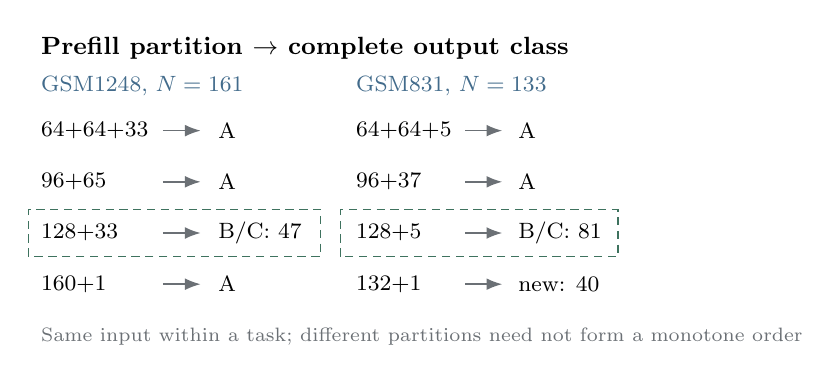
\begin{tikzpicture}[x=1cm,y=1cm,font=\footnotesize]
\node[anchor=west,font=\bfseries\small] at (0,3.35) {Prefill partition $\to$ complete output class};
\node[anchor=west,text=target] at (0,2.86) {GSM1248, $N=161$};
\node[anchor=west,text=target] at (4.0,2.86) {GSM831, $N=133$};
\foreach \y/\lab/\out in {2.3/{64+64+33}/A,1.65/{96+65}/A,1.0/{128+33}/{B/C: 47},.35/{160+1}/A}{
 \node[anchor=west] at (0,\y) {\lab};\draw[flow] (1.67,\y)--(2.15,\y);\node[anchor=west] at (2.25,\y) {\out};}
\foreach \y/\lab/\out in {2.3/{64+64+5}/A,1.65/{96+37}/A,1.0/{128+5}/{B/C: 81},.35/{132+1}/{new: 40}}{
 \node[anchor=west] at (4.0,\y) {\lab};\draw[flow] (5.51,\y)--(5.98,\y);\node[anchor=west] at (6.06,\y) {\out};}
\draw[qualified,densely dashed] (-.04,.70) rectangle (3.67,1.30);
\draw[qualified,densely dashed] (3.93,.70) rectangle (7.45,1.30);
\node[anchor=west,text=aux,font=\scriptsize] at (0,-.32) {Same input within a task; different partitions need not form a monotone order};
\end{tikzpicture}
}
\caption{Selected partition classes from the complete schedule table. A is whole prefill; B/C is the 128-split class. Numbers are first output differences from A. The map does not imply a universal 128-token threshold.}\label{fig:partition}
\end{figure}

\subsection{Projection and boundary reconstruction}
Native comparisons align actual embedding inputs, logical positions and the intended pre-attention RMS producer. Table~\ref{tab:projection} reports the layer-0 projection differences. Listing sibling projections in an audit sequence does not identify a unique first-cause kernel.
\begin{table}[t]\centering\small
\caption{Native layer-0 A/B projection differences. Values are maximum absolute differences for the stated tensors, not model-logit perturbation bounds.}
\label{tab:projection}
\begin{tabular}{@{}lrr@{}}\toprule
Projection&1248&831\\\midrule
Q&0&0.0207662582\\
K&0.0527343750&0.0703125000\\
V&0.0023193359&0.0021639541\\\bottomrule
\end{tabular}
\end{table}
Forty standalone calls compare RMS, scale/MUL and Q/K/V projections on two full/split operand geometries, with two repeats. Thirty-two pass native same-arm correspondence; eight scale/MUL calls fail because the captured input aliases a buffer already changed by an in-place consumer. Those failures remain excluded. RMS and the first task's Q controls agree bitwise, while admitted differing projection replays reproduce geometry sensitivity.

The common receiver restores sequence KV and positions, applies the native sampler to a complete 128,256-element initial FP32 vector, and reconstructs the empty generated prefix and pending token. Dynamic output buffers are rebuilt; opaque graph-cache pointers are not cloned. Sixteen own-path shams cover four inputs, both donor states and two repeats. Forty crosses then use three repeats per cell on the two affected tasks and two on the stable controls.
\begin{figure}[t]\centering\resizebox{\columnwidth}{!}{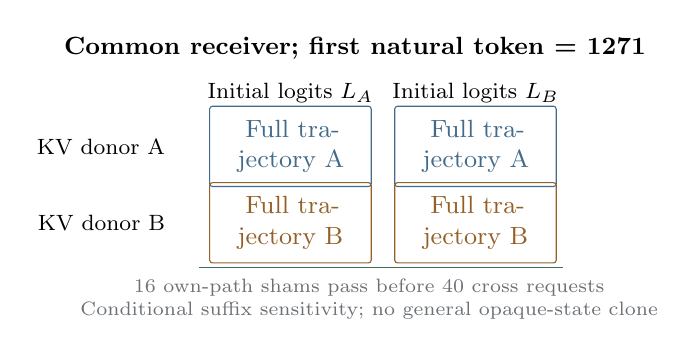
\begin{tikzpicture}[x=1cm,y=1cm,font=\footnotesize]
\node[anchor=west,font=\bfseries\small] at (0,3.35) {Common receiver; first natural token = 1271};
\node at (3.0,2.78) {Initial logits $L_A$};\node at (5.35,2.78) {Initial logits $L_B$};
\node[anchor=east] at (1.53,2.1) {KV donor A};\node[anchor=east] at (1.53,1.13) {KV donor B};
\foreach \x in {3.0,5.35}{
 \node[box,draw=target,text=target,text width=1.7cm,minimum height=.64cm] at (\x,2.1) {Full trajectory A};
 \node[box,draw=draft,text=draft,text width=1.7cm,minimum height=.64cm] at (\x,1.13) {Full trajectory B};}
\draw[qualified,line width=.6pt] (1.84,.56)--(6.46,.56);
\node[align=center,text=aux,font=\scriptsize] at (4.0,.16) {16 own-path shams pass before 40 cross requests\\Conditional suffix sensitivity; no general opaque-state clone};
\end{tikzpicture}
}
\caption{Admitted boundary0 cross for the affected tasks. All initial logits select 1271. The subsequent suffix follows the KV source under the same reconstructed receiver; stable controls retain their endpoint.}\label{fig:state}
\end{figure}

\subsection{Separate physical-work and cost boundary}
An earlier speculative actor executes a logical seed-plus-proposal verification as two occupied width-one target micrographs at $k=1$. The work-witness study retains 563 successful cycles and separate draft counts; one API-observer request failed a logging threshold and was not repeated. Its partial output is not a GPU timeline.

The original stock-relative cost campaign failed reference qualification. A later post-hoc full-output audit supports a different production-path pairing on 24 tasks and 240 repetitions: $R_{\rm prod}/C=0.719264$ and $M_{\rm match}/C=0.727927$, with every task regressing. Those negative same-output economics do not repair the original stock gate. They are not remeasured by the causal studies, and no completed component-time model is admitted.

\section{State components and decision frontiers}
\label{supp:composition}\label{supp:subsets}
\subsection{Selectors and complete endpoint matrix}
A denotes the historical whole-prefill state and B the partitioned state. Each intervention preserves recipient initial logits, natural pending-token consumption and the common receiver. Thirty-two EMPTY/ALL controls pass before the 160 subset requests. Table~\ref{tab:subsetmatrix} retains all 80 task/selector/direction coordinates; both process repeats agree. When donor and recipient natural endpoints coincide, a match is D rather than attributed to a distinguishable donor.
\begin{table*}[t]
\centering\small
\caption{All 80 distinct subset/direction coordinates. Both process repeats agree in every cell. Within each task the columns are A$\to$B and B$\to$A. B, C and D denote endpoint classes, not task-answer quality.}
\label{tab:subsetmatrix}
\begin{tabular}{@{}l*{8}{c}@{}}\toprule
 & \multicolumn{2}{c}{/1248} & \multicolumn{2}{c}{/831} & \multicolumn{2}{c}{/1011} & \multicolumn{2}{c}{/1249}\\
\cmidrule(lr){2-3}\cmidrule(lr){4-5}\cmidrule(lr){6-7}\cmidrule(l){8-9}
Selector & A$\to$B & B$\to$A & A$\to$B & B$\to$A & A$\to$B & B$\to$A & A$\to$B & B$\to$A\\\midrule
$K_0$       & B&D&C&C&C&C&D&D\\
$V_0$       & B&B&B&C&C&D&D&D\\
$K_0+V_0$   & B&D&B&C&C&D&D&D\\
All K       & D&B&C&C&C&C&D&D\\
All V       & D&B&C&C&C&C&D&D\\
Early KV    & D&D&B&C&C&D&D&D\\
Middle KV   & D&D&B&D&D&C&D&D\\
Late KV     & C&B&D&C&C&C&D&D\\
Prefix KV   & D&B&B&D&C&C&D&D\\
Tail KV     & D&B&B&D&C&C&D&D\\\bottomrule
\end{tabular}
\end{table*}
All 76 D requests change actual bytes. K-only or V-only layer0 selects $1/64$ of K/V value storage, excluding metadata. Early, middle and late groups contain 8, 16 and 8 layers. Prefix is $[0,128)$; tail is its complement, with five positions for /831. K is token-major and non-flash V feature-major, so each selector uses the actual storage strides. The source records separately retain selected bytes, changed bytes and numerical distances.

\subsection{Magnitude and common-prefix selection}
Table~\ref{tab:statenorm} reports differences computed from stored F16 values using the actual A-state norm. No increasing one-threshold rule perfectly separates these four endpoint labels: a smaller overall perturbation can accompany divergence while a larger one does not. This is a finite counterexample to a magnitude-only explanation, not an alternative predictor.
\begin{table}[t]\centering\small
\caption{Full-KV differences, B relative to A, computed from stored F16 values. Endpoint labels refer to natural A/B continuations on four exposed inputs.}
\label{tab:statenorm}
\begin{tabular}{@{}lrrl@{}}\toprule
Task & Relative $L_2$ & Max. absolute & A/B endpoint\\\midrule
/1248 &0.006488689&0.255859375&Different\\
/1249 &0.006748138&0.246093750&Same\\
/1011 &0.006887112&0.265625000&Same\\
/831  &0.010452955&1.332580566&Different\\\bottomrule
\end{tabular}
\end{table}
For each task, recipient and panel, the frontier $t^*$ is the first output at which the four natural trajectories cease to agree. Their consumed prefix is identical at that point. L0 and POSITION have separate frontiers; /831 recipient A reaches them at 40 and 81 respectively. Later vectors cannot fill an earlier missing comparison.

Archived captures support 44 of 112 planned repeat-level contrasts, with 22 agreeing pairs. The 68 incomplete comparisons contain 272 missing panel entries or 240 distinct arm/repeat/position vectors, because some arms are shared. A vector hash or top-two scores do not replace full logits. Output zero uses the frozen initial logits and needs no additional forward. Table~\ref{tab:frontier} retains every available frontier contrast.
\begin{table*}[t]\centering\small
\caption{All available frontier contrasts. L0 components are K/V; POSITION components are prefix/tail. Both historical repeats agree. Values are rounded to six decimals. Token pairs are fixed within each panel; direction-dependent coordinates must be canonicalized before comparing signs.}
\label{tab:frontier}
\begin{tabular}{@{}lllr rrrr@{}}\toprule
Task&Direction&Panel&$t^*$&$\Delta_1$&$\Delta_2$&$I$&EMPTY margin\\\midrule
1248&B$\to$A&L0&47& .059744& .088148&-.135864&.066515\\
1248&A$\to$B&L0&47& .025909& .033445&-.019032&.010706\\
1248&B$\to$A&POSITION&47& .078003& .095778&-.096560&.066515\\
1248&A$\to$B&POSITION&47&-.018557&-.000782& .096560&.010706\\
831&B$\to$A&POSITION&81&-.095177&-.062551& .238718&.013084\\
831&A$\to$B&L0&81& .118263& .172575&-.049446&.067905\\
831&A$\to$B&POSITION&81& .143541& .176167&-.238718&.067905\\\bottomrule
\end{tabular}
\end{table*}
For /1248 B$\to$A L0 at 47, the additive joint prediction is $0.08137702941894531$, the actual joint is $-0.05448722839355469$ and $I_{KV}=-0.1358642578125$. Full-vocabulary argmax is 220/220/832/220. At output46, the same fixed-pair residual is $-0.13482666015625$, but the actual top two are 11/220 with margin $8.017614364624023$; the frontier pair 220/832 is not that position's top two. Cross-position comparison is descriptive.

At output1 of /1011, EMPTY margins are $0.561777115/0.549312592$, maximum observed $\epsilon_\infty=0.207827211$, and every arm satisfies $m>2\epsilon_\infty$ and selects 11886. The mixed trajectories later diverge at 10, whose adjacent full vectors are missing. For /1249 the corresponding margins are $0.959617615/0.936807632$, maximum $\epsilon_\infty=0.194167793$, and every observed arm selects 1505. This sufficient top-1 condition applies only at the measured position.

\subsection{Direction symmetry and independent conditions}
For complete states $(A_P,A_T)$ and $(B_P,B_T)$, reversing donor and recipient permutes the POSITION quartet from AA, BA, AB, BB to BB, AB, BA, AA. When the actual state, prefix and receiver agree under this mapping,
\begin{equation}
\boldsymbol I=\boldsymbol z_{\rm ALL}-\boldsymbol z_P-\boldsymbol z_T+\boldsymbol z_{\rm EMPTY}
\end{equation}
is invariant. The scalar $I(u)-I(r)$ changes sign when $(r,u)$ is reversed. The audit checks actual state, FP32 vectors, prefixes, sampling conditions and F64 bytes in all 12 available direction pairs. For /1248 at47 both directions give $-0.09655952453613281$ in pair order $(220,832)$, despite opposite original signs.

Of the 44 oriented repeat rows, 24 are POSITION and 20 L0. Accounting for direction symmetry and two repeats gives six POSITION and ten oriented L0 conditions, still only four underlying inputs. L0 has different surrounding recipient states and is not collapsed by the POSITION identity.

\subsection{Acquisition failure and data scope}
A new acquisition attempted one request with a registry key missing recipient identity. The planned EMPTY B$\to$A imported B rather than A, completing 127 decodes before failing the input check. It is neither a qualified EMPTY nor an ALL sample; 167 slots were unstarted. The later CPU revision repairs request assembly without new native data. The 54 unique FP32 vectors and 16 residual vectors support the historical 44 contrasts; no missing frontier or independent-machine GPU replication is supplied by that revision.

\section{Natural-execution port and backend audit}
\label{supp:pilot}
\subsection{Design and complete exploratory endpoints}
The natural pilot keeps the original ordinary UB128/capacity-one reference R. R\_SHADOW tests the rebuilt actor without replacing R. Candidate prefill uses reference128 or bulk512 organization, MQ attention and capacity4. Six speculative arms use continuation MQ/PQ/QB, target UB4, $k=1$ and the same draft; two arms are draft-free. Every request starts from its prompt without imported state.

The planned 80 requests are eight original R, four shadow counts, four shadow diagnostics, 32 candidate counts and 32 candidate diagnostics. It stops with 49 attempts, 48 complete, one interrupted and 31 unstarted. Table~\ref{tab:pilot} preserves all 14 endpoint counterexamples. The reference and shadow outputs agree, but candidate observer pairs are incomplete. The q1 branch bypasses the multi-query transformation, so draft-free QB-labelled agreement does not qualify lifted QB.
\begin{table}[t]\centering\small
\caption{Complete candidate counts endpoints observed before stopping. Values are first differing output indices from original R; ``='' denotes an equal complete cap128 endpoint. Candidate observer pairs are incomplete. The execution-contract limitation prevents qualification of this panel.}
\label{tab:pilot}
\begin{tabular}{@{}lrrrrr@{}}\toprule
Arm&/1248&/831&/1011&/1249&Matches\\\midrule
$M_{B,\QB}$&47&81&=&=&2/4\\
$M_{R,\QB}$&=&=&=&=&4/4\\
$C_{B,\MQ}$&47&40&10&=&1/4\\
$C_{B,\PQ}$&47&81&=&=&2/4\\
$C_{B,\QB}$&47&40&10&=&1/4\\
$C_{R,\MQ}$&=&40&10&=&2/4\\
$C_{R,\PQ}$&=&=&=&=&4/4\\
$C_{R,\QB}$&=&81&10&=&2/4\\\bottomrule
\end{tabular}
\end{table}
The frozen monitoring declaration requires 100ms request-period VRAM sampling. The original R instead supplies four checkpoints, with maximum gaps 2874--3033ms. The mismatch is detected while the 49th request is active; only its owned worker is terminated. No sampled threshold violation was observed, but the original declaration remains unmet. P2/P3 are not executed and qualified speedup remains null. The 8,110 caller events, full times and raw accounting are retained in the ancillary record.

The available candidate diagnostics contain histograms but no ordered, phase-bound multirow VERIFY witness, leaving actual multirow placement unresolved. Descriptive request times include the new actor's observation, lifecycle and phase-management costs as well as attention.

\subsection{Independent representation audit}
The follow-up uses the same frozen CPU numerical libraries across 144 development and 288 locked held-out synthetic fixtures. It covers $q\in\{1,2\}$, key extents 127/128/129/255/256/257, head pairs $(8,8),(8,1),(32,8)$, $d=128$, and compact or legally offset model-permuted Q. Three nonempty masks and two fixed data patterns give 72 geometries and 432 fixtures; MQ/PQ/QB require 1,296 CPU graph evaluations. Held-out here refers to synthetic test conditions, not new model prompts.

An independent integer oracle checks addresses, contiguous-group GQA, mask columns and output recovery. Four injected faults are detected. A separate FP64 scalar oracle uses stored inputs. Structured one-hot and single-valid-key tests have exact expectations. No strict assertion, crash or nonfinite failure occurs. General differences remain descriptive: maximum absolute error is zero at QK on the dyadic inputs, $5.3608031\!\times\!10^{-9}$ at softmax, and $5.5132505\!\times\!10^{-5}$ at AV/final output. No post-hoc tolerance defines a general numerical pass. F16-representable dyadic data do not establish generic F32 reduction invariance.

The complete historical endpoints satisfy $M_{B,\QB}=C_{B,\PQ}$, $M_{R,\QB}=C_{R,\PQ}$ and $C_{B,\MQ}=C_{B,\QB}$ on all four windows. On /1011, $C_{R,\MQ}$ and $C_{R,\QB}$ both first differ at10 but have different full endpoints. These relations do not establish common operands, KV or acceptance traces.

\subsection{Version-bound support semantics}
Seven core backend/header hashes match the archived build manifest and the numerical DLLs are unchanged. The frozen \texttt{ggml\_backend\_vk\_device\_supports\_op} rejects the reviewed QK and AV shapes because their fourth source extents are $(1,2)$. The complete source identity and line location are in \texttt{anc/portability111.json}. Unbound shader bodies are excluded from arithmetic attribution.

The descriptor checker rejects the unequal fourth extents and leaves other cases unresolved because equality is only one necessary admission condition. This CPU/source analysis identifies the backend change required before a same-backend numerical comparison. Actual routing and fallback remain unknown, and the stopped pilot retains its failed qualification.

\section{Mapping, representation and observer controls}
\label{supp:followupmapping}
The post-replication mapping studies retain distinct references, input sets, runtimes and timers~\cite{mappingrecords,b570compactrecords}. Their results are not additional samples of the original E2 experiment. The full scientific heads and paths are in \texttt{anc/source\_manifest.json} and the follow-up evidence index.

\subsection{Input lifetime and software controls}
The original RTX allocation allowed later AV and ordinary-output nodes to overwrite storage holding K/V. Address and byte witnesses, re-upload interventions and return to the original allocation localized this failure. Independent persistent input storage restored repeated input and output bytes. This repair establishes valid repeated execution; it supplies no accelerator result.

Balanced PQ/QB/QH comparisons use identical QB\_A/QB\_B controls. The core $q=2,4$ panel yields QB\_A/QH=0.900826, with 19 of 24 geometries supporting lower QB cost under the declared descriptive screen and five unresolved. A/A pilot envelope reduction to a median 2.762\% does not establish 2\% precision for each geometry. A selector predicts all 12 held-out synthetic mean directions but costs 1.010298 times fixed QB once the measured lookup is charged; its estimate is an offline phase sum, not an integrated request.

CUDA Graph ON is established through capture, instantiation and replay in instrumented hosts. Clean hosts share the graph/runtime identity without loading the observer. The ON/OFF intervention reduces QB\_A completed-graph cost to 0.615--0.849 of OFF. Profiling traces identify path changes, but kernel durations do not supply a union of busy time or a request critical path.

\subsection{Fixed-logical-input padding and cost windows}
Logical-length-preserving padding keeps original mask columns and appends finite zero K/V with fully masked keys. L1023/S1024 fails all four reference qualifications despite reaching three kernels at the first observed execution. L1023/S1025 qualifies all four, retains eight kernels and costs 1.014783/1.014974 times the two native controls. L1024/S1025 and L1024/S1026 also fail the exact reference. All failed paths stop at the first mismatch; no clean steady-state benefit is reported for them. Source-to-DLL correspondence for the internal RTX divergence remains unknown.

The complete RTX Q transaction begins with common permuted host Q and includes copy/transpose, Q upload/completion, graph replay/synchronization and full ordinary readback. For $q=2,4$, compact-QH/QB\_A is 1.002216/1.001598 and compact-QH/QB\_B is 1.008295/1.004167. K/V/mask are resident and targets preallocated; the interval excludes natural Q generation and continuing KV updates.

The B570 equal-head panel instead uses Hq/Hkv=8/8, $d=128$, key1023/1024/1025 and $q=1,2,4$. Its narrow admission repair enables the existing batch-broadcast shader without K/V REPEAT. Three fixed input sets and three process sessions, balanced over both identical QB controls and QH, give a resident-graph difference of $-1.028\,\mu$s [$-2.177,+0.067$]. The separately measured complete representation transaction gives $-1.518\,\mu$s [$-4.168,+0.916$], ratio 0.992244 [0.979908,1.004691]. These are descriptive adjusted intervals from three process clusters on one device/date; all practical-effect screens remain unresolved. The 43,740 transactions are technical repetitions, not independent workloads. The two windows cannot be subtracted to isolate transfer cost.

\subsection{Request relevance and observer integrity}
The first B570 Qwen3 request bridge is a separate q1/key256/GQA32:8 observation. It does not exercise the equal-head near1024 micrograph. Serial per-operation logging adds about 12\% median decode overhead and fails its 10\% observer screen. Concurrent logging initially omits the terminal interval and includes inactive-node labels; terminal timestamps and the executor's active-node predicate repair those faults.

The final same-DLL clean/profile/clean medians are 27.6675/29.6058/27.6794 ms, so the observer still adds about 7\%. Each final context table counts 16 output projections and 5,004 QK, softmax, AV and CONT operations each. The third-context GPU subtotal is 3.490070 s over prefill and continuation. Pure QK/softmax/AV contributes 2.8005\%, or at most 2.8026\% when the mixed group is included; the core excludes projections, RoPE and KV updates. Quantized matvec/fused groups contribute 92.5152\% and contain both attention projections and FFN. These diagnostic fractions are not clean request shares or a bandwidth diagnosis.

\section{Historical finite-panel service results and prefill closeout}
\label{supp:service}
\subsection{Panel identities and qualification}
Table~\ref{tab:servicecontracts} lists the two service contracts. Each panel has four exposed inputs, $k=1$, 32/8 target GQA, F16 KV and actual two-query verification in all 36 target layers. The draft and target models are Qwen3-0.6B and Qwen3-8B Q8\_0. Model/tokenizer hashes and exact driver identities are pinned separately; the shared family names do not make these a paired GPU experiment.

\begin{table*}[t]\centering\small
\caption{Distinct service contracts. The entries describe the recorded experiments, not recommended production configurations.}
\label{tab:servicecontracts}
\begin{tabularx}{\textwidth}{@{}p{3.0cm}YY@{}}\toprule
Property & RTX service study & B570 formal request study\\\midrule
Reference and inputs & New R/PQ full-logit references, historical native endpoints; MBPP/413, GSM8K/120,322,443 & Prospective q1 reference; HumanEval/38,65,115,127 with their recorded chat formatting\\
Output window & Native EOG or cap128 & Native EOG or cap64\\
Target/draft capacity & R target UB1; speculative target UB4; draft UB1 & Target verification UB4; draft UB1; serialized q1 prefill\\
Context and host policy & Context1024, 24 host threads & Context1024, eight context thread parameters\\
Measurement & 64 requests in four timing processes; 64 explicit warmups & 64 requests in four timing processes; 16 explicit warmups\\
Qualification & Eight reference requests and 12 independent qualification requests; 1,106+1,794 vectors & 12 qualification requests; 346 saved PQ/QB full-logit pairs\\
Primary window & Fresh-context creation/reservation through prefill, generation, state/synchronization and teardown & Same declared service components; separate private driver and prefill policy\\
Excluded / separately charged & Shared model loading, post-timer comparison and raw-file I/O & Shared model loading, post-timer comparison and raw-file I/O\\\bottomrule
\end{tabularx}\end{table*}

The RTX source/driver registration precedes every model start; its independently generated R/PQ reference is sealed before qualification, and the qualification record is sealed before timing~\cite{rtxservicerecords}. R uses its matching reference; PQ and QB use the matching PQ target/draft vectors, including rejected verification rows. Their complete speculative traces also agree. This does not assert that every internal PQ value equals a serial R value. Query geometry and mask extents/strides are observed, whereas visible-key counts are derived from the registered causal positions. No operator readback is inserted into the natural CUDA graph.

The B570 AV repair first passes six synthetic key256/512 by $q=1,2,4$ coordinates with unchanged PQ stage files, then a model integration passes one exposed 16-token bridge. Its first cost pilot preserves a 5.123483-second discrepancy between identical PQ arms. The apparently favorable aggregate is not promoted into a speedup. A separately registered four-input panel uses a 64-token cap and natural EOG, and qualifies complete R/PQ/QB endpoints, 346 PQ/QB vectors and full speculative cycle traces before timing~\cite{b570gqarecords,b570servicerecords}. The old Llama Q6\_K references and their failures remain separate.

\subsection{Every input and paired block}
\begin{table*}[t]\centering\small
\caption{All input-aggregate service ratios. Four sessions contribute to each row. A/A is the ratio of two identical PQ controls. Lower QB ratios favor QB. Inputs are different between platforms.}\label{tab:serviceinputs}
\begin{tabular}{@{}llrrrr@{}}\toprule
Platform & Input & Output / stop & QB / dual-PQ & QB / R & PQ\_A / PQ\_B\\\midrule
RTX & MBPP/413 & 34/EOG & 0.988025 & 0.608126 & 0.947919\\
RTX & GSM8K/120 & 128/CAP & 1.004279 & 0.578678 & 0.956661\\
RTX & GSM8K/322 & 128/CAP & 0.963695 & 0.610027 & 0.990391\\
RTX & GSM8K/443 & 128/CAP & 1.001663 & 0.535651 & 0.964986\\
\textbf{RTX} & \textbf{Equal-weight mean} & --- & 0.989284 & 0.582325 & ---\\\midrule
B570 & HumanEval/38 & 64/CAP & 0.994638 & 2.597826 & 0.999532\\
B570 & HumanEval/65 & 53/EOG & 0.992003 & 2.652017 & 0.997703\\
B570 & HumanEval/115 & 41/EOG & 0.997281 & 2.619785 & 0.999881\\
B570 & HumanEval/127 & 64/CAP & 0.996663 & 2.609733 & 0.992463\\
\textbf{B570} & \textbf{Equal-weight mean} & --- & 0.995144 & 2.619763 & ---\\\bottomrule
\end{tabular}
\end{table*}

\begin{table*}[t]\centering\footnotesize
\caption{Every input/session block from the two service panels. Each platform has its own input set; adjacent rows do not form cross-platform pairs. Exact source blocks are included in the ancillary CSV files.}\label{tab:serviceblocks}
\begin{minipage}[t]{.485\textwidth}\centering
\textbf{RTX}\par\vspace{4pt}
\setlength{\tabcolsep}{3pt}\begin{tabular}{@{}rlrrr@{}}\toprule
$s$ & Input & QB/PQ & QB/R & A/A\\\midrule
0 & M/413 & 1.139826 & 0.860710 & 0.995684\\
0 & G/120 & 0.945850 & 0.626761 & 0.948687\\
0 & G/322 & 0.923908 & 0.620302 & 1.002893\\
0 & G/443 & 0.922590 & 0.536318 & 0.937857\\
1 & M/413 & 1.037841 & 0.605209 & 1.018199\\
1 & G/120 & 1.060687 & 0.598746 & 0.928511\\
1 & G/322 & 0.964679 & 0.643793 & 1.133151\\
1 & G/443 & 1.095851 & 0.587714 & 0.908679\\
2 & M/413 & 0.867052 & 0.507936 & 0.836860\\
2 & G/120 & 1.075364 & 0.574851 & 0.996817\\
2 & G/322 & 1.063244 & 0.656443 & 0.950265\\
2 & G/443 & 1.031135 & 0.530409 & 1.012026\\
3 & M/413 & 0.929090 & 0.516898 & 0.951652\\
3 & G/120 & 0.942870 & 0.519815 & 0.953907\\
3 & G/322 & 0.910152 & 0.528264 & 0.890920\\
3 & G/443 & 0.965632 & 0.492411 & 1.005416\\
\bottomrule\end{tabular}\end{minipage}
\hfill
\begin{minipage}[t]{.485\textwidth}\centering
\textbf{B570}\par\vspace{4pt}
\setlength{\tabcolsep}{3pt}\begin{tabular}{@{}rlrrr@{}}\toprule
$s$ & Input & QB/PQ & QB/R & A/A\\\midrule
0 & HE/38 & 0.994435 & 2.594996 & 1.000263\\
0 & HE/65 & 0.994347 & 2.670002 & 0.998378\\
0 & HE/115 & 0.997636 & 2.622364 & 0.999695\\
0 & HE/127 & 0.998560 & 2.603504 & 1.001035\\
1 & HE/38 & 0.995388 & 2.601387 & 0.997047\\
1 & HE/65 & 0.990654 & 2.645055 & 1.001826\\
1 & HE/115 & 0.997896 & 2.619781 & 1.000689\\
1 & HE/127 & 0.997328 & 2.604889 & 0.998169\\
2 & HE/38 & 0.997377 & 2.602636 & 1.001209\\
2 & HE/65 & 0.992339 & 2.647094 & 0.997665\\
2 & HE/115 & 0.996576 & 2.619385 & 0.998640\\
2 & HE/127 & 0.998198 & 2.602524 & 0.998604\\
3 & HE/38 & 0.991360 & 2.592299 & 0.999614\\
3 & HE/65 & 0.990676 & 2.645998 & 0.992961\\
3 & HE/115 & 0.997017 & 2.617613 & 1.000503\\
3 & HE/127 & 0.992578 & 2.628099 & 0.972324\\
\bottomrule\end{tabular}\end{minipage}
\end{table*}

\begin{figure*}[t]
\centering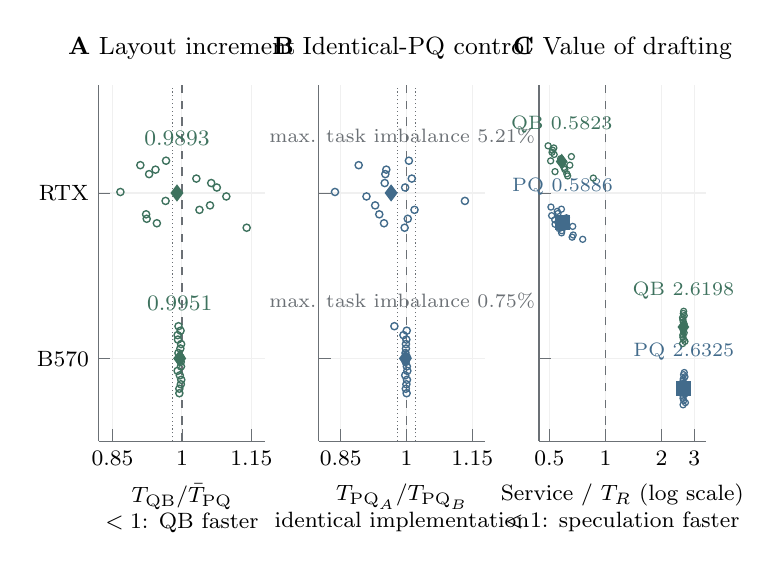
\begin{tikzpicture}
\begin{groupplot}[group style={group size=3 by 1,horizontal sep=.68cm},
width=.305\textwidth,height=6.1cm,ymin=.5,ymax=2.65,ytick={1,2},
tick label style={font=\footnotesize},title style={font=\small},label style={font=\footnotesize,align=center},
axis lines*=left,axis line style={aux,line width=.45pt},tick style={aux},
grid=major,grid style={gray!12},clip=false]
\nextgroupplot[title={\textbf{A} Layout increment},xlabel={$T_{\QB}/\bar T_{\PQ}$\\$<1$: QB faster},xmin=.82,xmax=1.18,xtick={.85,1,1.15},yticklabels={B570,RTX}]
\addplot[aux,dashed,line width=.65pt] coordinates {(1,.5)(1,2.65)};
\addplot[aux,densely dotted] coordinates {(.98,.5)(.98,2.65)};
\addplot[only marks,mark=o,mark size=1.3pt,mark options={draw=qualified,fill=white,line width=.5pt},qualified] coordinates {(1.139826244244,1.790) (0.945849532204,1.817) (0.923908031504,1.844) (0.922589990337,1.871) (1.037840796194,1.898) (1.060687483585,1.925) (0.964678996272,1.952) (1.095850644734,1.979) (0.867051748054,2.006) (1.075364022151,2.033) (1.063243809835,2.060) (1.031135431587,2.087) (0.929089961795,2.114) (0.942869964094,2.141) (0.910151770722,2.168) (0.965631764151,2.195)};
\addplot[only marks,mark=diamond*,mark size=2.8pt,qualified] coordinates {(0.989283832162,2)};
\node[font=\footnotesize,text=qualified,anchor=south] at (axis cs:0.989283832162,2.23){0.9893};
\addplot[only marks,mark=o,mark size=1.3pt,mark options={draw=qualified,fill=white,line width=.5pt},qualified] coordinates {(0.994434518096,0.790) (0.994346955730,0.817) (0.997636159223,0.844) (0.998559725528,0.871) (0.995388158443,0.898) (0.990654252807,0.925) (0.997896355971,0.952) (0.997327956447,0.979) (0.997377153779,1.006) (0.992338895142,1.033) (0.996575875826,1.060) (0.998197853655,1.087) (0.991359732503,1.114) (0.990675696924,1.141) (0.997016709214,1.168) (0.992578048127,1.195)};
\addplot[only marks,mark=diamond*,mark size=2.8pt,qualified] coordinates {(0.995143975812,1)};
\node[font=\footnotesize,text=qualified,anchor=south] at (axis cs:0.995143975812,1.23){0.9951};
\nextgroupplot[title={\textbf{B} Identical-PQ control},xlabel={$T_{\PQ_A}/T_{\PQ_B}$\\identical implementation},xmin=.80,xmax=1.18,xtick={.85,1,1.15},yticklabels={,}]
\addplot[aux,dashed,line width=.65pt] coordinates {(1,.5)(1,2.65)};
\addplot[aux,densely dotted] coordinates {(.98,.5)(.98,2.65)};
\addplot[aux,densely dotted] coordinates {(1.02,.5)(1.02,2.65)};
\addplot[only marks,mark=o,mark size=1.3pt,mark options={draw=target,fill=white,line width=.5pt},target] coordinates {(0.995683567795,1.790) (0.948687206972,1.817) (1.002893498473,1.844) (0.937857123081,1.871) (1.018199057240,1.898) (0.928511175631,1.925) (1.133151458846,1.952) (0.908678851591,1.979) (0.836859699631,2.006) (0.996816614475,2.033) (0.950265018054,2.060) (1.012025769051,2.087) (0.951652309469,2.114) (0.953906893171,2.141) (0.890919556111,2.168) (1.005416311802,2.195)};
\addplot[only marks,mark=diamond*,mark size=2.8pt,target] coordinates {(0.964859750025,2)};
\node[font=\scriptsize,text=aux,anchor=south] at (axis cs:0.99,2.24){max. task imbalance 5.21\%};
\addplot[only marks,mark=o,mark size=1.3pt,mark options={draw=target,fill=white,line width=.5pt},target] coordinates {(1.000263373246,0.790) (0.998378236952,0.817) (0.999694644835,0.844) (1.001035132081,0.871) (0.997047068817,0.898) (1.001825902924,0.925) (1.000688705872,0.952) (0.998169208021,0.979) (1.001209202542,1.006) (0.997665280704,1.033) (0.998639552710,1.060) (0.998604248688,1.087) (0.999614281800,1.114) (0.992960821525,1.141) (1.000503281379,1.168) (0.972323667784,1.195)};
\addplot[only marks,mark=diamond*,mark size=2.8pt,target] coordinates {(0.997390415137,1)};
\node[font=\scriptsize,text=aux,anchor=south] at (axis cs:0.99,1.24){max. task imbalance 0.75\%};
\nextgroupplot[title={\textbf{C} Value of drafting},xlabel={Service / $T_R$ (log scale)\\$<1$: speculation faster},xmode=log,log basis x=10,xmin=.44,xmax=3.45,xtick={.5,1,2,3},xticklabels={0.5,1,2,3},yticklabels={,}]
\addplot[aux,dashed,line width=.65pt] coordinates {(1,.5)(1,2.65)};
\addplot[only marks,mark=o,mark size=1.1pt,mark options={draw=qualified,fill=white,line width=.45pt},qualified] coordinates {(0.860709500935,2.090) (0.626760614714,2.103) (0.620301508760,2.116) (0.536318432454,2.129) (0.605208924945,2.142) (0.598746155267,2.155) (0.643792756015,2.168) (0.587714386461,2.181) (0.507935515395,2.194) (0.574851260097,2.207) (0.656442531287,2.220) (0.530408922715,2.233) (0.516897971637,2.246) (0.519814743067,2.259) (0.528263723757,2.272) (0.492411464129,2.285)};
\addplot[only marks,mark=diamond*,mark size=2.5pt,qualified] coordinates {(0.582325110976,2.190)};
\node[font=\scriptsize,text=qualified,anchor=south] at (axis cs:0.582325110976,2.300){QB 0.5823};
\addplot[only marks,mark=o,mark size=1.1pt,mark options={draw=target,fill=white,line width=.45pt},target] coordinates {(0.755123428050,1.720) (0.662643045616,1.733) (0.671388804522,1.746) (0.581318286640,1.759) (0.583142353976,1.772) (0.564488753316,1.785) (0.667364748795,1.798) (0.536308838513,1.811) (0.585819146937,1.824) (0.534564341243,1.837) (0.617396052735,1.850) (0.514393072401,1.863) (0.556348677623,1.876) (0.551311170004,1.889) (0.580412784714,1.902) (0.509937102744,1.915)};
\addplot[only marks,mark=square*,mark size=2.5pt,target] coordinates {(0.588633001010,1.820)};
\node[font=\scriptsize,text=target,anchor=south] at (axis cs:0.588633001010,1.930){PQ 0.5886};
\addplot[only marks,mark=o,mark size=1.1pt,mark options={draw=qualified,fill=white,line width=.45pt},qualified] coordinates {(2.594995842505,1.090) (2.670002306074,1.103) (2.622363844693,1.116) (2.603504205863,1.129) (2.601387062271,1.142) (2.645054922828,1.155) (2.619781081148,1.168) (2.604889445075,1.181) (2.602635519004,1.194) (2.647093847080,1.207) (2.619384718054,1.220) (2.602523908884,1.233) (2.592298609216,1.246) (2.645997993711,1.259) (2.617612598821,1.272) (2.628099334862,1.285)};
\addplot[only marks,mark=diamond*,mark size=2.5pt,qualified] coordinates {(2.619762936381,1.190)};
\node[font=\scriptsize,text=qualified,anchor=south] at (axis cs:2.619762936381,1.300){QB 2.6198};
\addplot[only marks,mark=o,mark size=1.1pt,mark options={draw=target,fill=white,line width=.45pt},target] coordinates {(2.609519073689,0.720) (2.685181757420,0.733) (2.628577383096,0.746) (2.607259374984,0.759) (2.613439832700,0.772) (2.670008143944,0.785) (2.625303785781,0.798) (2.611868471385,0.811) (2.609479783192,0.824) (2.667530074694,0.837) (2.628384633415,0.850) (2.607222505392,0.863) (2.614891975358,0.876) (2.670902296209,0.889) (2.625445064894,0.902) (2.647750813975,0.915)};
\addplot[only marks,mark=square*,mark size=2.5pt,target] coordinates {(2.632546646573,0.820)};
\node[font=\scriptsize,text=target,anchor=south] at (axis cs:2.632546646573,0.930){PQ 2.6325};
\end{groupplot}
\end{tikzpicture}

\caption{Service costs under separate platform contracts. Small outlined points show all 16 input/session blocks per contrast; large markers are equal-weight geometric means. A: QB/dual-PQ. B: identical-PQ A/A, with the largest absolute input-aggregate imbalance used by the screen. C: both speculative paths relative to target-only R. Dashed lines mark parity; dotted lines show 2\%. Vertical offsets separate observations. Ratios below one favor the numerator. The platform panels are analyzed separately.}
\label{fig:servicepanels}
\end{figure*}
The tables and Figure~\ref{fig:servicepanels} are generated from the saved block records. RTX blocks retain all four arm service times, permitting direct recomputation of each ratio. B570 aggregates are reconstructed from archived paired ratios; the original service logs and full raw logits are outside the manuscript package. \texttt{anc/check\_closure.py} verifies exact Git blob identities, weights, input/session coverage, ratios, plot coordinates and printed cells.

The primary layout estimator gives equal weight to each input and session in log space. Its A/A criterion is the largest absolute per-input geometric-mean PQ\_A/PQ\_B deviation from one, not the largest individual block deviation. The finite engineering screen also requires more than 2\% reduction and all session aggregates below one. RTX session ratios are 0.979094, 1.038635, 1.005512 and 0.936718, and the A/A criterion is 5.208\%. B570 session ratios are 0.996243, 0.995313, 0.996120 and 0.992904, with A/A criterion 0.754\%; its 0.486\% layout point reduction is below 2\%. Neither panel passes the practical layout screen.

All 16 RTX QB/R blocks are below one and all 16 B570 QB/R blocks exceed one. Aggregate ratios are 0.582325 and 2.619763 respectively. RTX dual-PQ/R is 0.588633, showing that the speculative-policy benefit is already present with PQ. The RTX estimate corresponds to a 41.8\% service-time reduction; throughput uses the inverse time ratio. These four-input panels report descriptive paired estimates and every process-session block.

Warmups are separately recorded, but their presence alone establishes neither cold-driver behavior nor warmed state for all shapes. B570 uses the old 16-token key256 request for warmup; key512 pipeline persistence across processes is uncontrolled. The RTX panel warms each input/arm. Continuous exclusive device ownership is not established in either study. All blocks and reversals are retained; no outlier deletion or significance-driven extension is used.

\subsection{Draft-policy counterfactual and completed prefill follow-up}
The B570 thread-parameter study fixes the PR134 QB references and changes draft context parameters from 8 to 1 while keeping the target at 8. All 346 vectors and endpoints/state traces remain unchanged. Four timing processes yield 64 measurements plus 16 warmups. DRAFT1/dual-baseline service is 1.003994, DRAFT1/R is 2.633056 and the A/A criterion is 0.793\%. The session ratios 0.998803, 1.007142, 1.010567 and 0.999512 do not support a practical improvement~\cite{b570policyrecords}. A temporary ggml pool object in an OpenMP build does not establish per-call creation of OS threads; the one-task GET\_ROWS/SET\_ROWS plan can clamp effective workers before the parameter takes effect.

The same reviewed commit also contains a draft-prefill submission follow-up. Its first attempt fails an observer-axis check; this failure is retained. A prospective observer-only repair checks the consumed QK tensor and all four inputs then qualify, with 346 matching logits, one draft-prefill API call and physical prefill $q=1$. A later registered closeout completes this cost comparison under its separate CPU-draft service contract~\cite{b570prefillrecords}. It records 156 requests: four calibration, 24 qualification, 64 matched warmups and 64 measurements. SUBMIT/dual-baseline is 0.999161, a 0.084\% point reduction against 0.369\% input-aggregate A/A and a 2\% practical floor. One session favors the baseline. Fewer submissions therefore do not establish lower complete service cost, and QB/thread8 remains the baseline. SUBMIT/R is 1.203678 in this later contract; it cannot be compared with PR134's 2.619763 as a controlled improvement because device placement and service policy differ. The recorded helper-process reservation was not a complete observed count; full resource-protocol compliance is not established. The valid negative cost result and that accounting limitation are both retained.

\subsection{Evidence and execution accounting}
The RTX study completes 12 native processes and 148 requests: eight references, 12 qualification, 64 measured and 64 warmups. All native exits and cleanup are recorded, with no scientific retry. The conditional 24 profiling slots remain unstarted under the registered stopping rule. Native parent lifetime is 446.746733 seconds; GPU-active time is unmeasured. The preparation staging failure is retained, and its earlier compiler lifetime was not captured.

The locally retained RTX archive contains 3,110 members and 2,900 vectors and is 2,270,281,687 bytes. The originating host reports reopening and hashing every member. The present manuscript package contains reported blocks, derived values, source identities and the original consistency inputs; it does not contain that full native archive. Local restoration, GitHub compact-record reconstruction and independent full-raw access are different evidence levels. B570's original full vectors also remain separately held.

\section{Matched deployment, input transfer and native reproduction}
\label{supp:followup}
\subsection{Frozen matched design and uncertainty}
The RTX bridge freezes at \texttt{30ad53be} before six formal process sessions. Its twelve-input panel is MBPP/123,140,255,401,413,418 and GSM8K/111,120,1308,141,322,443. Each session measures every input in four cells and three arms, giving $6\times12\times4\times3=864$ measurements; twelve warmup requests per session add 72. All 936 requests complete without formal retries, missing slots or outlier removal. Each cell occupies each order position three times per session. Each cell/session uses every three-arm permutation twice; each input/cell uses all six permutations across sessions.

The primary estimator is the exponential of the equal-input, equal-session mean of $\log[T_{\QB}/\operatorname{mean}(T_{\PQ_A},T_{\PQ_B})]$. The registered 20,000-resample bootstrap jointly resamples the six session vectors, preserving the four paired cells. Each cell uses a 98.75\% percentile interval, yielding nominal 95\% family coverage across four primary cells. Practical success additionally requires an upper ratio below 0.98, a point reduction above both 2\% and the input-aggregate A/A imbalance, and improvement in every session. With six sessions on one date, these intervals describe process-session variation on that host; date-level uncertainty is unmeasured.

The absolute arithmetic PQ/QB service means are 1.646575/1.631283 seconds for $k=1$ resident, 1.358022/1.272156 for $k=3$ resident, 1.690768/1.655382 for $k=1$ fresh and 1.371483/1.307389 for $k=3$ fresh. Ratios of these arithmetic means need not equal the primary geometric paired estimate. All per-input regressions, session signs, omit-one-session, chronological and pointwise $t$ sensitivities remain in the archived analysis. The secondary $k3/k1$ ratios of layout ratios are 0.950119 resident and 0.972137 fresh; lifecycle contrasts are 0.986740 at $k=1$ and 1.009607 at $k=3$, with pointwise intervals spanning one for both lifecycle contrasts. The interaction is exploratory.

\subsection{Preserved engineering attempts and observation cost}
A 25-request pilot precedes qualification. The first qualification attempt completes 135 requests before a Windows aggregate-file replacement failure leaves 69 slots unexecuted. A recording-only correction creates a new executable identity, and all 204 qualification requests are rerun before freezing formal timing. No formal samples are pooled across builds. A counter pilot has an unresolved approximately 2.9\% difference, so the additional counters and heavy callback/logit capture are off during formal timing. Common driver bookkeeping, phase timers and inherited backend logging remain included. Actual CUDA capture/replay/fallback activity is not fully recorded.

\subsection{Previously unexposed panel and stopped families}
The input-transfer study is separately frozen and does not share the bridge's exposed-input claim. It reaches 33 of 36 family/input cells, representing 20 of 21 distinct tasks. Independent compact reconstruction reconciles 1,018 completed and 758 unexecuted request slots; the two qualified families contribute 384 measurements and 384 warmups. No successful Llama subset is timed after its reference counterexample. Initial missing raw-offset metadata is retained; a heavy-observer correction and causal rules are fixed before held-out selection. The native-fast path fails old calibration for SmolLM2/Llama and held-out GSM8K/70 for Qwen3. Source-pinned counterexample token IDs, dispositions and all cost rows accompany the paper.

\subsection{Native evidence and access}
RTX restores 3,542 original and 3,537 metadata4 source members, rebuilds core/frontend objects, and retains the pinned numerical DLLs. A real Qwen3 layer0/q3 fixture passes original/rebuilt MQ/PQ/QB replay with two repeats; six original/rebuilt HTTP R/PQ/QB requests match the historical endpoint. The subsequent delivery kit provides the real fixture, complete request references, formal records and exact numerical-dependency acquisition; the full 38,078-file raw directory remains separately held.

B570 rebuilds all five numerical libraries and 147 shader translation units from source. A new HumanEval/115 layer0/q2/key512 capture and its first-query q1 slice pass 16 stage comparisons. The ordinary four-input R/PQ/QB panel matches 914 historical complete vectors plus outputs, stops and state; copied-directory execution passes again. A diagnostic capture/supervision correction retains identical numerical DLL hashes. All 21 model requests and two stage workers are accounted for; nine additional cumulative Job processes lack identities/lifetimes. These resource limits do not change the recorded numerical comparisons. The original 1.37 GB archive remains in source-host custody. The subsequent authenticated delivery publishes the source/stage/request subset and all four inputs' complete historical reference vectors. This reproduces PR134's two-model Vulkan contract, not PR143's later CPU-draft service policy.

\texttt{anc/followup\_20261026/} carries exact compact records, source pins, derived tables and a read-only reconstruction path. The present manuscript revision performs CPU analysis only. Native build and replay results above are the platform executions recorded in the cited campaigns.

\section{Three-date scope transfer and final producer-state tests}
\label{supp:finaltransfer}
\subsection{RTX execution and estimator}
The frozen seven-arm study reuses the complete twelve-input Qwen3 and SmolLM2 panels from the earlier natural-input transfer. It is a new runtime cohort, not a new blind input selection. Within each family, all seven arms share the executable, core, numerical DLLs, model bytes and resident-context lifecycle. GS selects physical target width one; PQ/QB preserve surrounding multirow work. Target-only and speculative requests can share a cleared target context within a fixed scope, never across scopes. Model loading and resident provisioning occur before registered warmups.

Qualification executes $2\times12\times7=168$ heavy requests plus 28 observer-off sentinels, for 196 total. Each of twelve independently loaded family-session processes then executes twelve contiguous seven-arm blocks and seven warmups: $12\times84=1,008$ measurements and $12\times7=84$ warmups. All 1,288 requests complete with no missing slots or technical/numerical retries. The original October 29 start elapsed without formal requests; the disclosed October 30/31/November 1 calendar amendment was committed and authorized before formal collection. The original calendar remains part of the history.

The seven-arm base permutation is rotated by session and source-input index. Six rotations per input across six sessions yield arm-position counts differing by at most one over the 72 blocks per family. Input order is frozen by hash, and family-first order alternates by date. The first sessions of adjacent date slots satisfy the registered 20-hour gates. All measured requests remain within their actual Asia/Shanghai dates.

For input $i$, session $s$ and date $d$, let $z_{dsi,L}=\log[T(M_L)/T(C_L)]$. The study first averages the twelve input log ratios, then its two session means, then its three date means. The same weights apply to $I=z_{\QB}-z_{\GS}$ and all secondary contrasts. No old campaign is pooled into these estimates.

\begin{table*}[t]\centering\small
\caption{Three-date scope--draft results. $D_L=T_{M_L}/T_{C_L}>1$ favors drafting; $\Gamma=D_{\QB}/D_{\GS}$. Inputs, sessions within date and dates receive equal log weights.}\label{tab:scopefinal}
\begin{tabular}{@{}llrrrr@{}}\toprule
Family & Date / pooled & $D_{\GS}$ & $D_{\PQ}$ & $D_{\QB}$ & $\Gamma$\\\midrule
Qwen3 & 2026-10-30 & 0.829731 & 1.099220 & 1.128913 & 1.360577\\
Qwen3 & 2026-10-31 & 0.839248 & 1.159931 & 1.220335 & 1.454082\\
Qwen3 & 2026-11-01 & 0.835003 & 1.107396 & 1.218402 & 1.459158\\
\textbf{Qwen3} & \textbf{Pooled} & 0.834652 & 1.121863 & 1.188438 & 1.423874\\\midrule
SmolLM2 & 2026-10-30 & 0.676863 & 0.751980 & 0.762481 & 1.126491\\
SmolLM2 & 2026-10-31 & 0.691716 & 0.828542 & 0.829419 & 1.199075\\
SmolLM2 & 2026-11-01 & 0.684117 & 0.838157 & 0.824490 & 1.205188\\
\textbf{SmolLM2} & \textbf{Pooled} & 0.684205 & 0.805284 & 0.804877 & 1.176367\\\bottomrule
\end{tabular}
\end{table*}

\begin{table*}[t]\centering\small
\caption{All six session means per family in the three-date study. A session averages its twelve input log contrasts. The 1,008 requests are not independent date samples.}\label{tab:scopesessions}
\begin{tabular}{@{}llrrrrr@{}}\toprule
Family & Date & Session & $D_{\GS}$ & $D_{\PQ}$ & $D_{\QB}$ & $\Gamma$\\\midrule
Qwen3 & 2026-10-30 & 0 & 0.830111 & 1.096315 & 1.130326 & 1.361658\\
Qwen3 & 2026-10-30 & 1 & 0.829352 & 1.102133 & 1.127501 & 1.359497\\
Qwen3 & 2026-10-31 & 0 & 0.866651 & 1.142133 & 1.221022 & 1.408897\\
Qwen3 & 2026-10-31 & 1 & 0.812711 & 1.178006 & 1.219649 & 1.500716\\
Qwen3 & 2026-11-01 & 0 & 0.827459 & 1.104158 & 1.221824 & 1.476599\\
Qwen3 & 2026-11-01 & 1 & 0.842617 & 1.110644 & 1.214989 & 1.441924\\
SmolLM2 & 2026-10-30 & 0 & 0.676932 & 0.758510 & 0.762756 & 1.126783\\
SmolLM2 & 2026-10-30 & 1 & 0.676795 & 0.745507 & 0.762206 & 1.126200\\
SmolLM2 & 2026-10-31 & 0 & 0.686908 & 0.830144 & 0.817371 & 1.189927\\
SmolLM2 & 2026-10-31 & 1 & 0.696557 & 0.826943 & 0.841644 & 1.208292\\
SmolLM2 & 2026-11-01 & 0 & 0.685719 & 0.840344 & 0.817952 & 1.192839\\
SmolLM2 & 2026-11-01 & 1 & 0.682519 & 0.835977 & 0.831080 & 1.217666\\
\bottomrule\end{tabular}
\end{table*}

\begin{table*}[t]\centering\small
\caption{Secondary three-date ratios and registered weak date-sensitivity intervals. QB/PQ ratios below one favor QB; $R/C$ compares a different baseline and is not the draft increment. The intervals are conditional $t_2$ sensitivity summaries, not robust population uncertainty.}\label{tab:scopesecondary}
\begin{tabular}{@{}lrrrrrl@{}}\toprule
Family & $C_{\QB}/C_{\PQ}$ & $M_{\QB}/M_{\PQ}$ & $R/C_{\GS}$ & $R/C_{\PQ}$ & $R/C_{\QB}$ & $\Gamma$ sensitivity\\\midrule
Qwen3 & 0.954407 & 1.011045 & 0.812867 & 2.022730 & 2.119357 & [1.236342, 1.639850]\\
SmolLM2 & 0.934678 & 0.934205 & 0.709091 & 1.346225 & 1.440309 & [1.028092, 1.346028]\\
\bottomrule\end{tabular}
\end{table*}


All three date means and all six session means have positive $I$. The full source analysis retains 5/72 negative Qwen3 input/session effects and 27/72 negative SmolLM2 effects; no reversal is removed. Qwen3's recorded logical work is matched across scopes. SmolLM2's is not, so its effect includes the changed speculative path. The secondary Qwen3 target-only QB/PQ ratio changes direction across dates. Its pooled ratio must not be described as an improvement in every session.

The registered 97.5\% two-sided sensitivity interval for each primary family contrast is
\[
\exp\!\left(\overline I\pm t_{0.9875,2}\frac{s_I}{\sqrt3}\right),
\qquad t_{0.9875,2}=6.205346816570706.
\]
The two-primary-family Bonferroni allocation assumes independent approximately normal date means. With three dates it is a weak sensitivity summary, not robust population uncertainty or power. The main figure shows the actual three date means and their range. Session repeats and the 1,008 measured requests are not treated as independent dates.

The original source auditor reads all 1,288 request records and associated payloads. This editorial reconstruction independently checks the twelve reported session log vectors, their date and aggregate algebra, and the exact B570 compact CSVs below. It does not rerun the RTX raw-request or full-vector auditor. \texttt{anc/final\_20261101/SOURCE\_INDEX.json} distinguishes these evidence levels.

\subsection{Bounded Llama diagnostic}
\label{supp:finaldiagnostic}
A separate 54-request stream retains the known CodeContests/valid/108 counterexample and two controls, CodeContests/valid/43 and GSM8K/test/496. A1 executes three inputs by $R/C_{\PQ}/C_{\QB}$ by observer-off/heavy, giving 18 requests. A2 executes the three inputs by P1/P4\_NATIVE by target-only C1/$C_{\PQ}/C_{\QB}$ by observer setting, giving 36. A0 reads historical evidence and executes no model request.

The known failure reproduces under both observer settings, and both controls match historical $R$. In A2, target-only C1 retains $R$ under both producer recipes on the known input, whereas speculative PQ/QB still agree with each other and depart from $R$. All observer pairs retain the outcome, and paired captured vectors match for PQ/QB. The audit records 5,916 vectors. These naturally generated recipes do not import a common state and therefore do not isolate a consumer-only intervention. No earliest internal operator is identified, no repair is established and diagnostic clocks are excluded from performance analysis.

\subsection{B570 producer--consumer matrix}
\label{supp:finalproducer}
The Qwen3-8B/0.6B Q8\_0 experiment retains both models on B570 Vulkan, eight host threads, non-flash attention and F16 KV. P1 and P4T use the same PQ target producer, UB4/output4, token IDs, positions and final-only logits flags. P1 submits one ID at a time; P4T uses width four with a fixed tail-three split into two plus one. Draft production remains the same independent serial recipe for every speculative consumer.

The full producer boundary contains sequence-KV serialization, positions and initial full FP32 logits. Each clean receiver imports the selected boundary, verifies actual post-import readback and consumes the initial logits exactly once. C1 is target-only; PQ/QB use the unchanged $k=1$ transaction. The intervention tests the total boundary-state effect, not a KV-only component effect.

The 32 historical controls include natural/resumed C1 and consumer-specific PQ/QB own-path comparisons with observer-off/heavy guards. On the eight selected inputs, each independently executed strict UB1/output1 $R$ is compared with natural P1+C1. Natural P1/P4T C1, C1 restoration and local PQ/QB continuations supply 120 further requests. All 152 primary requests execute once; 96 actual boundaries and 88 observer/own-path comparisons pass the recorded raw audit. The resulting 48 scientific cells are all evidence-qualified, while only 39 equal strict $R$.

\begin{table*}[t]\centering\small
\caption{Complete B570 producer-conditioned endpoint outcomes. Local combines PQ and QB, whose endpoints, cycles and captured vectors agree within every producer. Strict $R$ and own-producer C1 comparisons have different denominators.}\label{tab:producerfull}
\begin{tabular}{@{}lrrrrrr@{}}\toprule
Input & Prompt IDs & P1 C1=$R$ & P4T C1=$R$ & P1 local=C1 & P4T local=C1 & First P1 departure\\\midrule
GSM8K/582 & 83 & yes & yes & yes & yes & ---\\
GSM8K/4140 & 68 & yes & yes & yes & yes & ---\\
GSM8K/1184 & 118 & yes & no & no & no & 30\\
GSM8K/2279 & 68 & yes & yes & yes & yes & ---\\
MATH/prealgebra/1865 & 265 & yes & yes & no & yes & 5\\
MATH/geometry/846 & 274 & yes & yes & yes & yes & ---\\
MATH/prealgebra/1804 & 343 & yes & yes & no & yes & 25\\
MATH/geometry/465 & 302 & yes & yes & yes & yes & ---\\
\bottomrule\end{tabular}
\end{table*}


The 16 input--producer PQ/QB pairs agree in complete endpoints, cycles and all captured full-vocabulary vectors, including discarded verification rows. Both serialized KV and initial logits change on 8/8 inputs. Five inputs retain $R$ across all six cells. Prealgebra/1865 and /1804 switch local eligibility while natural C1/$R$ remains fixed; their first departures are one-based outputs 5 and 25. GSM8K/1184 instead changes its natural C1 endpoint under P4T, first at output 30; local continuations differ from their own C1 at outputs 30 and 32 under P1 and P4T.

The source pool was amended before new model forwards after static exposure and length checks could not fill the requested bands. Four original GSM8K and four original MATH-500 problems were chosen by the frozen hash rule, without output- or timing-based selection, truncation or concatenation. The retained panel is mathematical throughout; source and length are confounded. Exact input strings, selection records and static stops remain in the source archive. Natural integrated P4T speculative production was not qualified by this clean-receiver experiment, and its diagnostic resource times are not formal service estimates.

\subsection{Final evidence delivery}
RTX's immutable base through date zero and Llama diagnostics has 39 object ZIPs, 8,541 unique objects and 38,087 original-path mappings. Date-one and date-two increments add three ZIPs each, containing 425 and 427 members respectively. B570 publishes six ZIPs plus two manifest/receipt assets containing 6,826 files. Source-host authenticated downloads and readback checks are recorded for every batch; B570's frozen CPU analysis recreates eight outputs byte-for-byte from that downloaded copy. These are source-host delivery checks, distinct from independent-host native reproduction.

The publication source includes exact B570 matrix/state CSVs and an explicitly labelled projection of the RTX session log contrasts. Its CPU script reconstructs all new printed ratios and figures, with fixed-source provenance. Bulk raw vectors, execution capsules and models are accessed separately through the fixed companion records. The new evidence commits are \texttt{29511ed9} for RTX and \texttt{022babfa} for B570. No new model execution is performed by this manuscript revision.

\balance
\section{Reproduction and evidence access}
\label{supp:reproduction}
A single \texttt{main.tex} builds the article and supplement. The source package contains editable figures, original reported cost/state matrices, recovered E2 request times, saved service blocks and compact follow-up results. Standard-library analysis scripts verify source hashes, accounting, the registered E2 bootstrap, retrospective contrasts and generated tables. Original binary64 derived summaries allow one adjacent value for math-library rounding; the final reported-log reconstruction uses a $2\times10^{-13}$ numerical tolerance. Input bytes, integer counts and generated TeX are checked separately.

The final analysis consumes twelve RTX session-level log vectors transcribed from the pinned complete analysis and two exact B570 CSVs. Their manifest distinguishes transcription from exact source copying. It reconstructs date/pooled ratios and matrix counts; the 1,288-request RTX audit and all full-vector checks remain the recorded platform audits. The earlier P0 seven-arm raw-response projection and its original audit code are available at the fixed paper commit \texttt{a97f9792}; they are not duplicated in this smaller publication package. Its summary table and conclusions are preserved. This bundle can reconstruct the retrospective E2 draft contrasts directly from the included 1,620-row CSV.

\texttt{anc/runtime\_reproduction/} supplies CPU interface tests and archived implementation patches with provenance. Companion native kits add builds, real fixtures and request references~\cite{rtxnativebridge,b570nativereproduction}. RTX rebuilds the core/frontend while retaining pinned numerical DLLs; a real $q=3$ fixture and complete requests reproduce historical outputs. B570 rebuilds five numerical libraries and 147 shader translation units; a real $q=2$ fixture, its $q=1$ slice and the four-input request panel reproduce stage bytes and 914 historical full-logit vectors. These are source-host native executions, not independent-machine replications.

Authenticated delivery kits now expose source, fixtures, complete request references and exact dependency acquisition~\cite{rtxnativedelivery,b570nativedelivery}. RTX's twelve-part kit and relocation checks retain 785 indexed payload files and 704 request vectors. B570's minimal and four-input reference packages include download audits, a 175-vector capture/reference comparison and a 914-vector stored-reference consistency check. The larger final-experiment archives and their readback receipts are described in \sref{supp:finaltransfer}. Repository authentication and external model acquisition remain necessary; full native archives are not embedded in the arXiv source.

\texttt{REPRODUCTION\_ACCESS.md} and \texttt{anc/source\_manifest.json} provide immutable source locations and evidence scope. The 28 legacy groups and their scientific dispositions remain in \texttt{anc/historical\_disposition.csv} and the ancillary history. The archived AV hardware model is a same-policy parity control. Historical failures, missing vectors and unexecuted slots keep their original status. Generated TeX tables remain outside \texttt{anc/}, so article compilation does not depend on ancillary-file handling.

\end{document}
